The design \& development of the Mirrorshades platform was driven both to investigate mobile PR systems as a concept in general \& to assess their suitability when applied to a particular case study as a new modality for interacting with virtual content within the context of a cultural heritage site. For this purpose evaluation of the platform firstly addressed its reception compared to a `traditional' virtual heritage experience \& secondly studied reactions to/preferences toward different PR implementations with regards to the default view \& transition styles provided.

%=========================================================================================================

%Final video
%\url{https://www.youtube.com/watch?v=UsDRPjDwr8A}
%screenshots

%=========================================================================================================

\section{Overview}

The evaluation process was divided into two stages; the first assessed the utility of Mirrorshades as a mobile PR platform in comparison to existing VR techniques used within a virtual heritage context, while the second investigated participants' preferences \& reactions to different transition styles, in order to inform further PR implementations. A combination of qualitative \& quantitative data were collected for both stages, as the nature of the platform experience is such that purely quantitative data is not sufficient to gain an insight into the desired metrics, but is nonetheless useful to corroborate, or rebut, qualitative responses \& observations.

Participants were sourced by adverts disseminated via an internal university memo system, which sends an email to all registered staff \& students each week. The advert appeared for several consecutive weeks. Participants were invited to take part in a \textit{`virtual reality study \ldots\ investigating different ways of switching your view between your real surroundings \& a virtual environment'}. Participation was incentivised by a prize draw to win Amazon vouchers. This approach was adopted instead of sourcing participants from within the OVW group \& (computer science) department, as participants with a heightened knowledge \&/or interest in the technology underlying the platform were expected to skew results by paying conscious attention to the system \& its implementation rather than the actual experience of using the system. In total 17 participants, 10x male \& 7x female, with a mean age of 23.1 years \& a standard deviation of 4.9 years, took part in the user studies, each lasting 20-30 minutes. All studies took place at St Salvator's chapel during afternoon hours, with the chapel open to the general public.

%=========================================================================================================

\section{Stage 1 - PR for Virtual Heritage}

Previously when VR has been employed in virtual heritage scenarios, it has predominantly been implemented as CAVE experiences~\cite{Roussou2002}. Visitors to a museum or visitor centre will be offered the opportunity to step into a CAVE, possibly donning shutter glasses or similar apparatus to enable a stereoscopic 3D effect, to experience a VR reconstruction of a location, its contents \& actors. Some of these CAVE installations have featured physical control interfaces such as joystick \& 3D mouse~\cite{cabral:x3dexperience} \& haptic interfaces~\cite{Christou2006}, while others have tracked user movement, whether head only or full body  gestures (such as in figure \ref{VTTP_projection.png}). In common among these CAVE experiences is the fact that the VR content they present is experienced with a disconnect to the RW site that it pertains to, as the CAVE itself immerses users in VR visuals \& does not permit them to see any of their RW surroundings, comparable to the experience of weareing a VR HMD without see-through video functionality. Furthermore, the physical size of the CAVE limits the amount in any particular direction that a user can physically move, even if movement is encouraged due to its use as a control methodology.

With the promise of high performance VR HMDs at a consumer price point on the horizon, thanks largely to the rejuvenation in the field effected by Oculus, their use at cultural heritage sites for achieving similar experiences to previous CAVE installations is becoming more plausible \& brings with it certain benefits such as a reduction in the physical space required at the site for the installation. The OVW group's experience with presenting both experts \& interested amateurs, young \& old, with virtual heritage content via Oculus HMDs (both DK1 \& DK2, see section \ref{virtual-heritage-at-st-andrews}) has been very promising. These interactions have taken place in scenarios similar to those of existing CAVE scenarios; the user remains physically stationary \& uses a controller or gestures to move their virtual presence throughout the VR environment, whilst unable to observe their RW environment due to the nature of the HMD isolating them from RW visual stimuli.

In this first stage of the evaluation a comparison is made of this `traditional' style of interacting with VR content at a cultural heritage site wherein VR is experienced in isolation from RW, with both temporal \& spatial separation, against the `new' style afforded by the Mirrorshades platform, in which VR can be experienced in tandem with RW by allowing the user to move around their RW environment \& transition at any time into seeing the VR environment from the equivalent vantage point. Participants in this stage of the evaluation thus complete two scenarios wherein they interact with the RW St Salvator's chapel \& its corresponding VR reconstruction;

\begin{enumerate}
	\item \textbf{Traditional scenario} - Participants experience the RW \& VR chapels separately. They navigate the VR chapel from a stationary position, as VR has traditionally been employed at cultural heritage sites via CAVE installations \& by the OVW group with Oculus HMDs, using the Xbox controller to move around the VR environment observed via the DK1, with the DK1 obscuring their view of the RW chapel around them. Subsequently, they navigate the RW chapel without the DK1 or any associated equipment.
	\item \textbf{PR scenario} - Participants experience the RW \& VR chapels in tandem using the Mirrorshades platform. They wear the DK1, holding the Xbox controller in their right hand \& the smartphone in their left, with the laptop \& control box bundle in a satchel worn over one shoulder. Pressing a button on the Xbox controller triggers a transition between RW \& VR visual stimuli being displayed by the DK1.
\end{enumerate}

%=========================================================================================================

\subsection{Design of the Scenarios}

The scenarios were intended to mimic the style of exploration \& interaction that visitors to the chapel display, after observing the behaviour of such visitors on several occasions. From these observations, a common pattern of behaviour emerged: visitors enter the chapel from the North/West corner then proceed to walk Eastwards along the nave, pausing to look around after passing through the rood screen, before continuing along the nave toward the altar. They then pause in front of the alter upon reaching the end of the pews \& then walk North toward the tomb where they pause again to inspect it. Participants in this first stage of the evaluation process were instructed to imagine that they were performing a similar visit to the chapel \& to follow a similar path, pausing after the rood screen, at the end of the pews \& in front of the tomb to look around their environment(s) in more detail, however they were encouraged to stop \& look around at any times/positions that they wished \& not to feel restricted to the specific path \& locations. The intent of the scenario was to encourage a natural style of exploration despite the unusual situation of making use of bulky VR hardware, rather than to restrict them to an `on rails' experience. Participants were shown the map included as figure \ref{chapel-path} (North upwards) to help visualise the instructions.

\begin{figure}[h]
	\begin{center}
		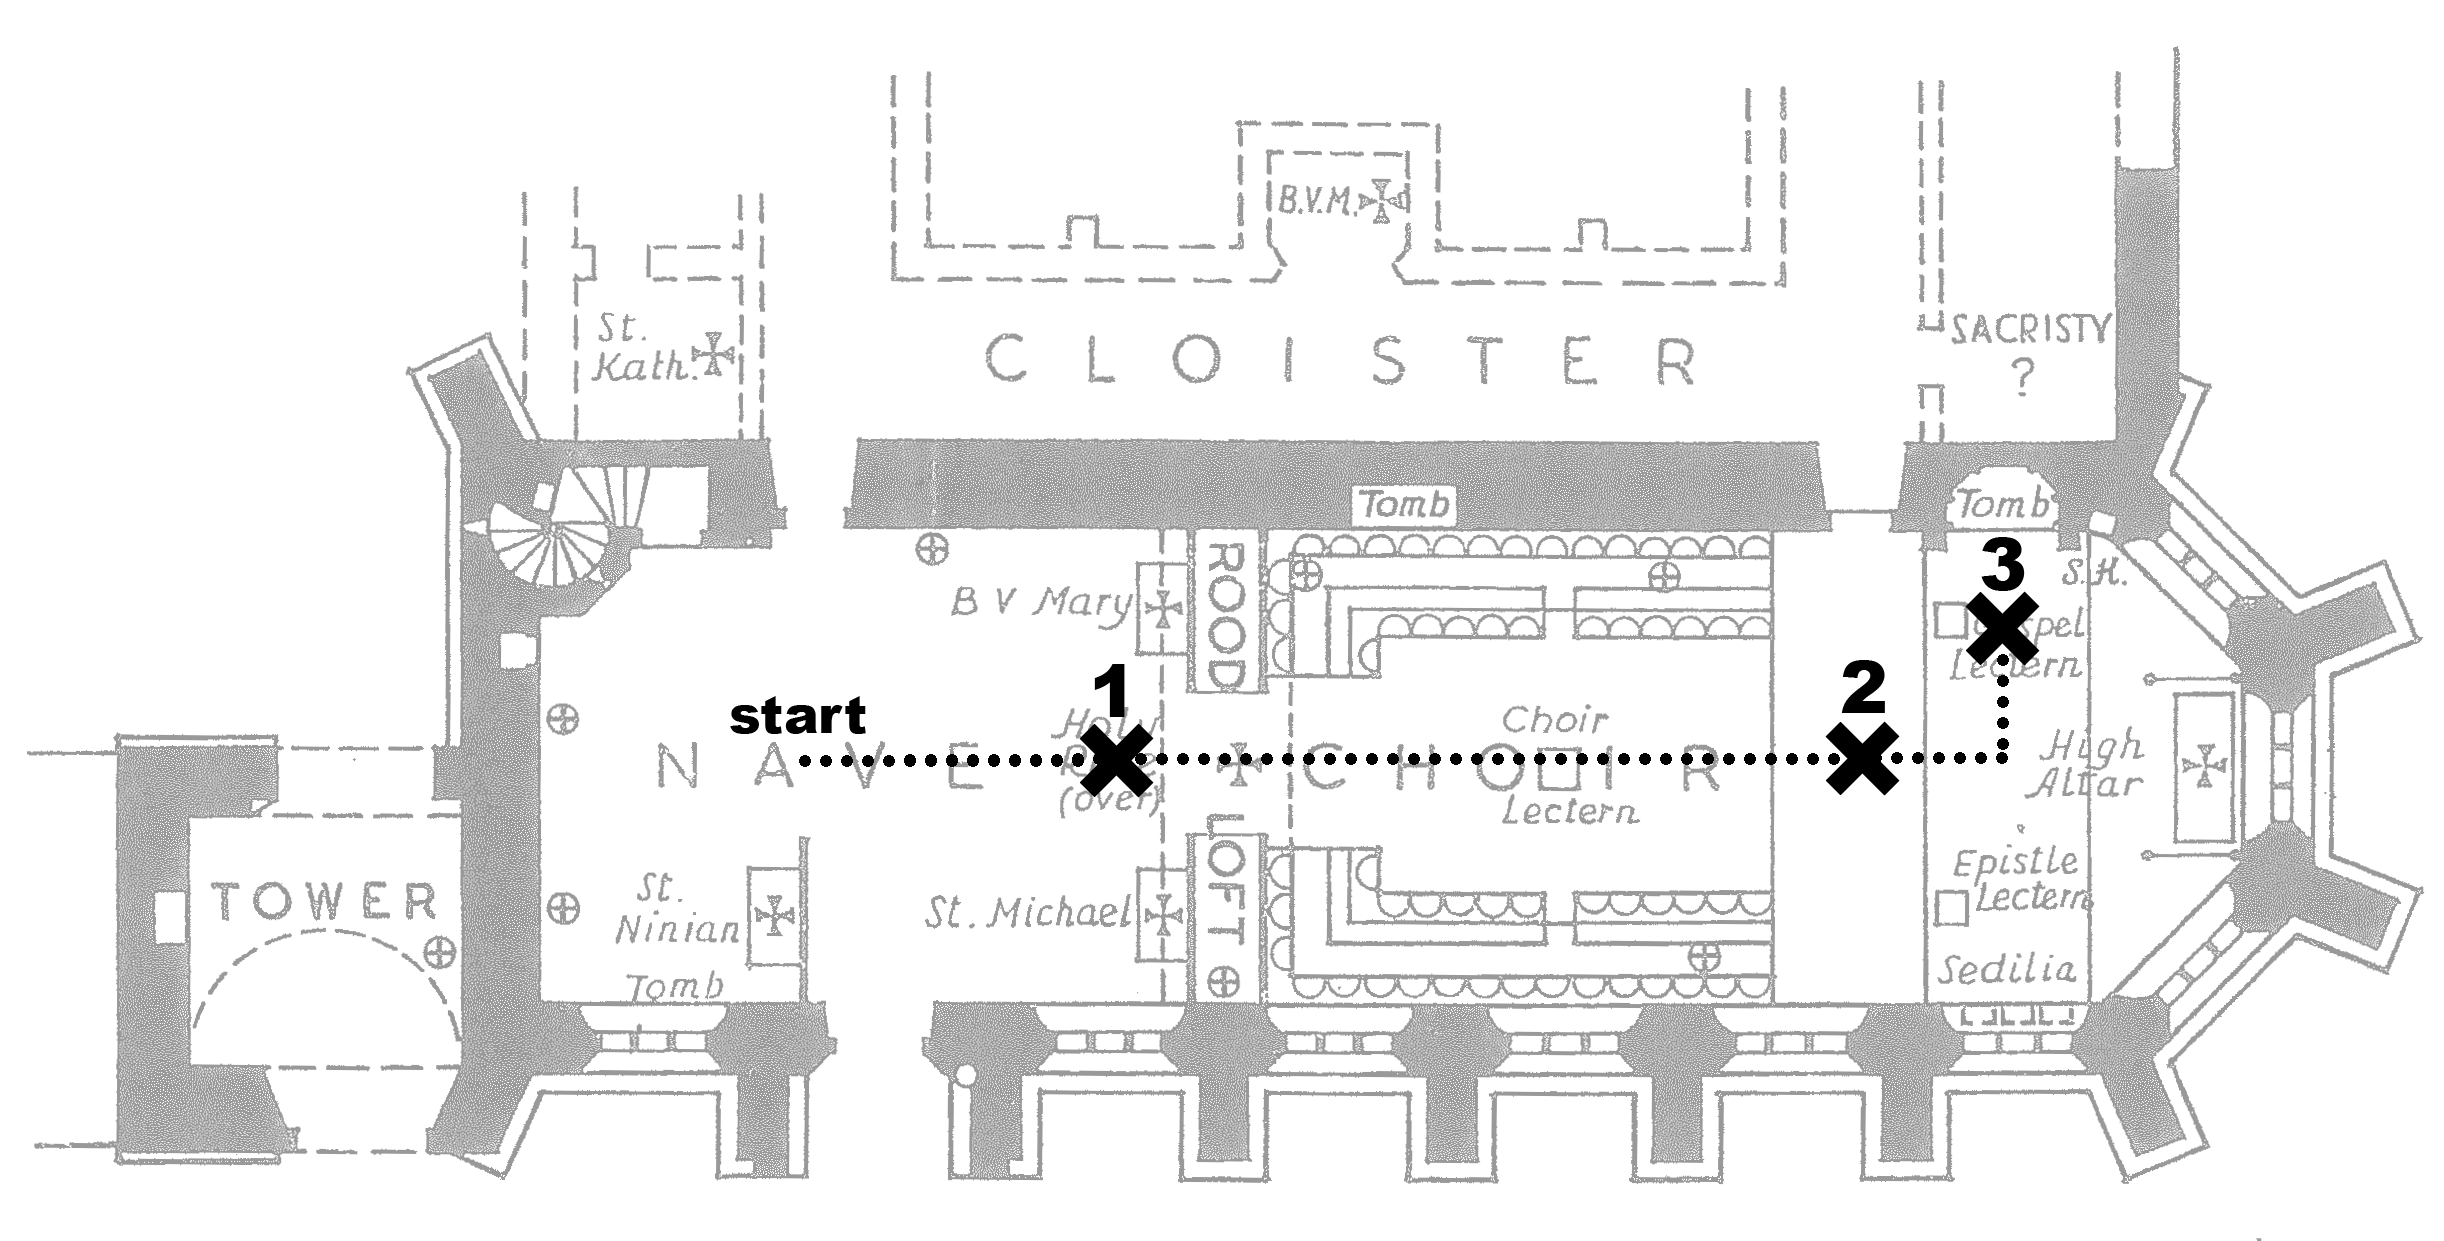
\includegraphics[width=.6\linewidth]{chapel-path.png}
		\caption{The path \& positions within the chapel that participants are instructed to attend to.}
		\label{chapel-path}
	\end{center}
\end{figure}

In the traditional scenario, participants interacted with the VR chapel using the DK1 \& Xbox controller, whilst seated. After completing the path in the VR chapel, they removed the DK1 \& walked the same path in the RW chapel. This behaviour alludes to how VR has previously been applied to cultural heritage sites such as St Salvator's chapel, wherein visitors would have the opportunity to experience a CAVE or stationary HMD based reconstruction of the site either before or after having explored the RW site. In the PR scenario, participants wore the DK1, held the Xbox controller in their right hand \& the smartphone in their left, with the laptop \& control box bundle in a satchel worn over a shoulder. They then walked the same path, but this time with the ability to transition at any time between viewing the RW chapel \& the VR chapel from the same vantage point.

In the PR scenario, participants had access to a single transition style, the transition with linear interpolation (section \ref{transition-with-linear-interpolation}), triggered by pressing \& holding the \texttt{A} button on the Xbox controller. As mentioned in section \ref{initial-testing}, this transition emerged as the `favourite' during initial tests within the OVW group. As such, it was chosen as the only transition style for the PR scenario in this first stage of evaluation wherein the focus of the investigation was upon comparing the PR scenario to the traditional scenario experience \& not upon gleaning details of the merits \& drawbacks exhibited by different PR implementations. The default view on the DK1's screen was 100\% RW with the transition causing a change to 100\% VR, a situation visualised upon the combined model in figure \ref{focus-locus-sensus-with-virtuality-continuum-with-transition}.

%=========================================================================================================

\subsection{Evaluation Techniques}

The comparison of the traditional scenario against the PR scenario included collection of a variety of both qualitative \& quantitative data. All participants completed a pre-task questionnaire, which provided calibration for their responses by enquiring about age, gender identity \& most importantly any previous experience with VR hardware \& St Salvtor's chapel (either real or virtual). The System Usability Scale (SUS)~\cite{Brooke1996} was used to provide a basic comparison between the usability of the two scenarios, while a 12-item Likert-type questionnaire was used to collect opinions on more specific aspects of the experience of both scenarios. At the end of the session, participants were engaged in a short structured interview in order to allow them to elaborate upon their experience in a more free form manner. Finally, in addition to the DK1 visuals being recorded via ShadowPlay, log data was collected during both scenarios, capturing the following information to a tab separated variable (\texttt{.tsv}) file for each frame rendered to the DK1's screen;

\begin{center}
\begin{longtable}{| l | p{8cm} |}

\hline

\texttt{<frame number>} & Incremented with each frame pushed to the DK1, starting at 0 when the Unity application is fun. \\

\hline

\texttt{<timestamp>} & According to the laptop's internal clock. \\

\hline

\texttt{<original\_position>} & The position as a Unity \texttt{Vector3} where the participant begins the experiment (as reported by IndoorAtlas). \\

\hline

\texttt{<position>} & The position as a Unity \texttt{Vector3} where the participant is on this frame (as reported by IndoorAtlas). \\

\hline

\texttt{<delta\_x>} \& \texttt{<delta\_z>} & The difference in the \texttt{x} \& \texttt{z} axes between \texttt{<original\_position>} \& \texttt{<position>} on this frame. Change in elevation (\texttt{y} axis) is not recorded, as IndoorAtlas does not provide elevation data \& the area of St Salvator's chapel used throughout the studies is largely level. \\

\hline

\texttt{<left\_rotation>} \& \texttt{<right\_rotation>} & The orientations as Unity \texttt{Quaternion} of the two Unity camera game objects. The orientation of these Unity objects is tied to the orientation of the DK1, so these values represent the orientation of the participant's head on this particular frame. \\

\hline

\texttt{<base\_oapcity>} & The maximum opacity of the game objects upon which the camera feeds are rendered. This is how reduced maximum opacity (see section \ref{subsub-baseopacity}) is implemented. \\

\hline

\texttt{<left\_opacity>} \& \texttt{<right\_opacity>} & The opacity on this frame of the game objects upon which the camera feeds are rendered. \\

\hline

\texttt{<auto\_tick>} & Whether a periodic switch is in progress (see section \ref{subsub-periodic}). \\

\hline

\texttt{<auto\_duration>} \& \texttt{<auto\_spacing>} & The interval \& duration values of the periodic hard switching (if applicable). \\

\hline

\texttt{<framerate>} & An estimate of the current frame rate (frames per second). \\

\hline

\texttt{<A\_button>}, \texttt{<B\_button>} \& \texttt{<right\_trigger>} & The current values of these inputs on the Xbox controller. For the \texttt{A} \& \texttt{B} buttons this is binary, either pressed or not, while for the trigger it is a numeric value representing the amount that the trigger is being depressed. \\

\hline

\end{longtable}
\end{center}

%=========================================================================================================

\subsection{Process}

The stage 1 investigations took place as follows;

\begin{enumerate}
	\item Participants completed the pre-task questionnaire.
	
	\item Participants were given the opportunity to familiarise themselves with the DK1 by spending a few minutes interacting with Oculus' `Tuscany' demo\footnote{\url{https://share.oculus.com/app/oculus-tuscany-demo}}. This demo was developed by Oculus themselves \& is distributed with the Rift Unity integration package. It represented at the time a very polished \& stable DK1 experience, ideal for introducing inexperienced users to HMD based VR. It was thus used to give participants an opportunity to acclimatize to the Rift, in order to reduce skewing their subsequent experiences with the St Salvator's chapel model due to drastically different levels of familiarity with the DK1 between the two scenarios.
	
	\item Participants completed the traditional scenario.
	
	\item Participants completed the SUS questionnaire \& the 12-item Likert-type questionnaire for their experience with the traditional scenario.
	
	\item Participants completed the PR scenario.
	
	\item Participants completed the SUS questionnaire \& the 12-item Likert-type questionnaire for the PR scenario.
	
	\item Participants are engaged in a short structured interview.
\end{enumerate}

%=========================================================================================================

\section{Hypotheses}

\textbf{***Do I actually need to have detailed hypotheses?}

The aim of the PR scenario is to improve participant engagement with \& understanding of the relationships between the RW \& VR environments, by addressing the problems of spatial \& temporal separation inherent with the traditional scenario, by imparting upon the participant the ability to transition between equivalent vantage points within the RW \& VR environments at will.

While it was expected for participants to report that the PR scenario did indeed allow them to better compare \& contrast the RW \& VR environments, identify differences between the RW \& VR environments \& gain a better understanding of how the RW \& VR environments relate to each other, it was expected that some participants would report that having to `split' their attention between the two environments in the PR scenario led to lessened engagement \& understanding \& that the visual quality of the RW view through the cameras led to preferring to interact with the RW environment without the DK1.

It was expected that the cumbersome nature of the PR scenario in terms of the hardware that needed to be carried by the participant \& the reduced quality of viewing the RW environment via the cameras would have a noticeable effect upon participants' movement (both position \& head orientation) in the PR scenario, most likely a restriction.

Addressing these issues, such that participants don't find viewing the real through the headset to be such a reduction in quality compared to just seeing real, such that participants feel as though they can move \& look around themselves as much in the mobile scenario as in the stationary scenario \& such that participants transition between real \& virtual at any time instead of avoiding transitions in situations in which they think that they will be unpleasant/jarring, is key \& what the stage 2 investigation focused on.

%=========================================================================================================

\subsection{SUS}
SUS scores for the PR scenario are expected to average lower than those for the traditional scenario, due to the cumbersome nature of the platform when performing the mobile scenario; during the stationary scenario, participants are seated, whilst during the mobile scenario they are required to carry a satchel over one shoulder \& hold a smartphone in their left hand. Participants who are able to overcome this cumbersomeness are expected to respond more favourably to the mobile scenario than those who cannot overcome it.

\subsection{12-item Likert-type Questionnaire}
\begin{itemize}
	\item Participants will find it easier to compare \& contrast real \& virtual environments in the mobile scenario than in the stationary scenario (q2)
	\item Participants will experience a greater  sense of `being in' the virtual environment in the mobile scenario than in the stationary scenario (q4, due to physical movement/embodiment)
	\item Participants will have a greater sense of `being in the past' in the mobile scenario than in the stationary scenario (q7)
	\item Participants will maintain greater awareness of both real \& virtual environments in the mobile scenario than in the stationary scenario (q5)
	\item Participants will gain a better understanding of what the chapel was like in the past in the mobile scenario than in the stationary scenario (q12)
\end{itemize}

\subsection{Log data}
\begin{itemize}
	\item Head movement (pitch \& yaw) will be more restricted in the mobile scenario compared to the stationary scenario
	\item Aversion to looking around (even at real) when moving in the mobile scenario
	\item Head movements will be larger discrete changes in the stationary scenario compared to the mobile scenario
	\item Tendency to only look at virtual when looking around
\end{itemize}

\subsection{Interviews}
\begin{itemize}
	\item mobile scenario makes it easier to spot differences
	\item mobile scenario reveals differences that stationary didn't
	\item stationary does not reveal differences that mobile doesn't
	\item mobile scenario is preferred \& is user-reported as 'more engaging'
\end{itemize}

%=========================================================================================================

\section{Stage 1 Results}

A total of 6 participants completed the stage 1 investigation, however due to a mistake only 5 participants completed the 12-item Likert-type questionnaires correctly.

For n = 6
\begin{itemize}
	\item age ranged from 21 to 26, mean age 23.3, sd 1.86
	\item 3x identified as male \& 3x as female
	\item all reported previous experience with a games console controller
	\item 1x reported previous experience with a HMD
	\item 2x reported having previously visited the chapel
	\item none had previously experienced the virtual chapel
\end{itemize}

For n = 5 (excluding the participant who did not complete the 12-item Likert-type questionnaires correctly);
\begin{itemize}
	\item age ranged from 21 to 26, mean age 23, sd 1.87
	\item 3x identified as male \& 2x as female
	\item all reported previous experience with a games console controller
	\item none reported previous experience with a HMD
	\item 1x reported having previously visited the chapel
	\item none had previously experienced the virtual chapel
\end{itemize}

\TwoFig{1/sus.png}{SUS results.}{sus.png}
       {1/post_task_questionnaire_boxplot.png}{12-item questionnaire results.}{post_task_questionnaire_boxplot.png}










%=========================================================================================================

\subsection{Pre-task Questionnaire}

For n=5 ages ranged from 21-26, 3x female \& 2x male, all reported previous experience using a games console controller, 1x reported previous use of a HMD, 2x reported having previously visited the chapel, none had previously interacted with the virtual chapel model.

\subsection{SUS}


As expected, the SUS scores for the mobile scenario are lower than those of the stationary scenario, although not drastically so. Furthermore, although scoring lower on SUS, the mobile scenario came out above the stationary scenario when looking at the results of q8 in the 12-item questionnaire which asked participants if they thought they would have preferred a conventional computer monitor.

\subsection{12-item Questionnaire}


The hypotheses seem to hold, in particular;

\begin{itemize}
	\item \textit{Participants will maintain greater awareness of both real \& virtual environments in the mobile scenario than in the stationary scenario} is supported by the responses to q5
	\item \textit{Participants will have a greater sense of `being in the past' in the mobile scenario than in the stationary scenario} is supported by q7 (thanks to embodiment?)
	\item \textit{Participants will gain a better understanding of what the chapel was like in the past in the mobile scenario than in the stationary scenario} is supported by q12
\end{itemize}

It is worth highlighting the responses to q10 in relation to those to q2. Participants reported finding it easier to compare features from the past \& present (q2) during the mobile scenario, however did not report a difference between not noticing differences between the real \& virtual environments (q10).

%=========================================================================================================

%\makebox[\textwidth][c]{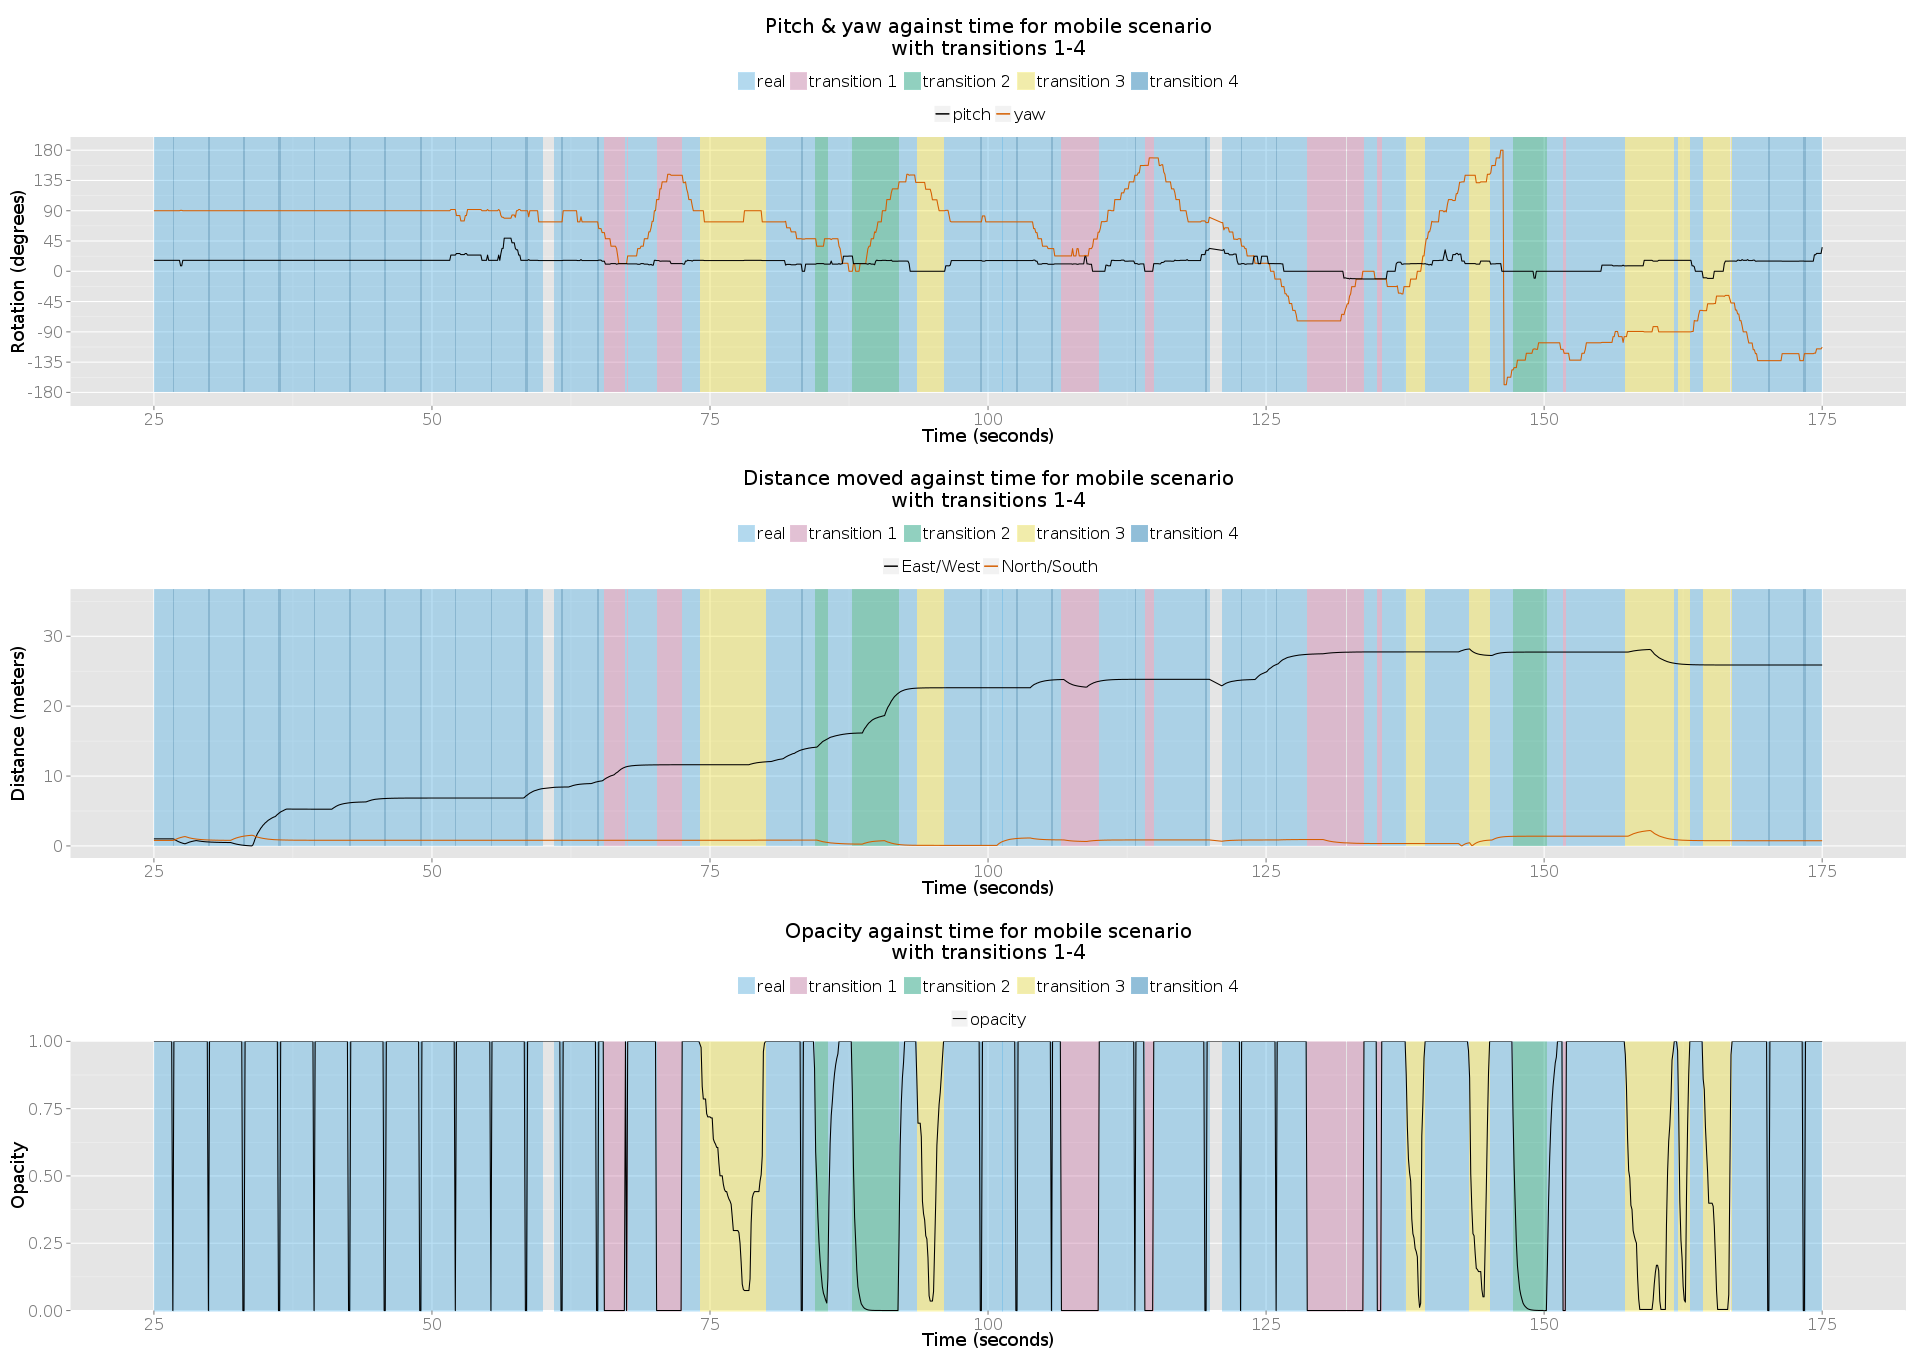
\includegraphics[width=1.2\textwidth]{2.1/11_1-4_3up.png}}

\clearpage

\subsection{Participant 1}

\begin{figure}[h]
	\begin{center}
	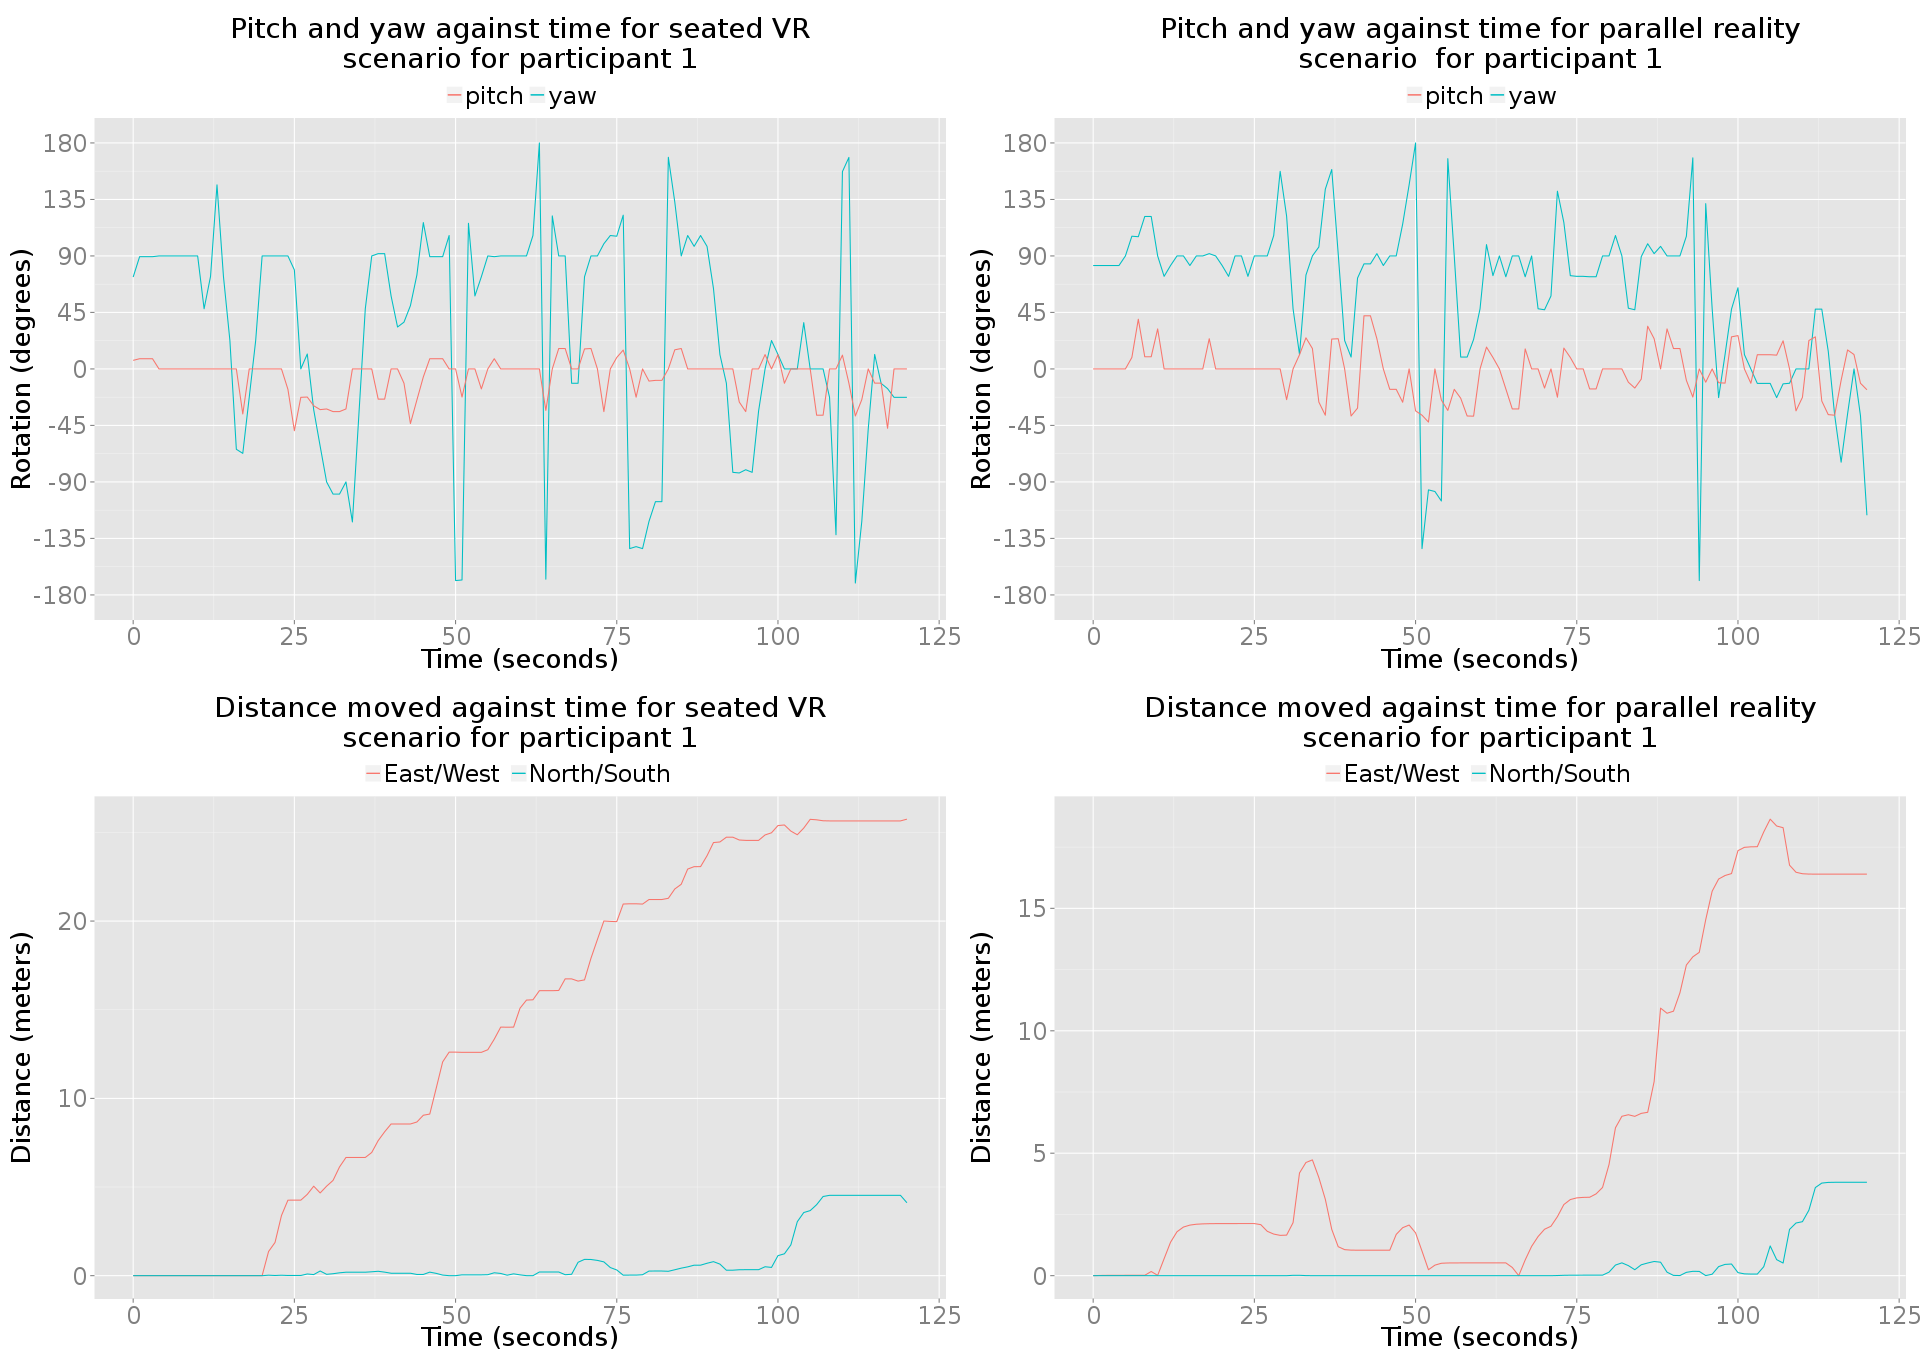
\includegraphics[width=\textwidth]{1/1_4up.png}
	\caption{Some images, yah.}
	\end{center}
\end{figure}

\clearpage

\begin{figure}[h]
	\begin{center}
	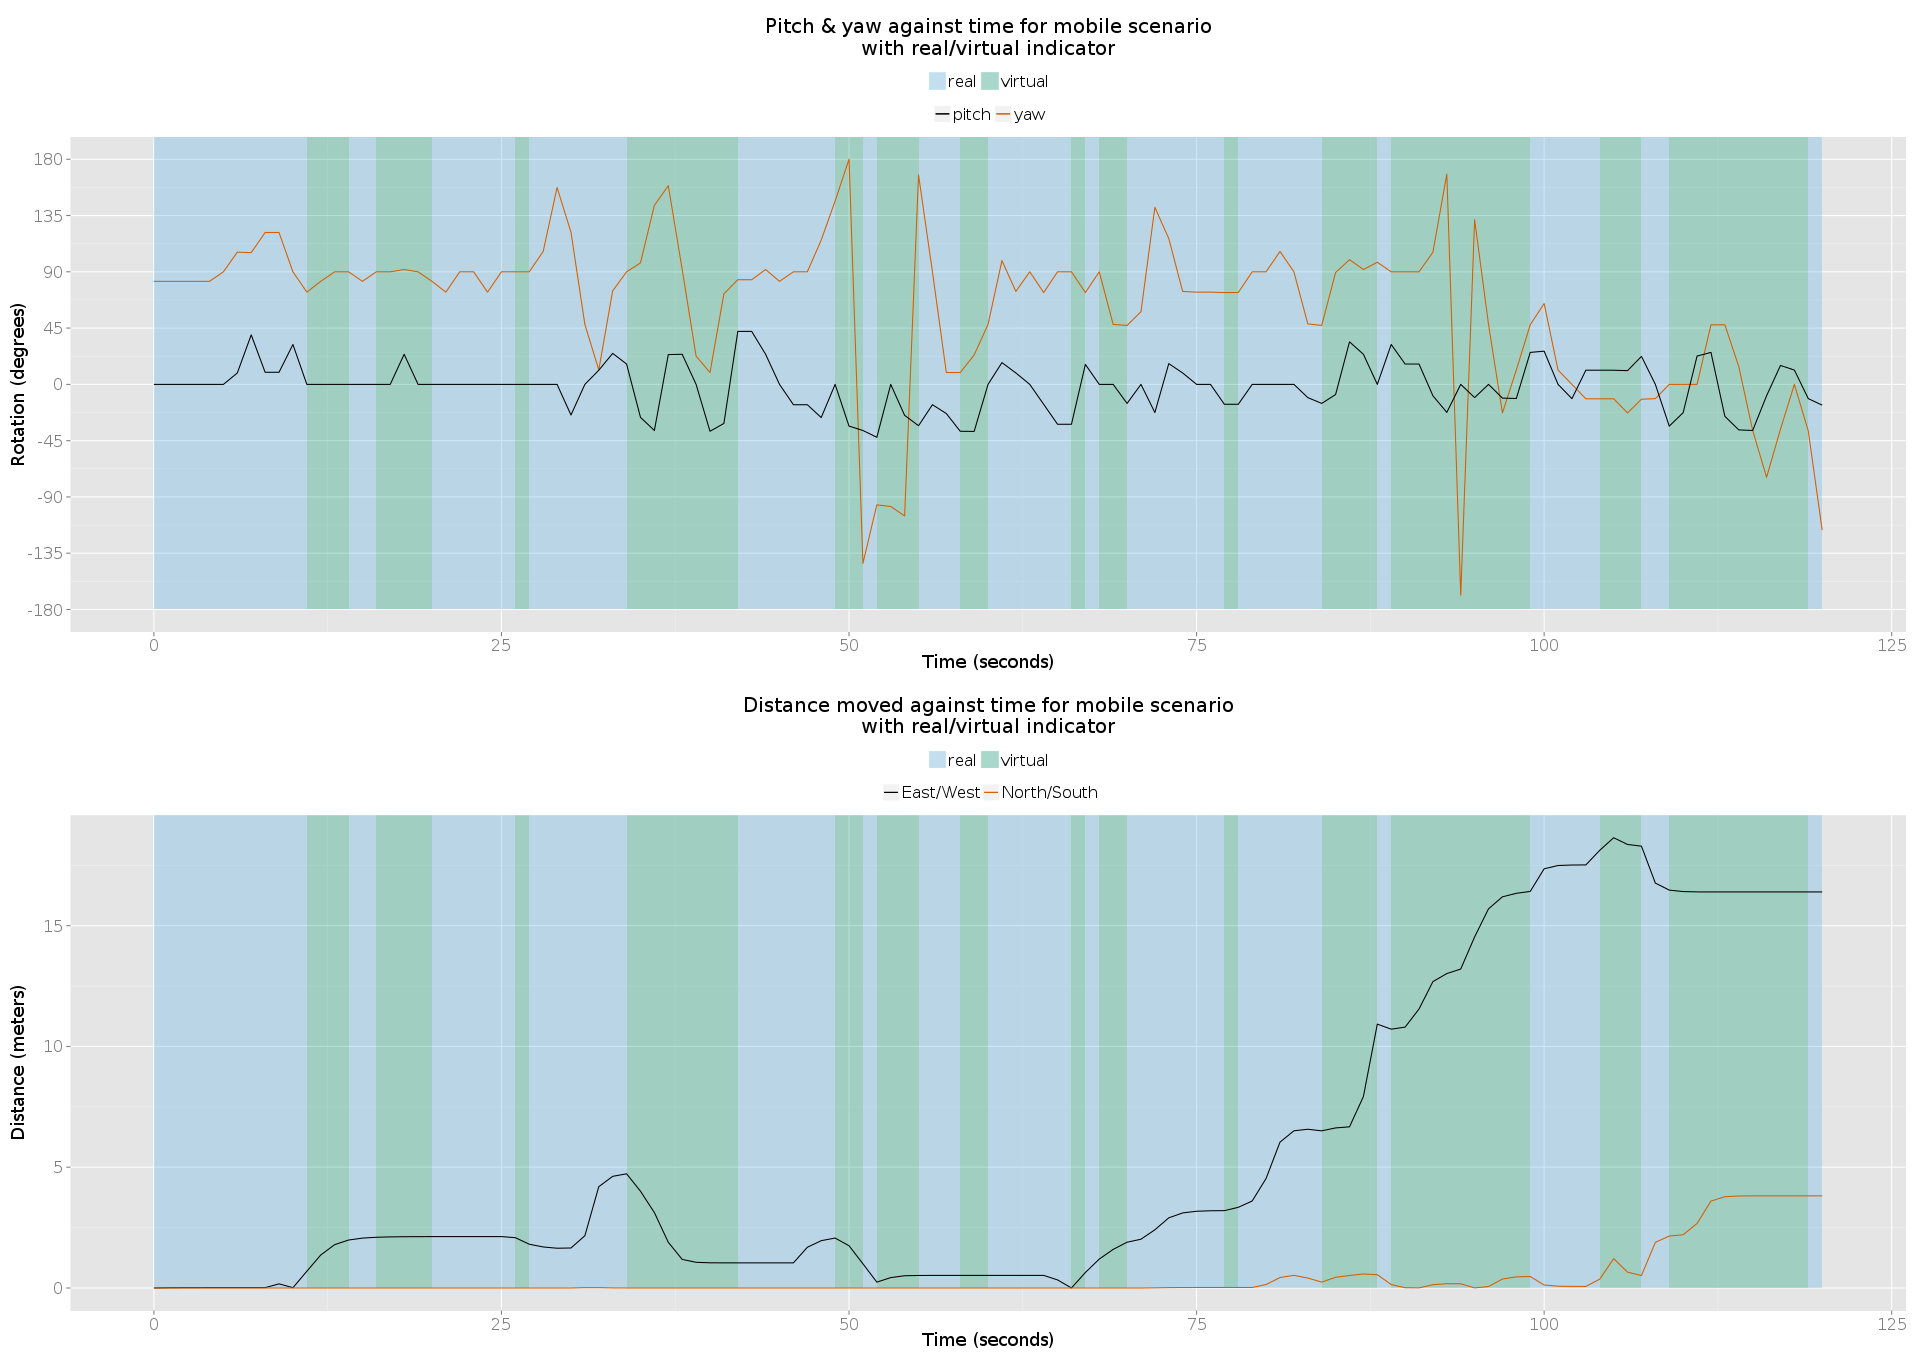
\includegraphics[width=\textwidth]{1/1_2up.png}
	\caption{Some images, yah.}
	\end{center}
\end{figure}

%=========================================================================================================

\clearpage

\subsection{Participant 3}

\begin{figure}[h]
	\begin{center}
	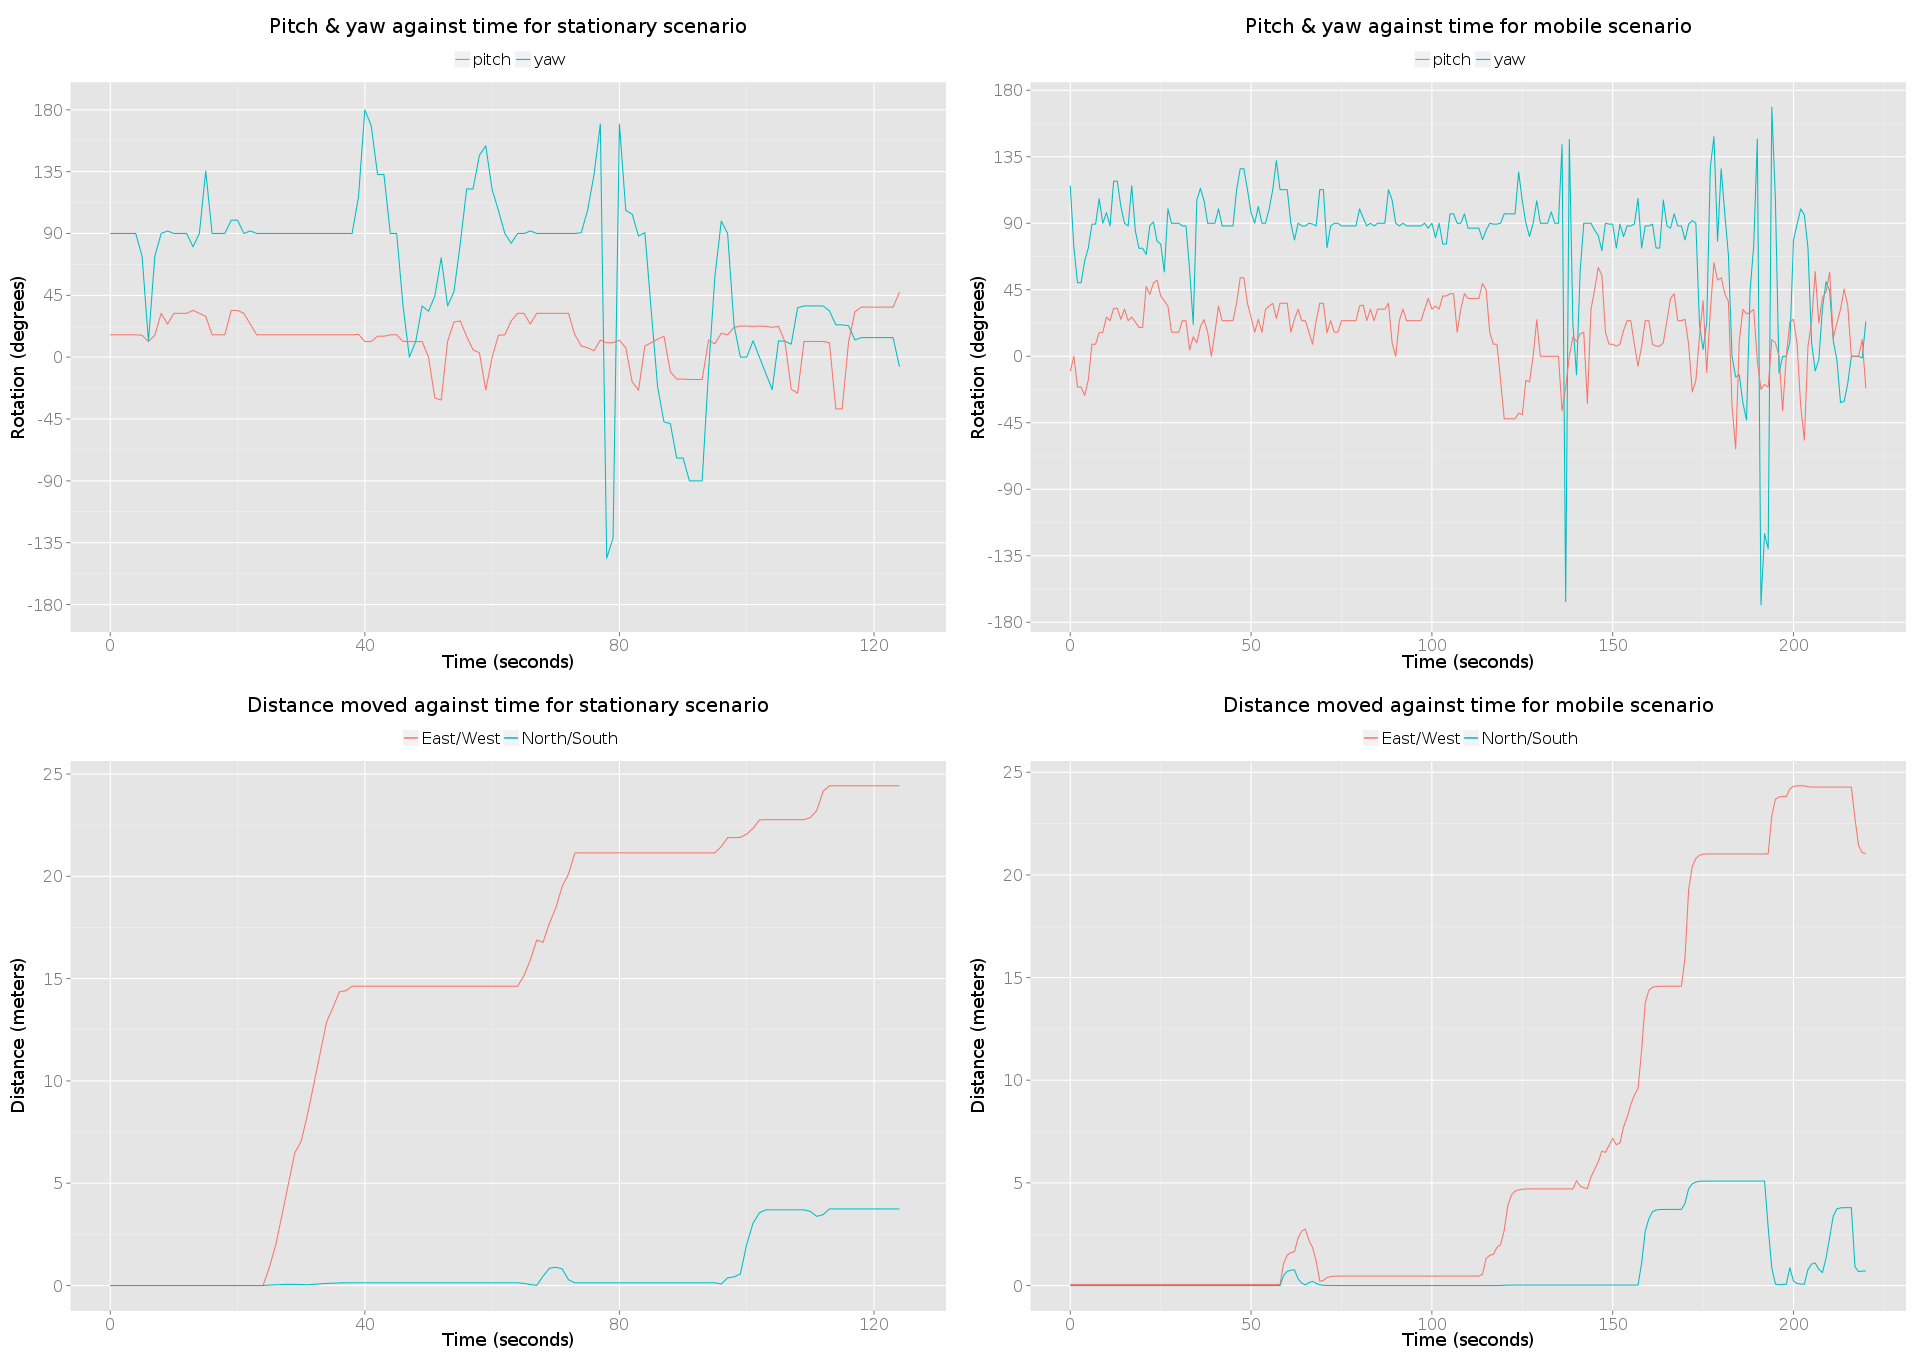
\includegraphics[width=\textwidth]{1/3_4up.png}
	\caption{Some images, yah.}
	\end{center}
\end{figure}

\clearpage

\begin{figure}[h]
	\begin{center}
	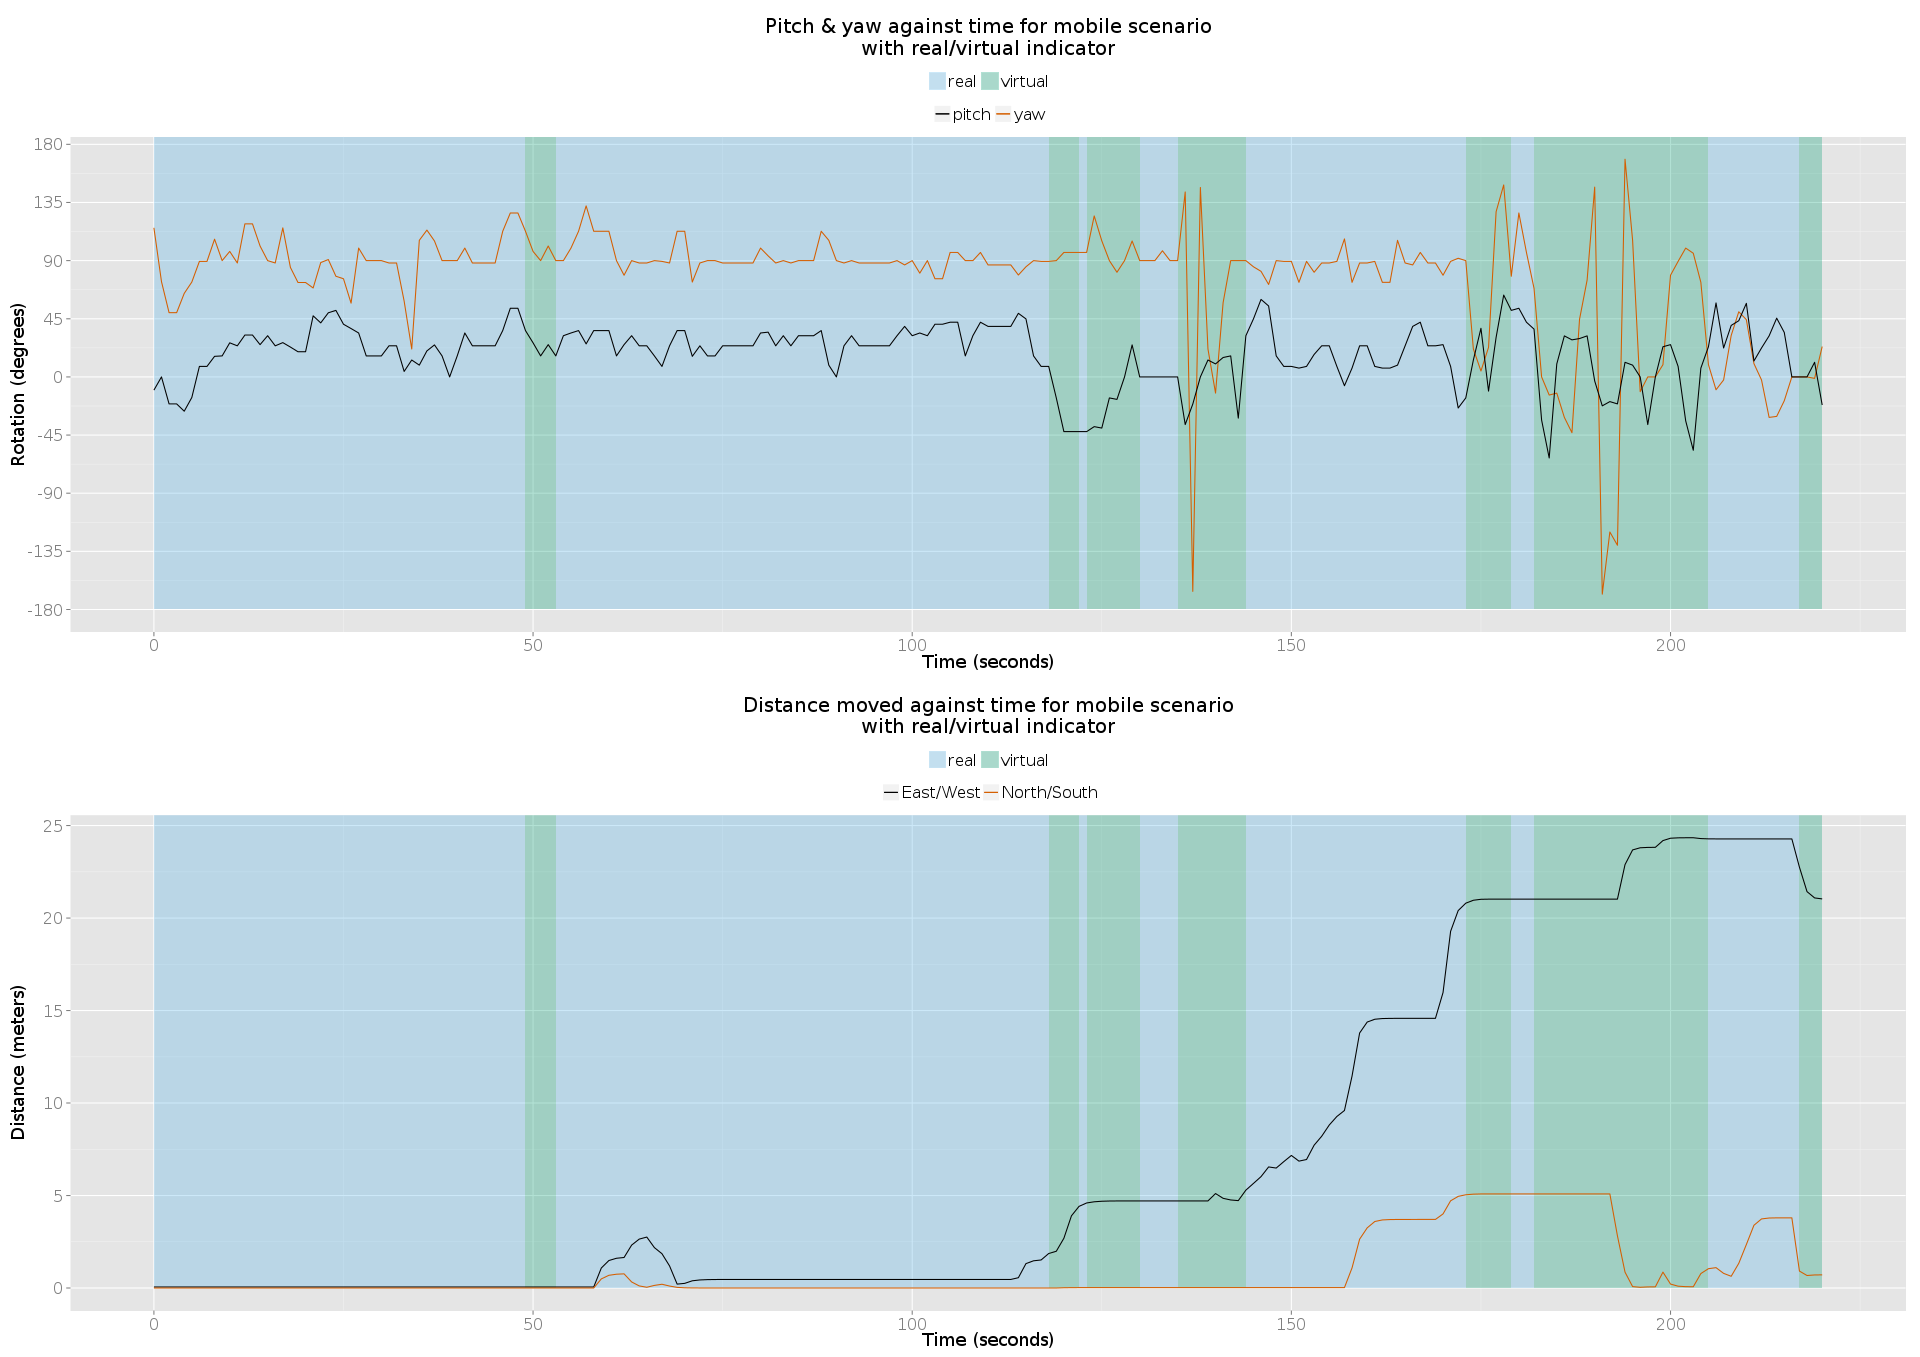
\includegraphics[width=\textwidth]{1/3_2up.png}
	\caption{Some images, yah.}
	\end{center}
\end{figure}

%=========================================================================================================

\clearpage

\subsection{Participant 4}

\begin{figure}[h]
	\begin{center}
	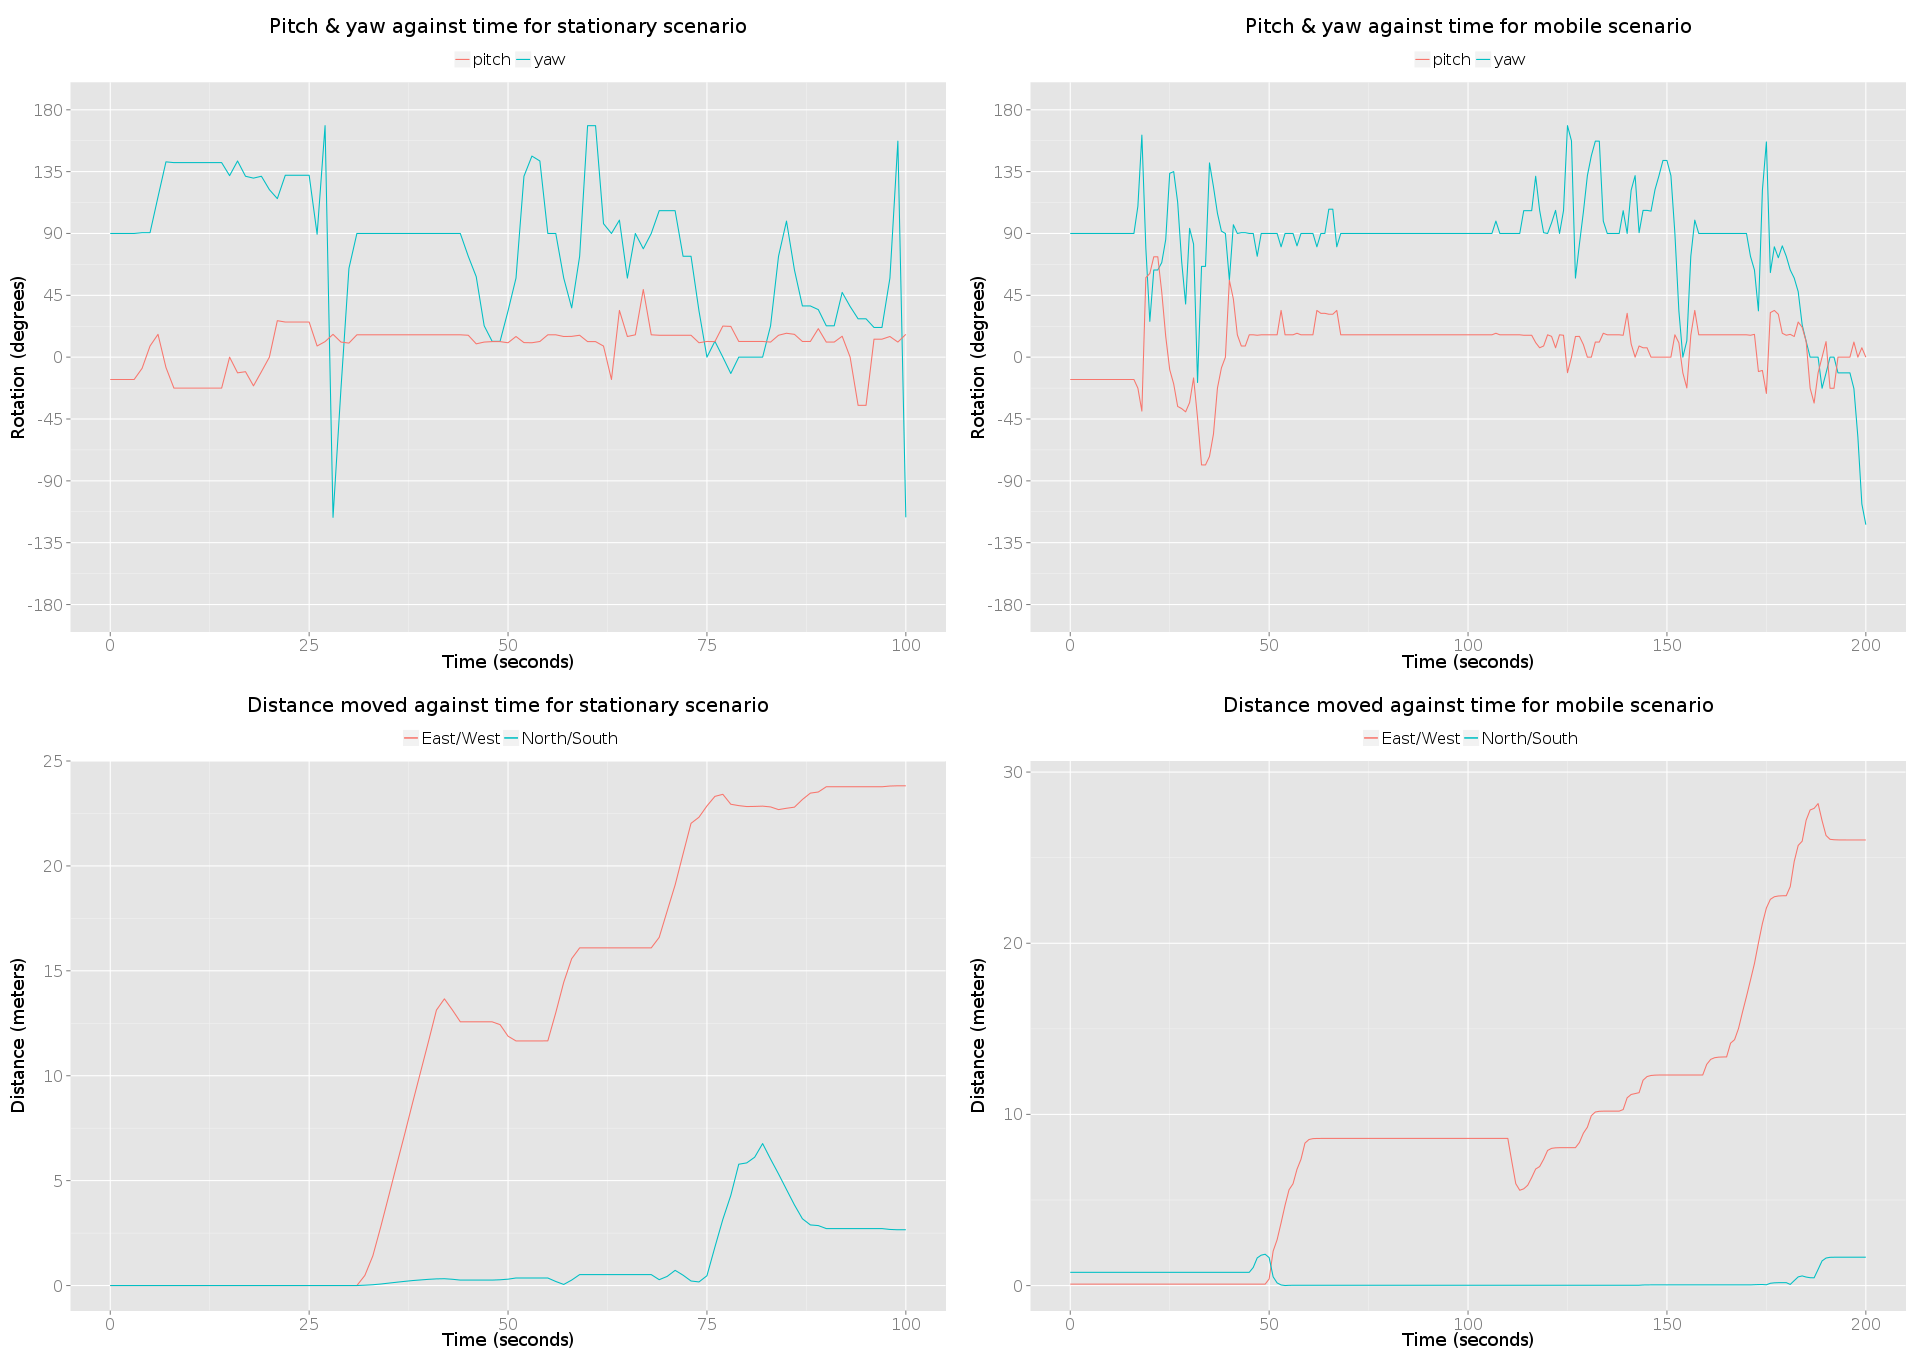
\includegraphics[width=\textwidth]{1/4_4up.png}
	\caption{Some images, yah.}
	\end{center}
\end{figure}

\clearpage

\begin{figure}[h]
	\begin{center}
	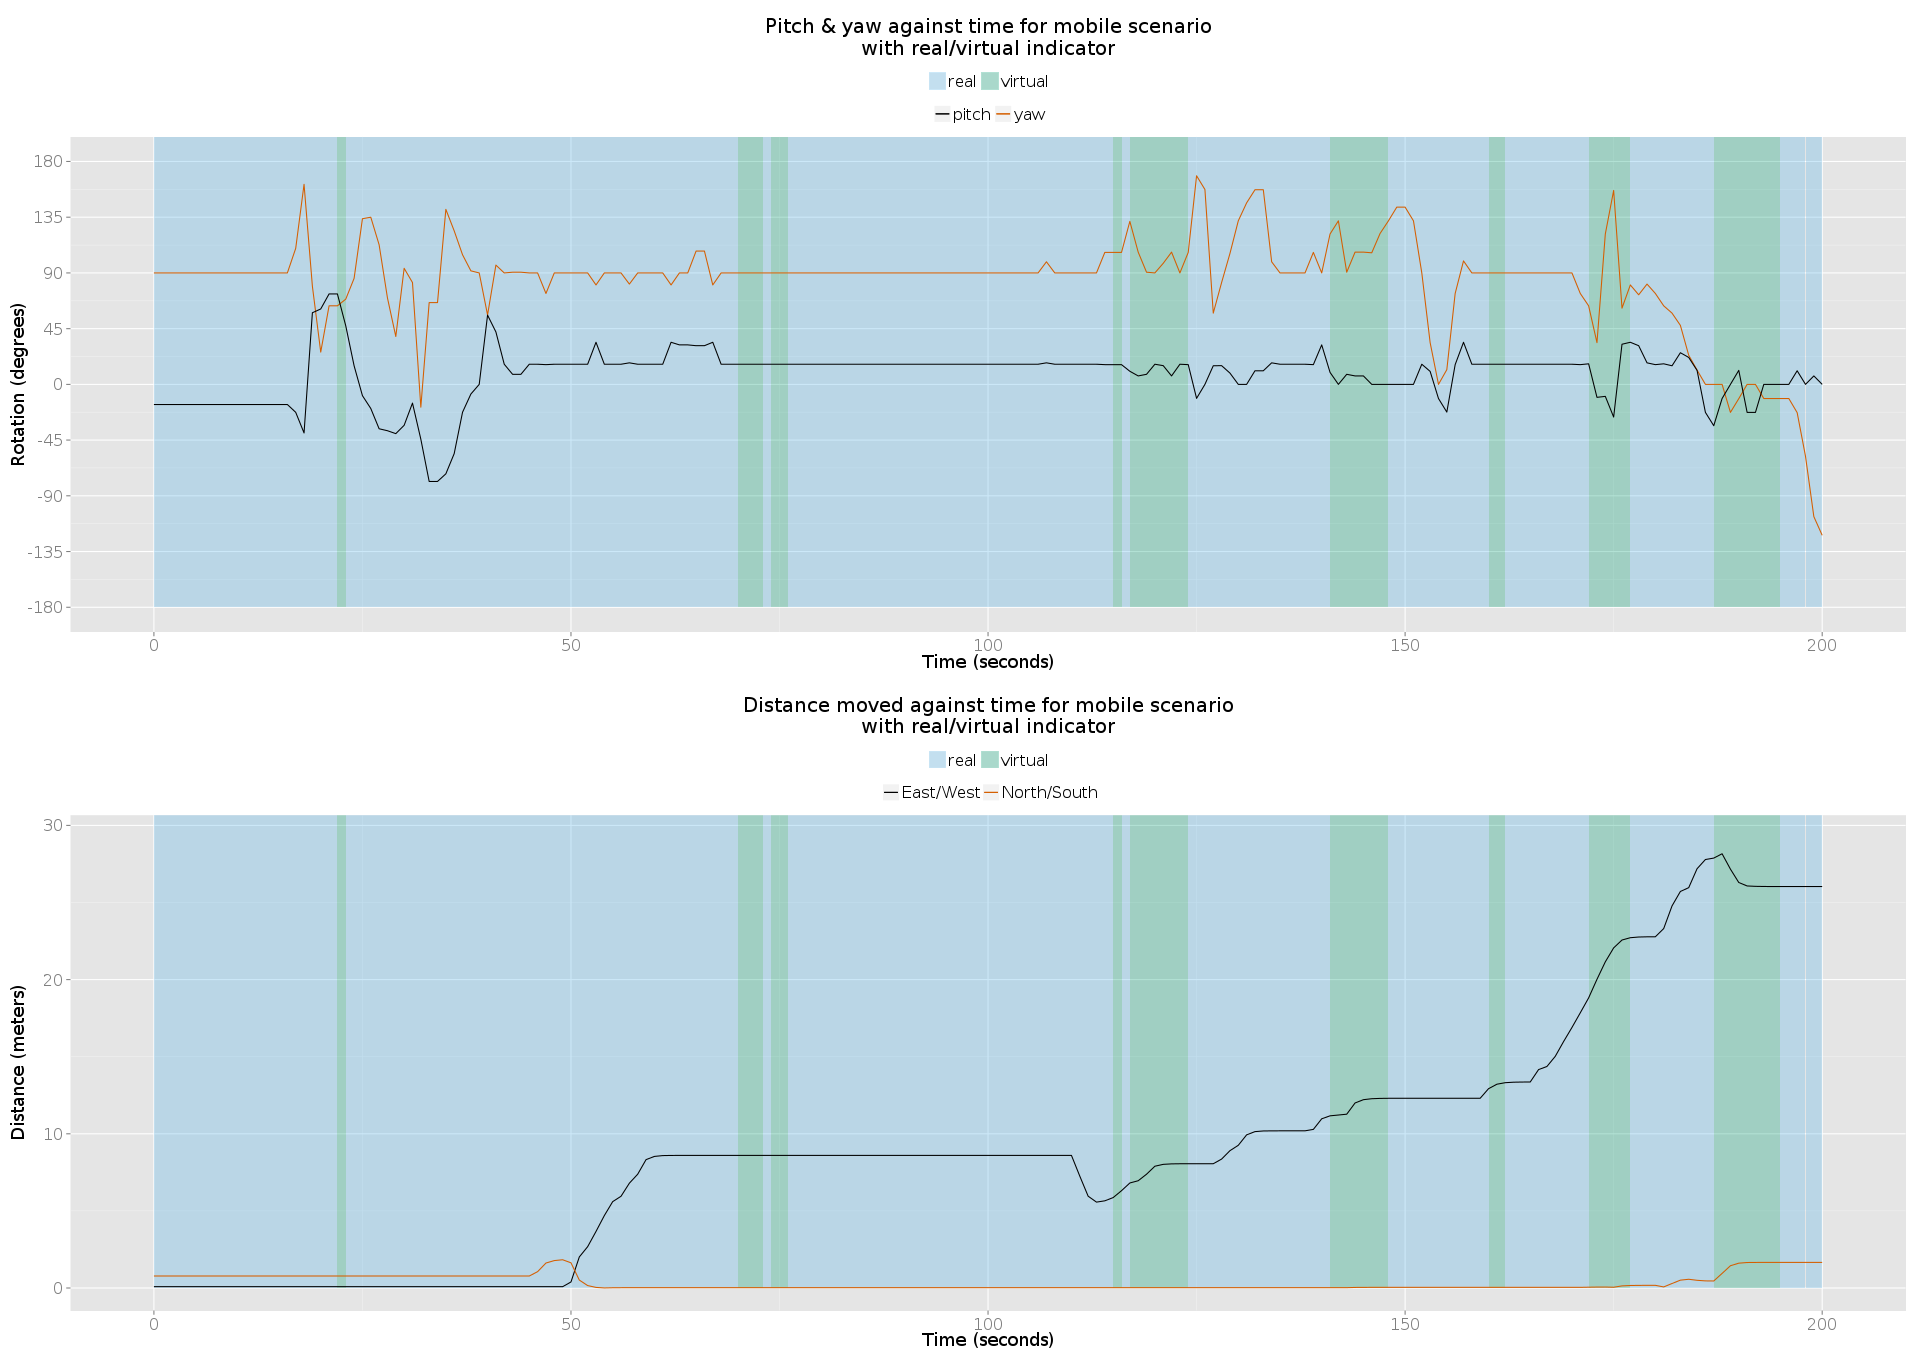
\includegraphics[width=\textwidth]{1/4_2up.png}
	\caption{Some images, yah.}
	\end{center}
\end{figure}

%=========================================================================================================

\subsection{Participant 5}

\clearpage

\begin{figure}[h]
	\begin{center}
	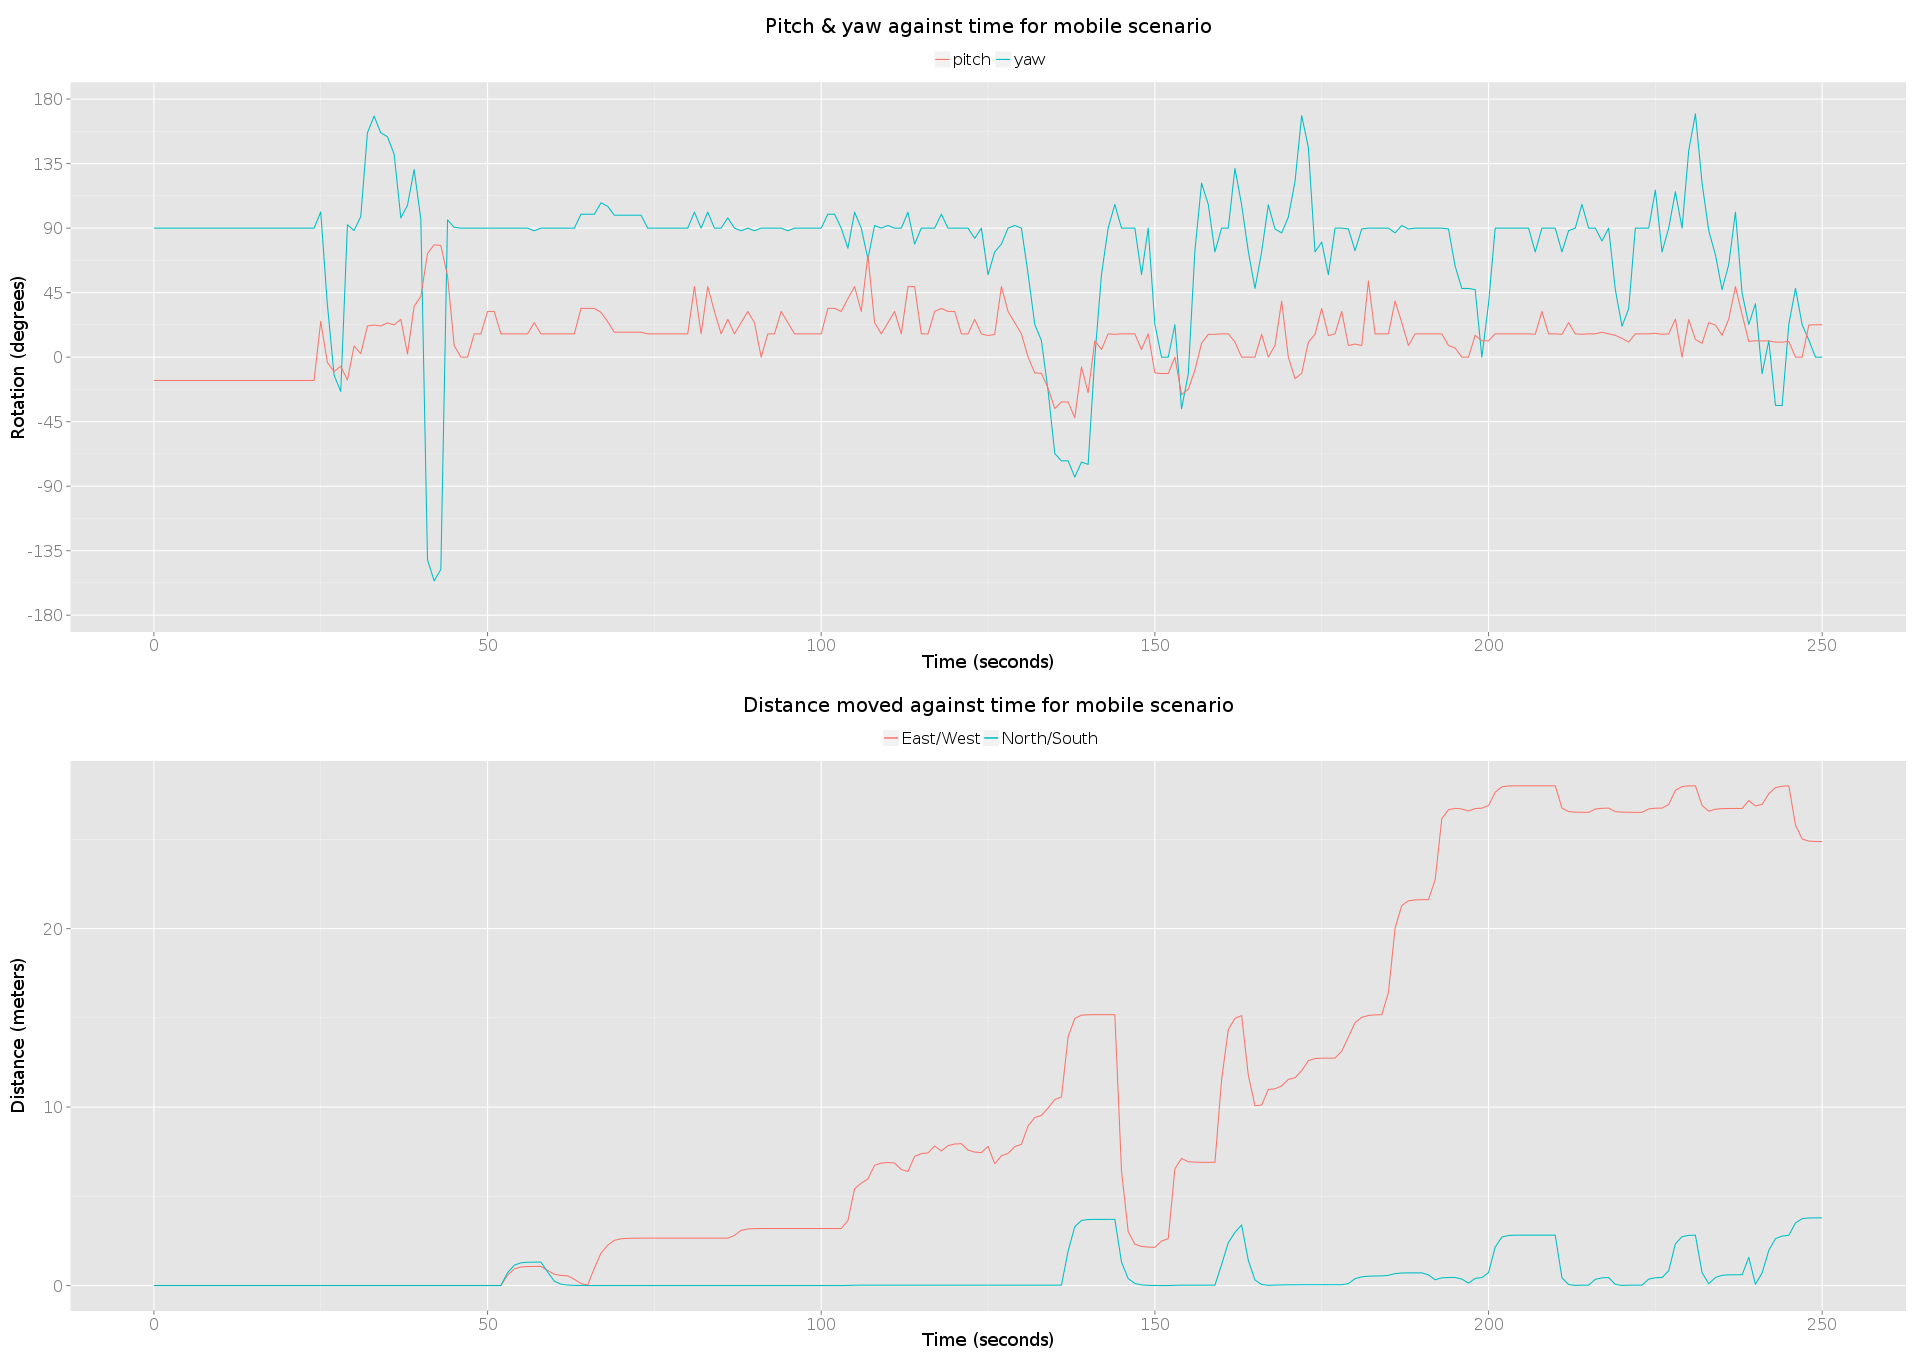
\includegraphics[width=\textwidth]{1/5_4up.png}
	\caption{Some images, yah.}
	\end{center}
\end{figure}

\clearpage

\begin{figure}[h]
	\begin{center}
	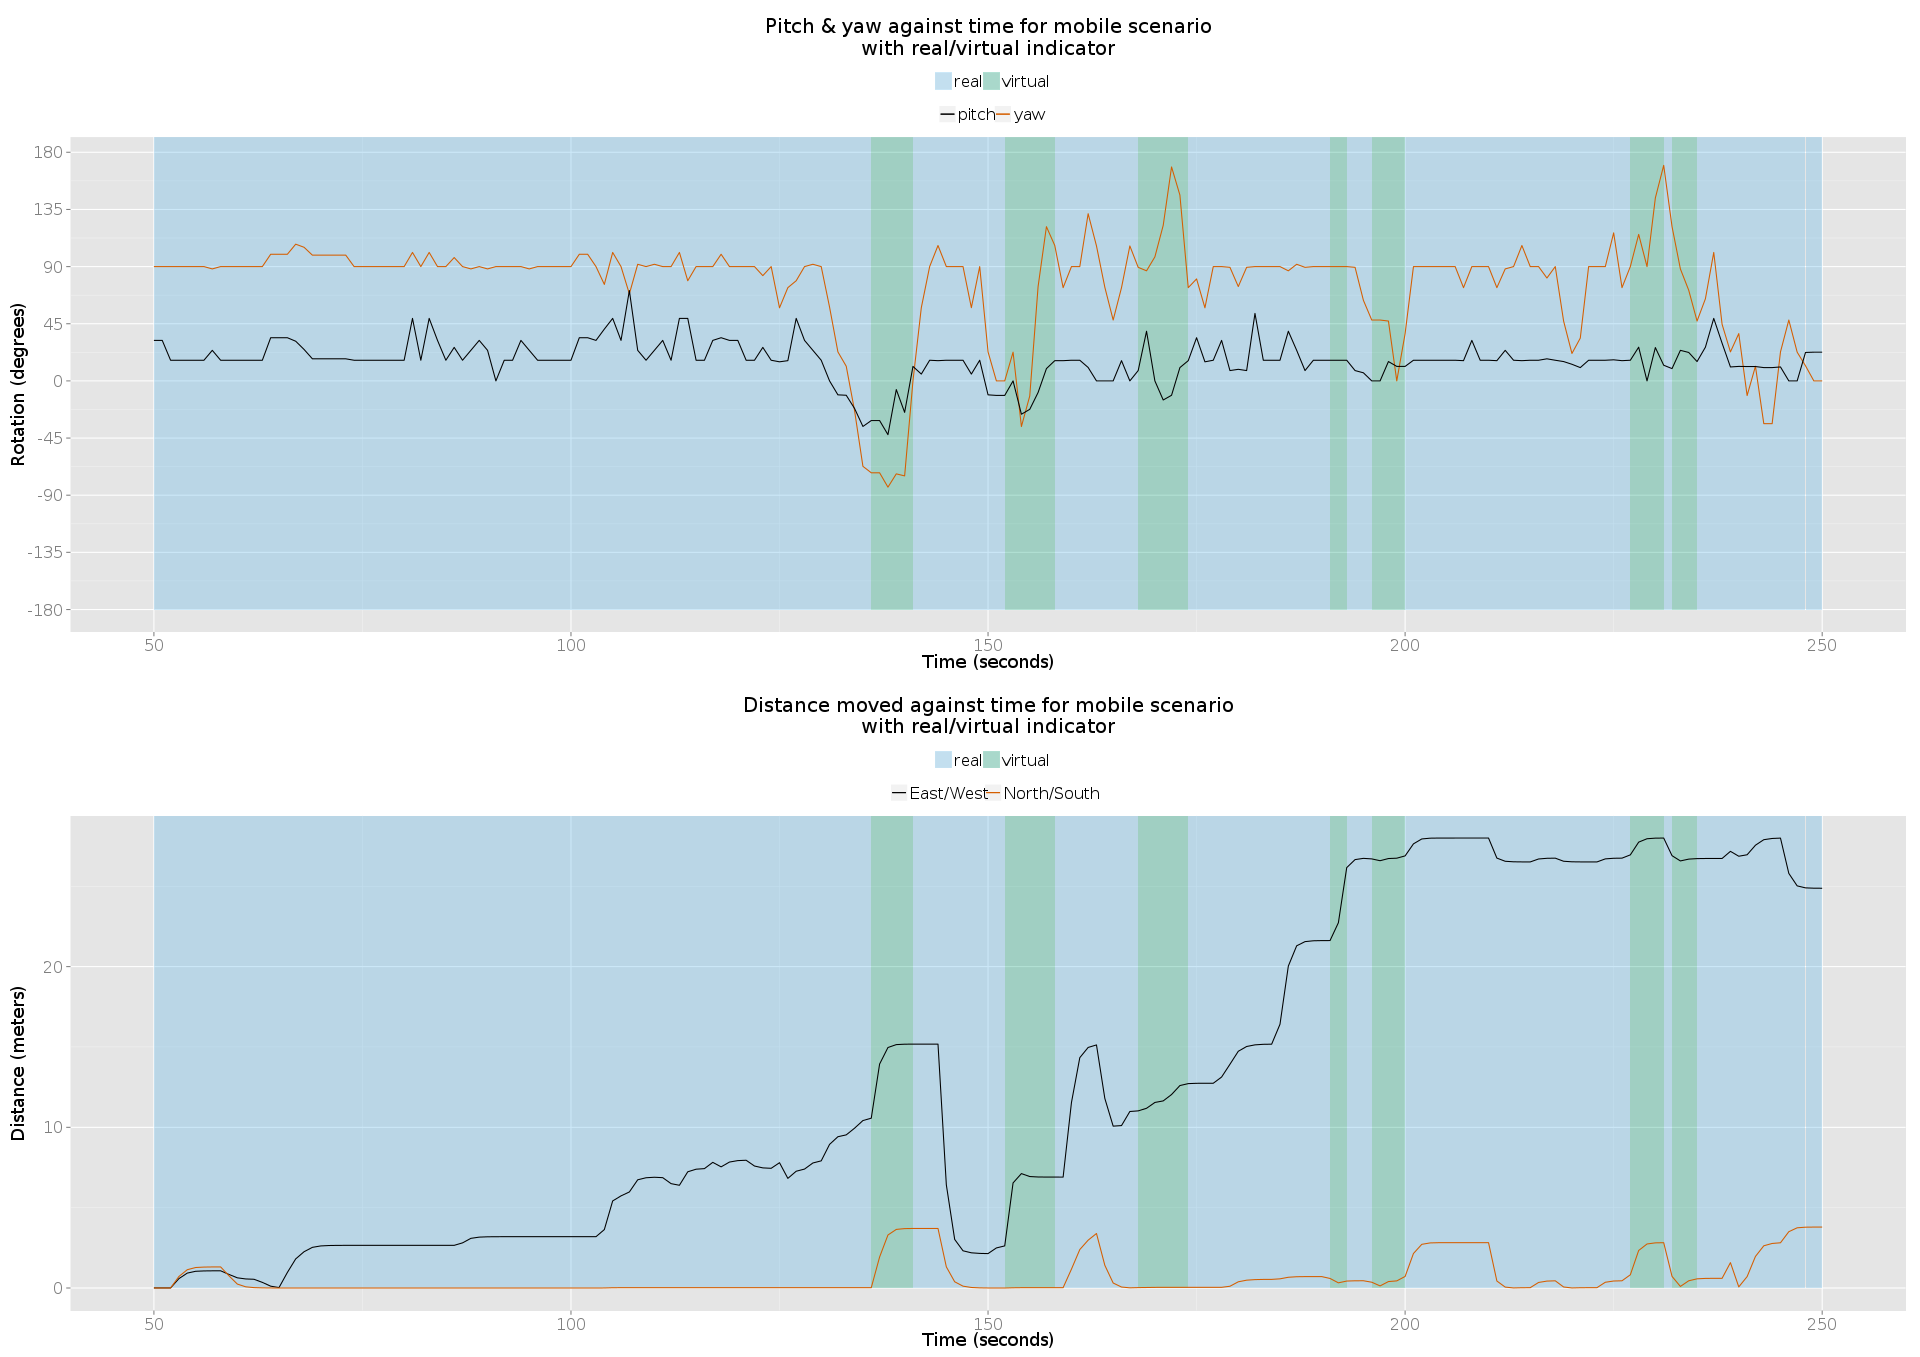
\includegraphics[width=\textwidth]{1/5_2up.png}
	\caption{Some images, yah.}
	\end{center}
\end{figure}

%=========================================================================================================

\subsection{Participant 6}

\clearpage

\begin{figure}[h]
	\begin{center}
	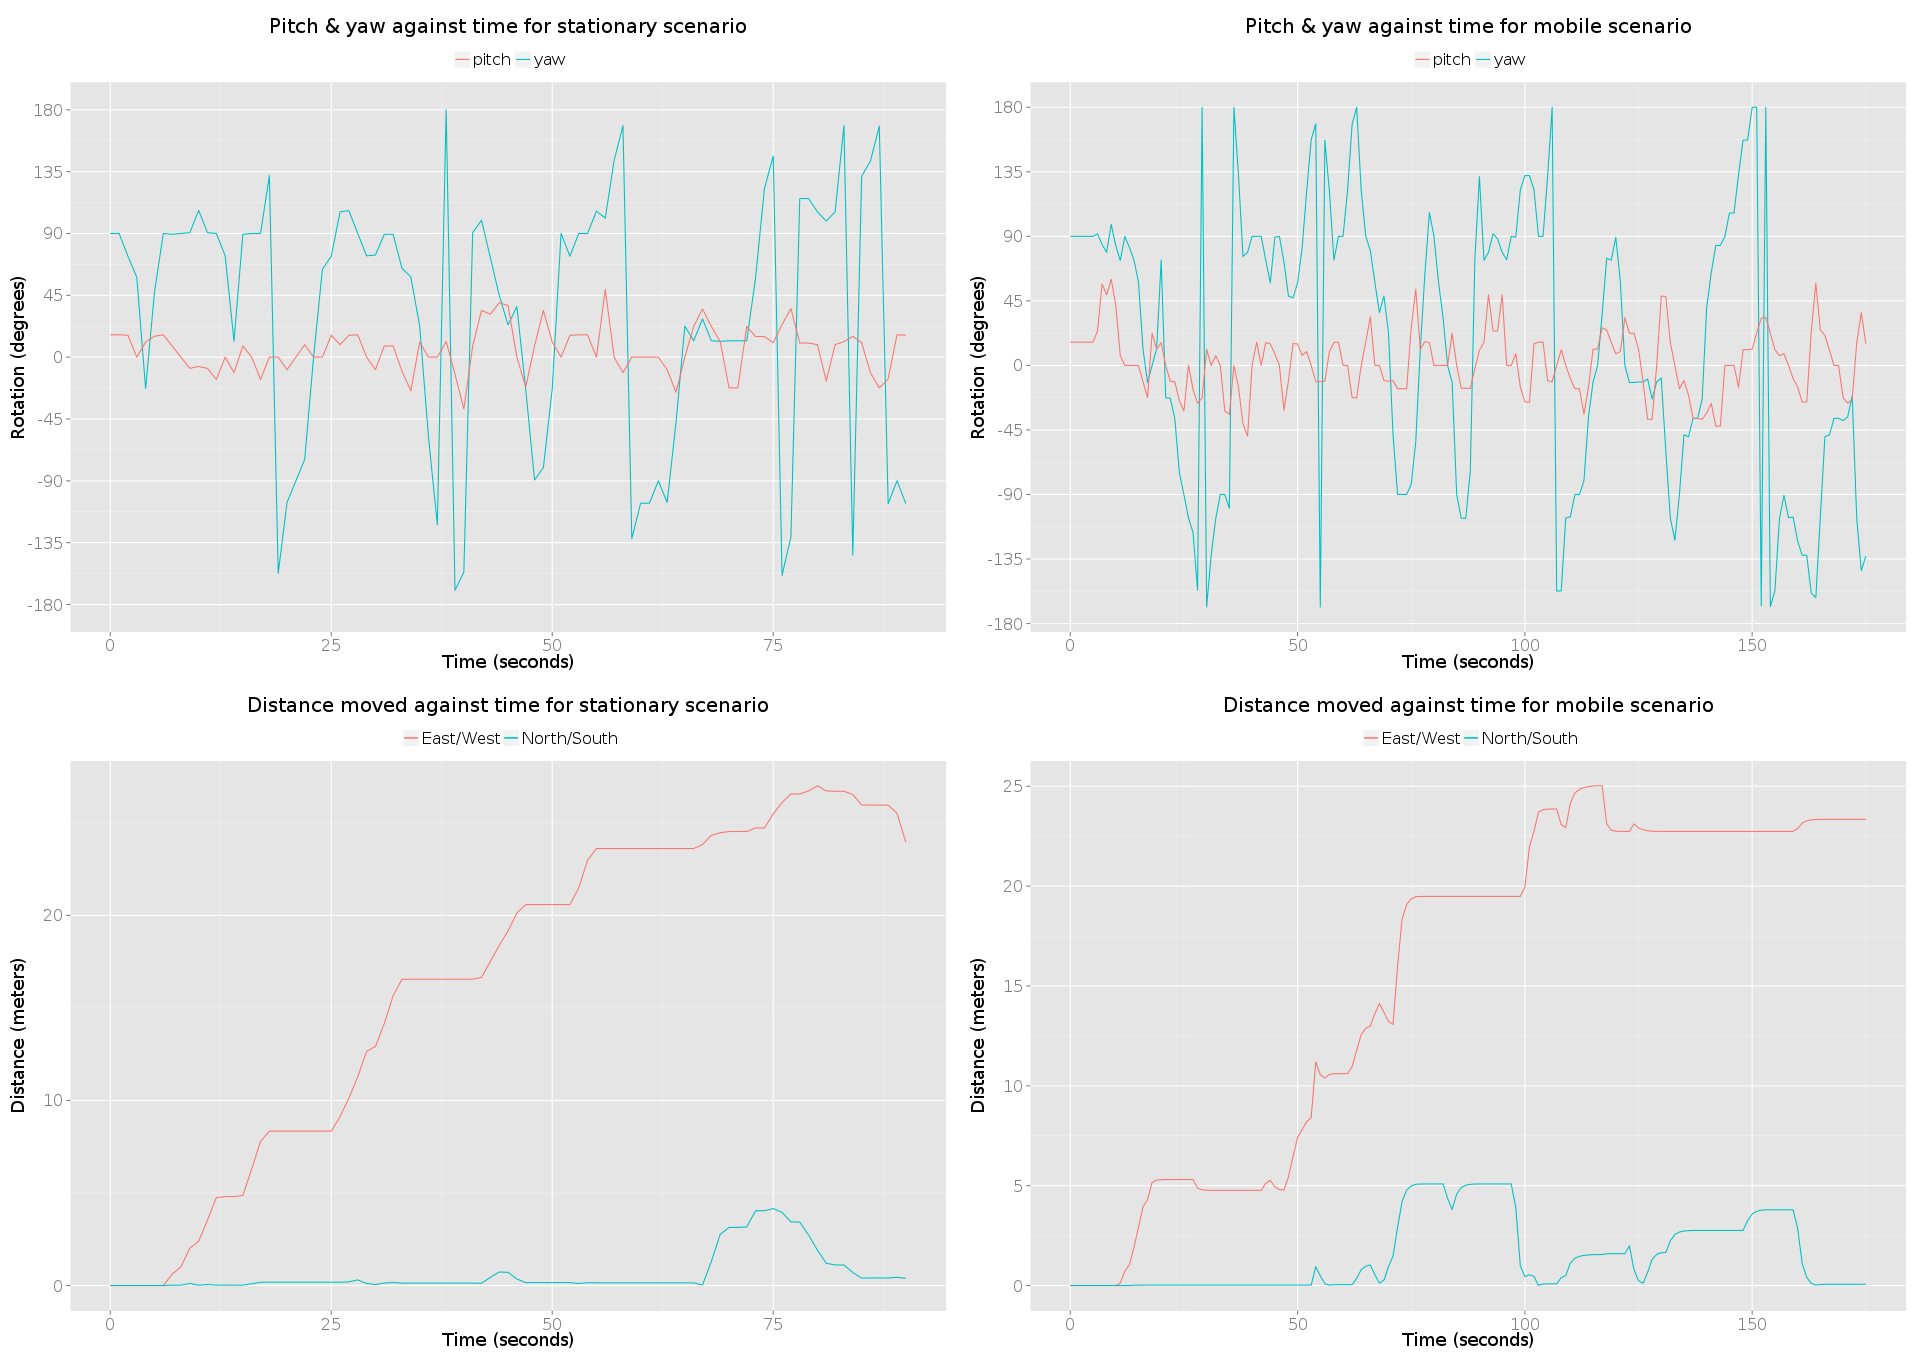
\includegraphics[width=\textwidth]{1/6_4up.png}
	\caption{Some images, yah.}
	\end{center}
\end{figure}

\clearpage

\begin{figure}[h]
	\begin{center}
	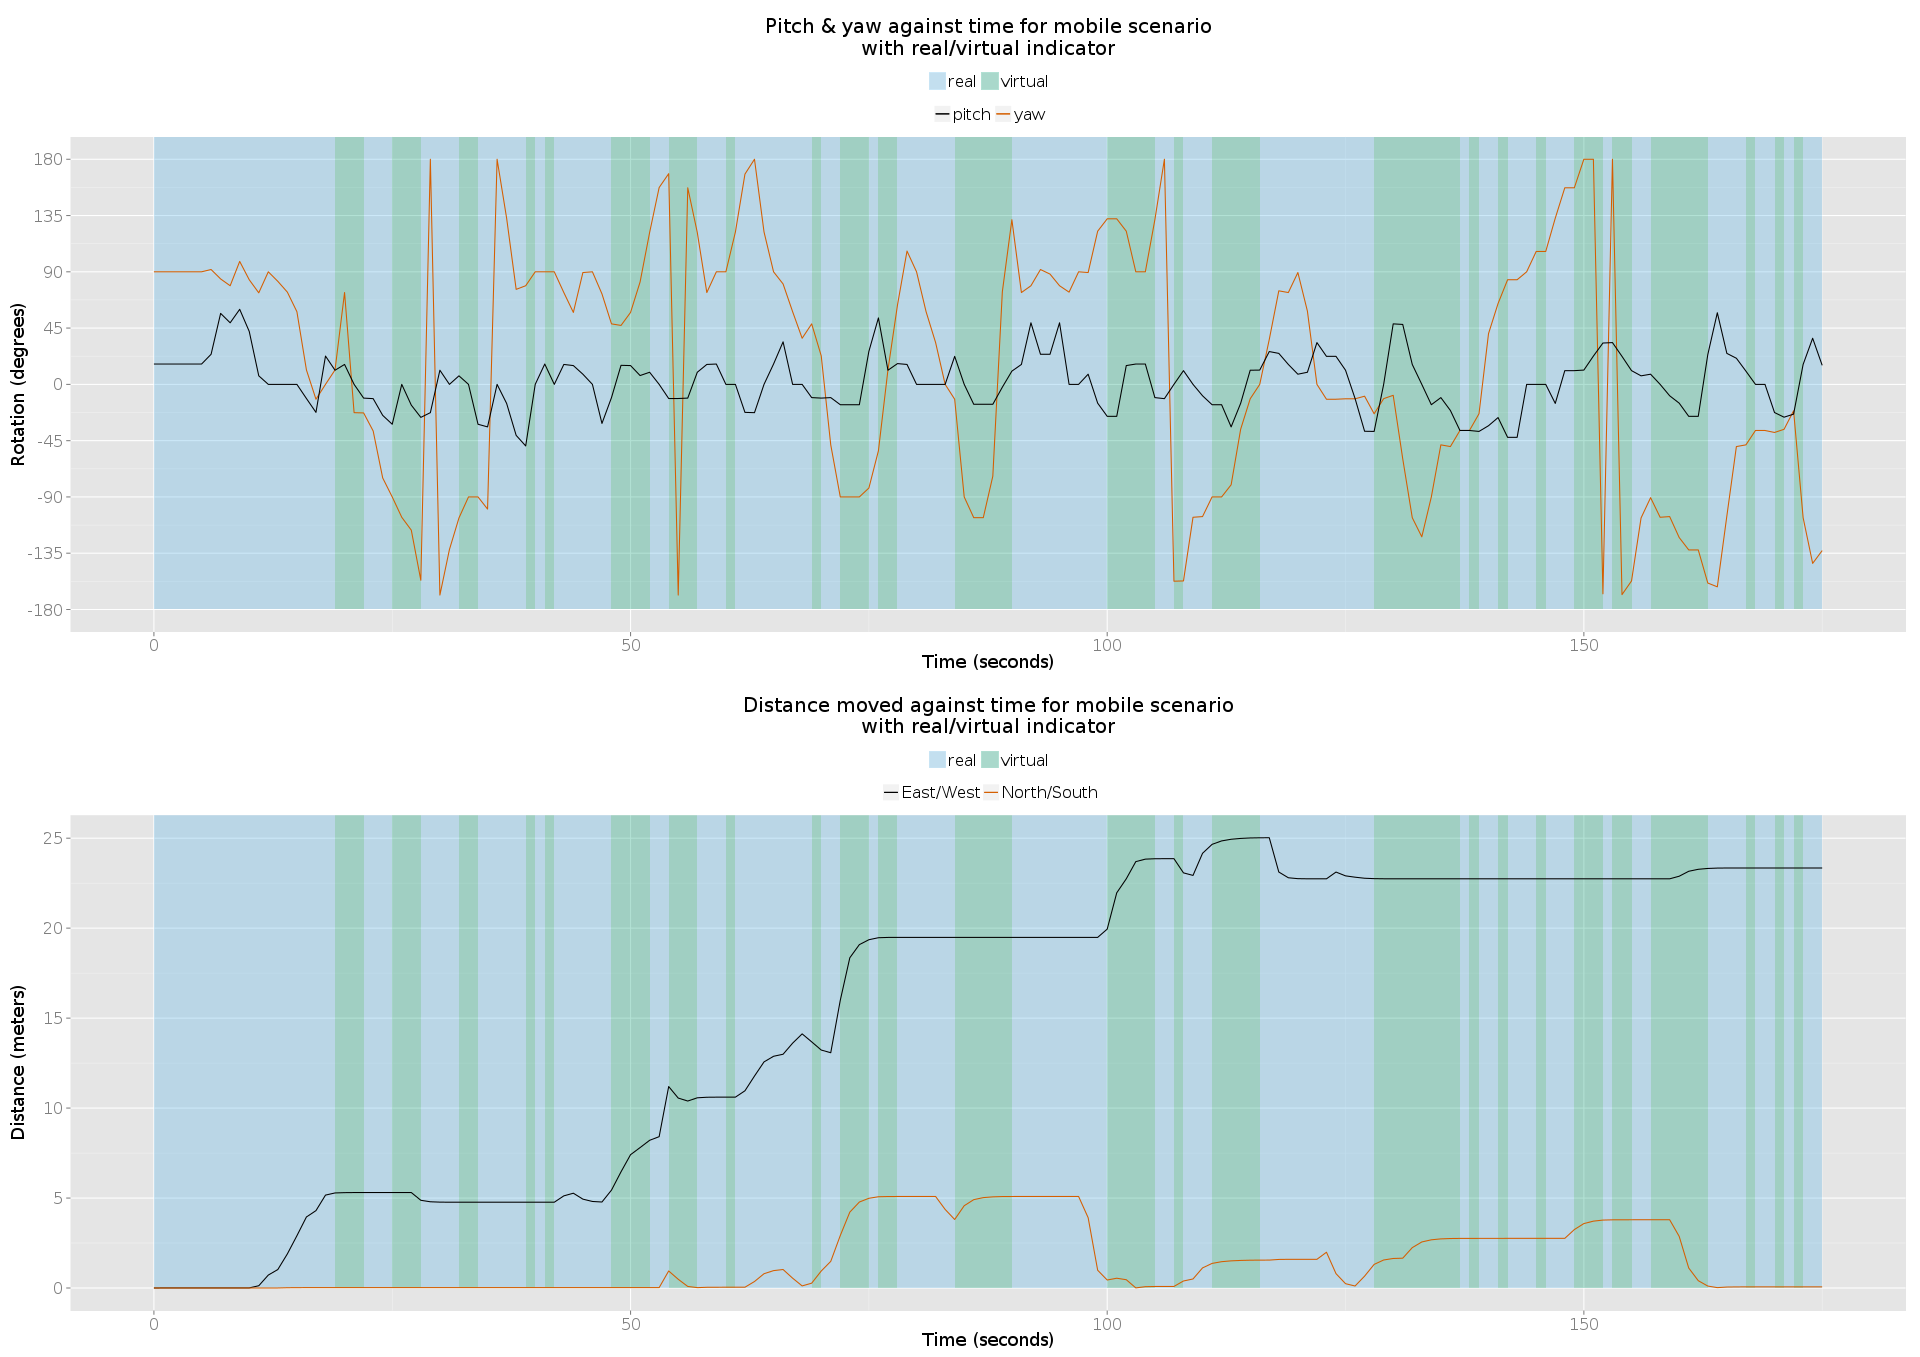
\includegraphics[width=\textwidth]{1/6_2up.png}
	\caption{Some images, yah.}
	\end{center}
\end{figure}

%=========================================================================================================





















%=========================================================================================================
%=========================================================================================================
%=========================================================================================================
%=========================================================================================================
%=========================================================================================================
%=========================================================================================================
%=========================================================================================================

\clearpage

\section{Stage 2}

\begin{figure}[h]
	\begin{center}
		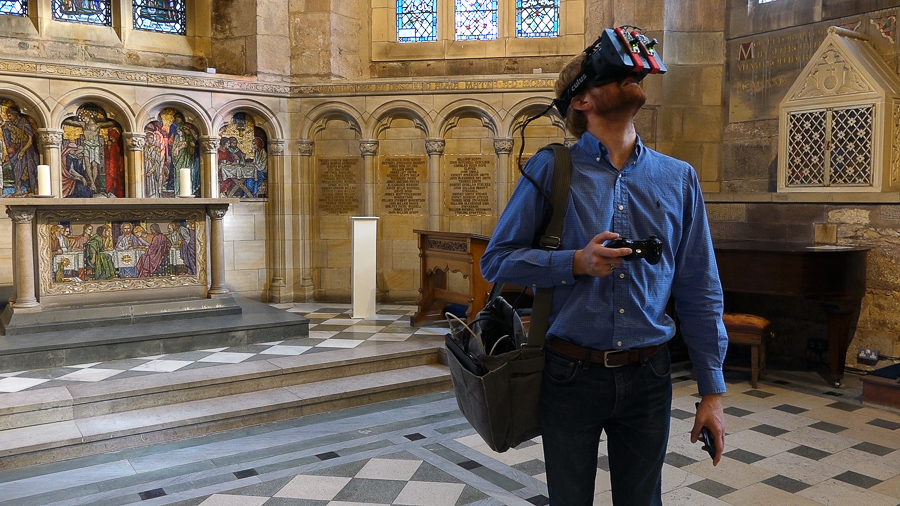
\includegraphics[width=\linewidth]{participant-m.png}
		\caption{participant-m.png}
		\label{participant-m.png}
	\end{center}
\end{figure}

\subsection{Evaluation}

Evaluating users' preferences toward different methods of transitioning between visual stimuli in different situations pertains to studying their reactions \& responses to ascertain the effect upon their focus of attention, concepts which are largely psychological in nature \& highly subjective~\cite{Ijsselsteijn2001}. Thus, subjective measures will produce the bulk of the data for evaluation. However, objective data will also be collected \& cross referenced with the subjective data in attempts to support or contradict any relationships that are identified.

It is hypothesized that a manner of transitioning between visual stimuli which results in a less severe BIP will be preferable to a manner of transitioning which results in a worse BIP. As focus in the Waterworth model is most closely related to presence in the VR literature~\cite{Waterworth2001}, one of the subjective measures that will be used in this evaluation will be an established presence measure, to try to capture the behaviour of the user's position upon the focus axis.

\subsubsection{Subjective Quantitative - Post-Task Questionnaire}
After completing the task, participants will respond to the Igroup Presence Questionnaire (IPQ)~\cite{Schubert2001} (see appendix \ref{ipqitems} for the items of the IPQ) which will provide subjective quantitative insight into their experiences with the system, in particular in relation to their position upon the focus axis of the combined model. The IPQ represents a useful questionnaire for evaluation of users' subjective experiences of using the Mirrorshades platform because its terms, especially in the `spatial involvement' scale, question about the RW environment in a manner that does not explicitly present it as a `distraction' from the VR interaction as many other presence questionnaires do.
%examples of other presence questionnaires that present RW stimuli as 'distractions'?

%citation for the components being independent
%The IPQ consists of one general item (G), five items in the `spatial presence' (SP) scale, four items in the `involvement' scale (INV) \& four items in the `realness' scale (REAL). For the purposes of this study, all of the REAL items save REAL2 will be omitted from the questionnaire. The REAL items are primarily concerned with eliciting how `real' participants considered the virtual environment to be. These questions are useful for traditional VR experiences where the user is encouraged to suspend belief \& believe the VR environment they are perceiving to be `real' (the same experiences for which RW stimuli are usually considered a `distraction'). The Mirrorshades platform, however, is less concerned with convincing participants that a VR environment is real \& is more concerned with the juxtaposition of VR \& RW environments.
%It is believed that the other REAL questions will get the participants thinking about the wrong things & hamper their responses when talking about XR

%hypothesis
Whilst a traditional VR experience would hope to elicit high SP1 \& SP4 results combined with low INV1 \& INV3 results, Mirrorshades participants are expected to report high SP1 \& SP4 combined with \textit{high} INV1 \& INV3. The results from participants in this investigation will be compared against those who partook in a `traditional' VR experience wherein RW stimuli were considered a distraction.







These data are expected to reveal relationships between various different metrics \& the choice of transition methods. For example, it is expected that participants will perform short transitions to VR or transitions to a mix of RW \& VR when moving \& perform longer transitions to VR when stationary. This kind of relationship will support or contradict the subjective data collected through questionnaire \& interview.

\section{Phase 2.1 Results}

%=========================================================================================================

\clearpage

\subsection{Participant 7}

\begin{figure}[h]
	\begin{center}
	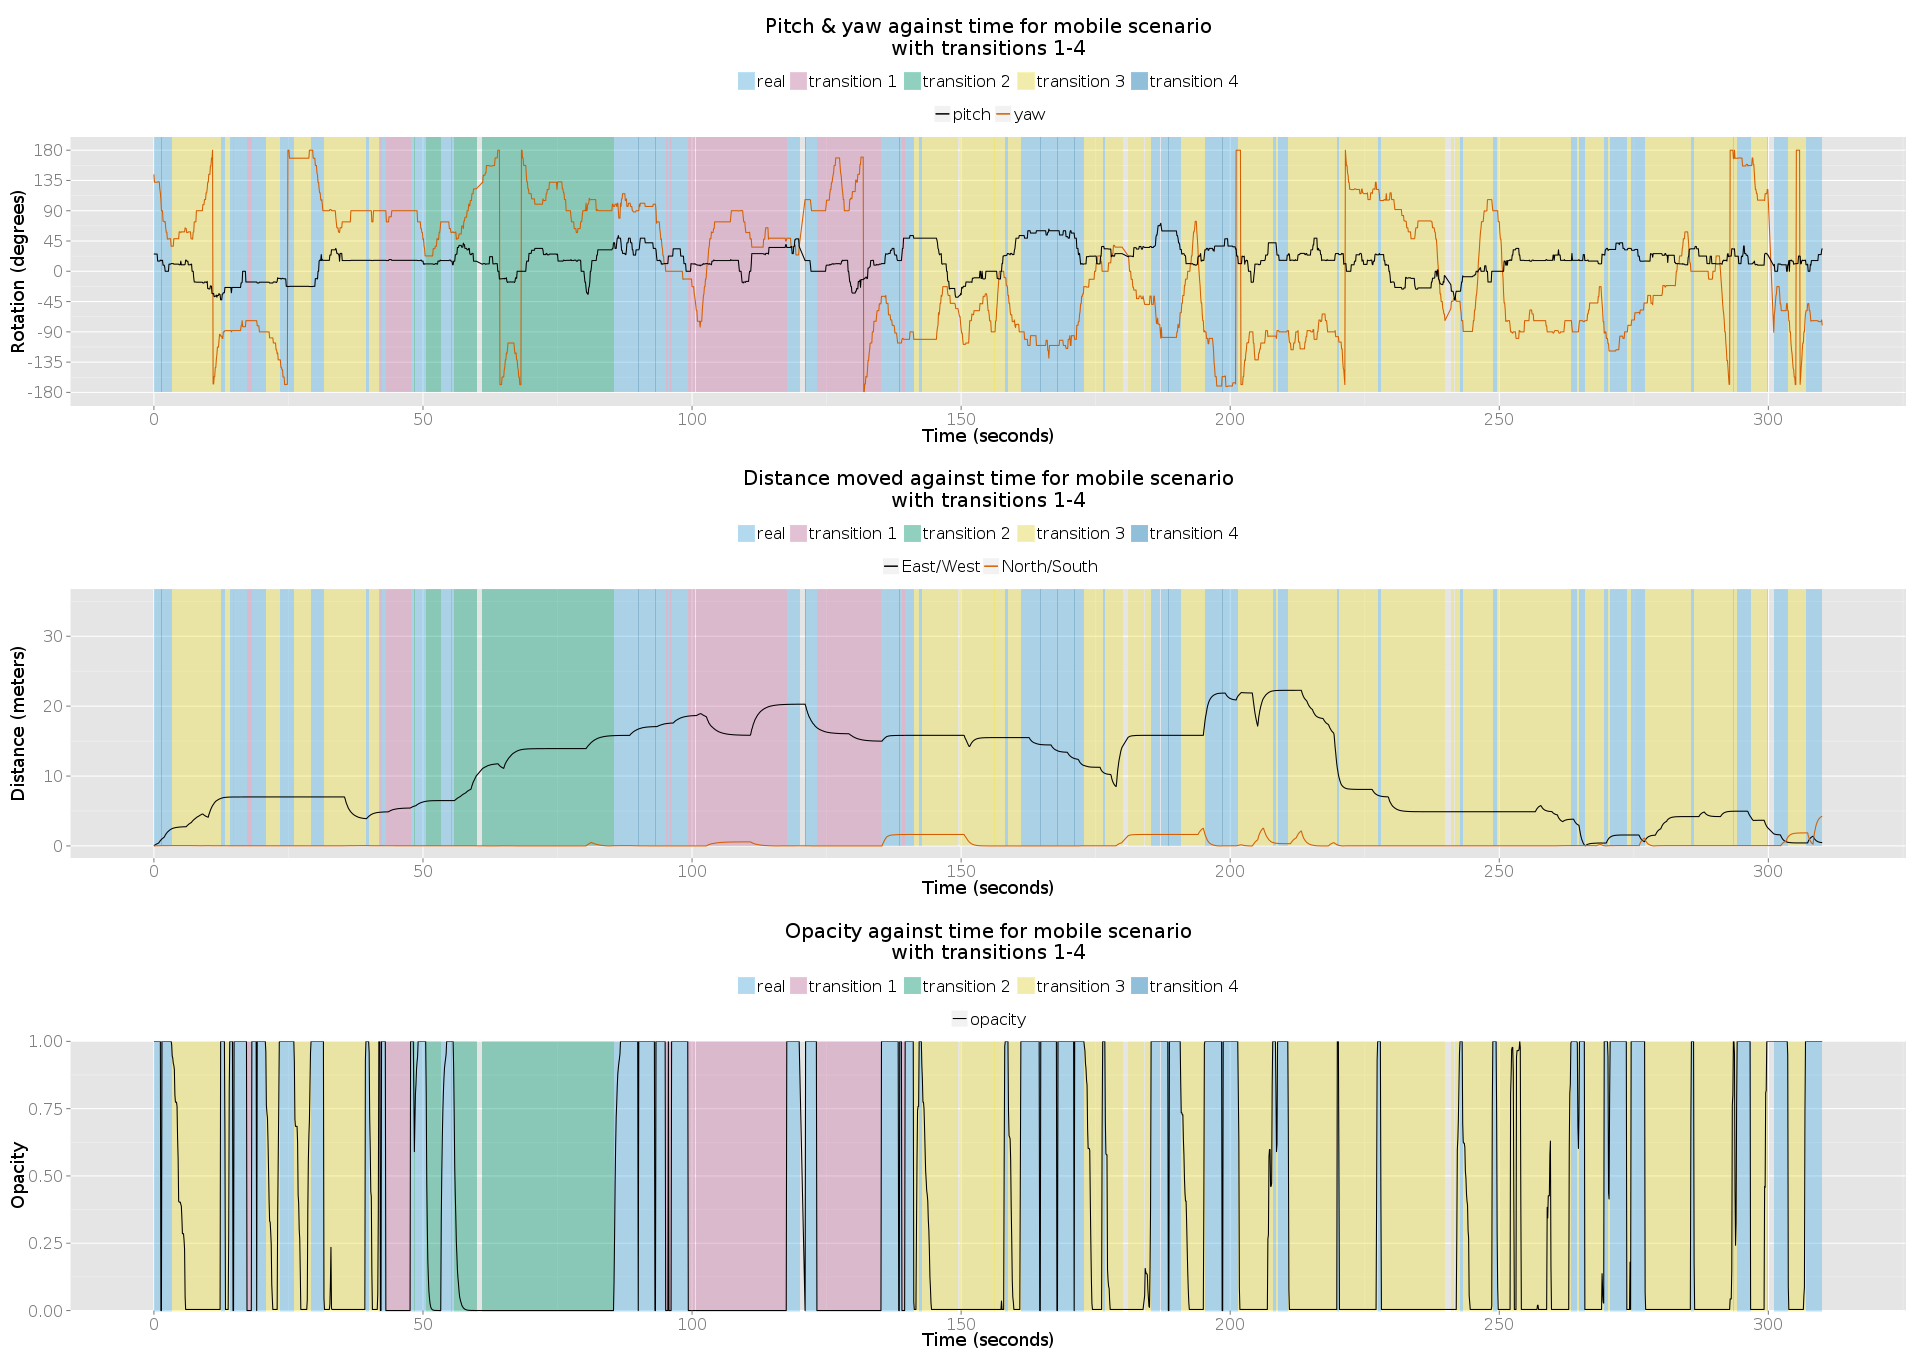
\includegraphics[width=\textwidth]{2.1/7_1-4_3up.png}
	\caption{Some images, yah.}
	\end{center}
\end{figure}

%=========================================================================================================

\clearpage

\subsection{Participant 8}

\begin{figure}[h]
	\begin{center}
	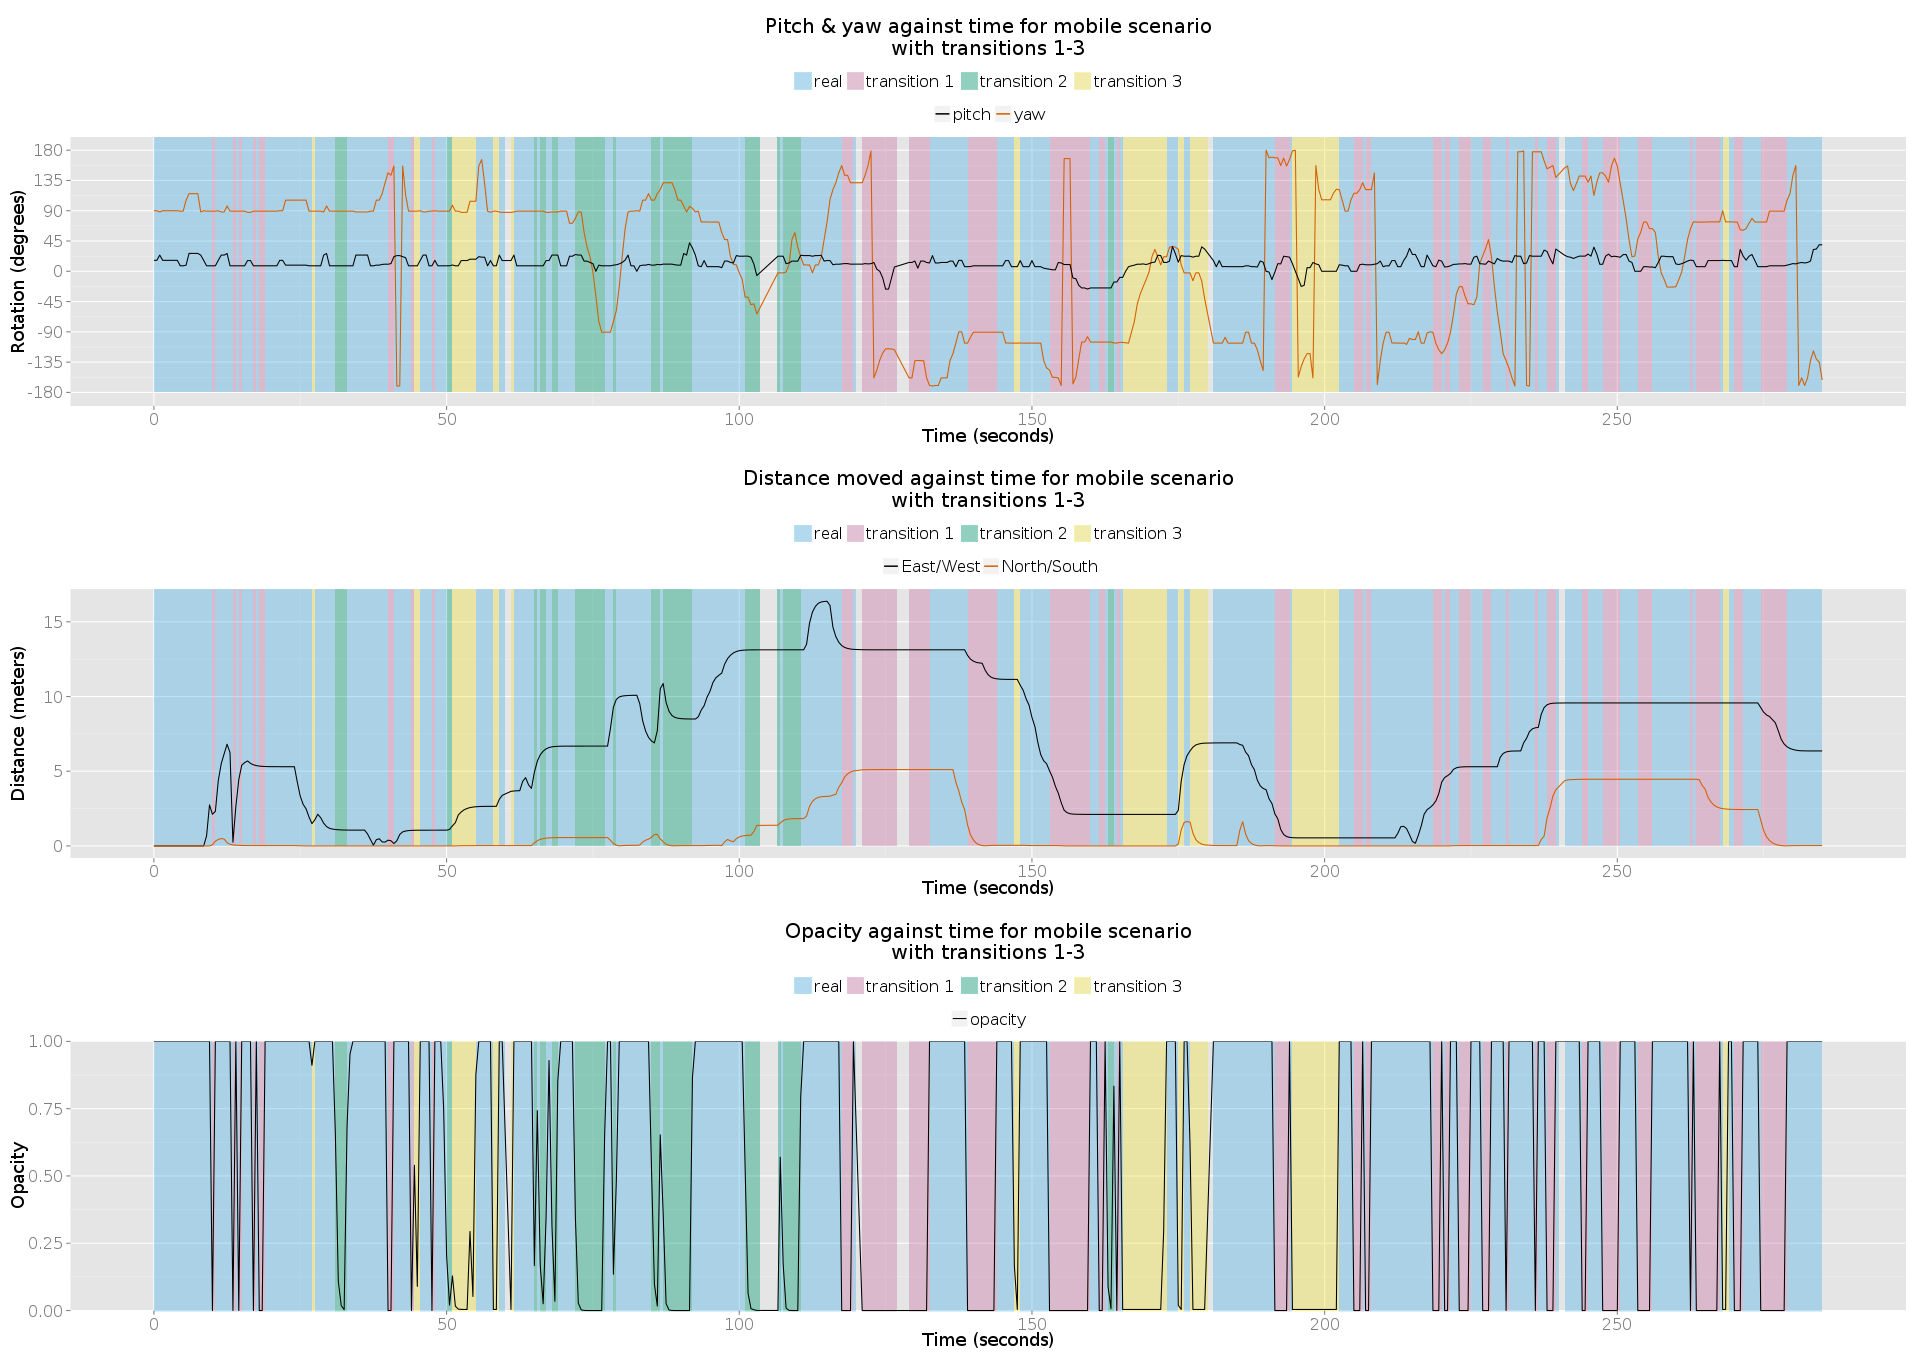
\includegraphics[width=\textwidth]{2.1/8_1-3_3up.png}
	\caption{Some images, yah.}
	\end{center}
\end{figure}

\clearpage

\begin{figure}[h]
	\begin{center}
	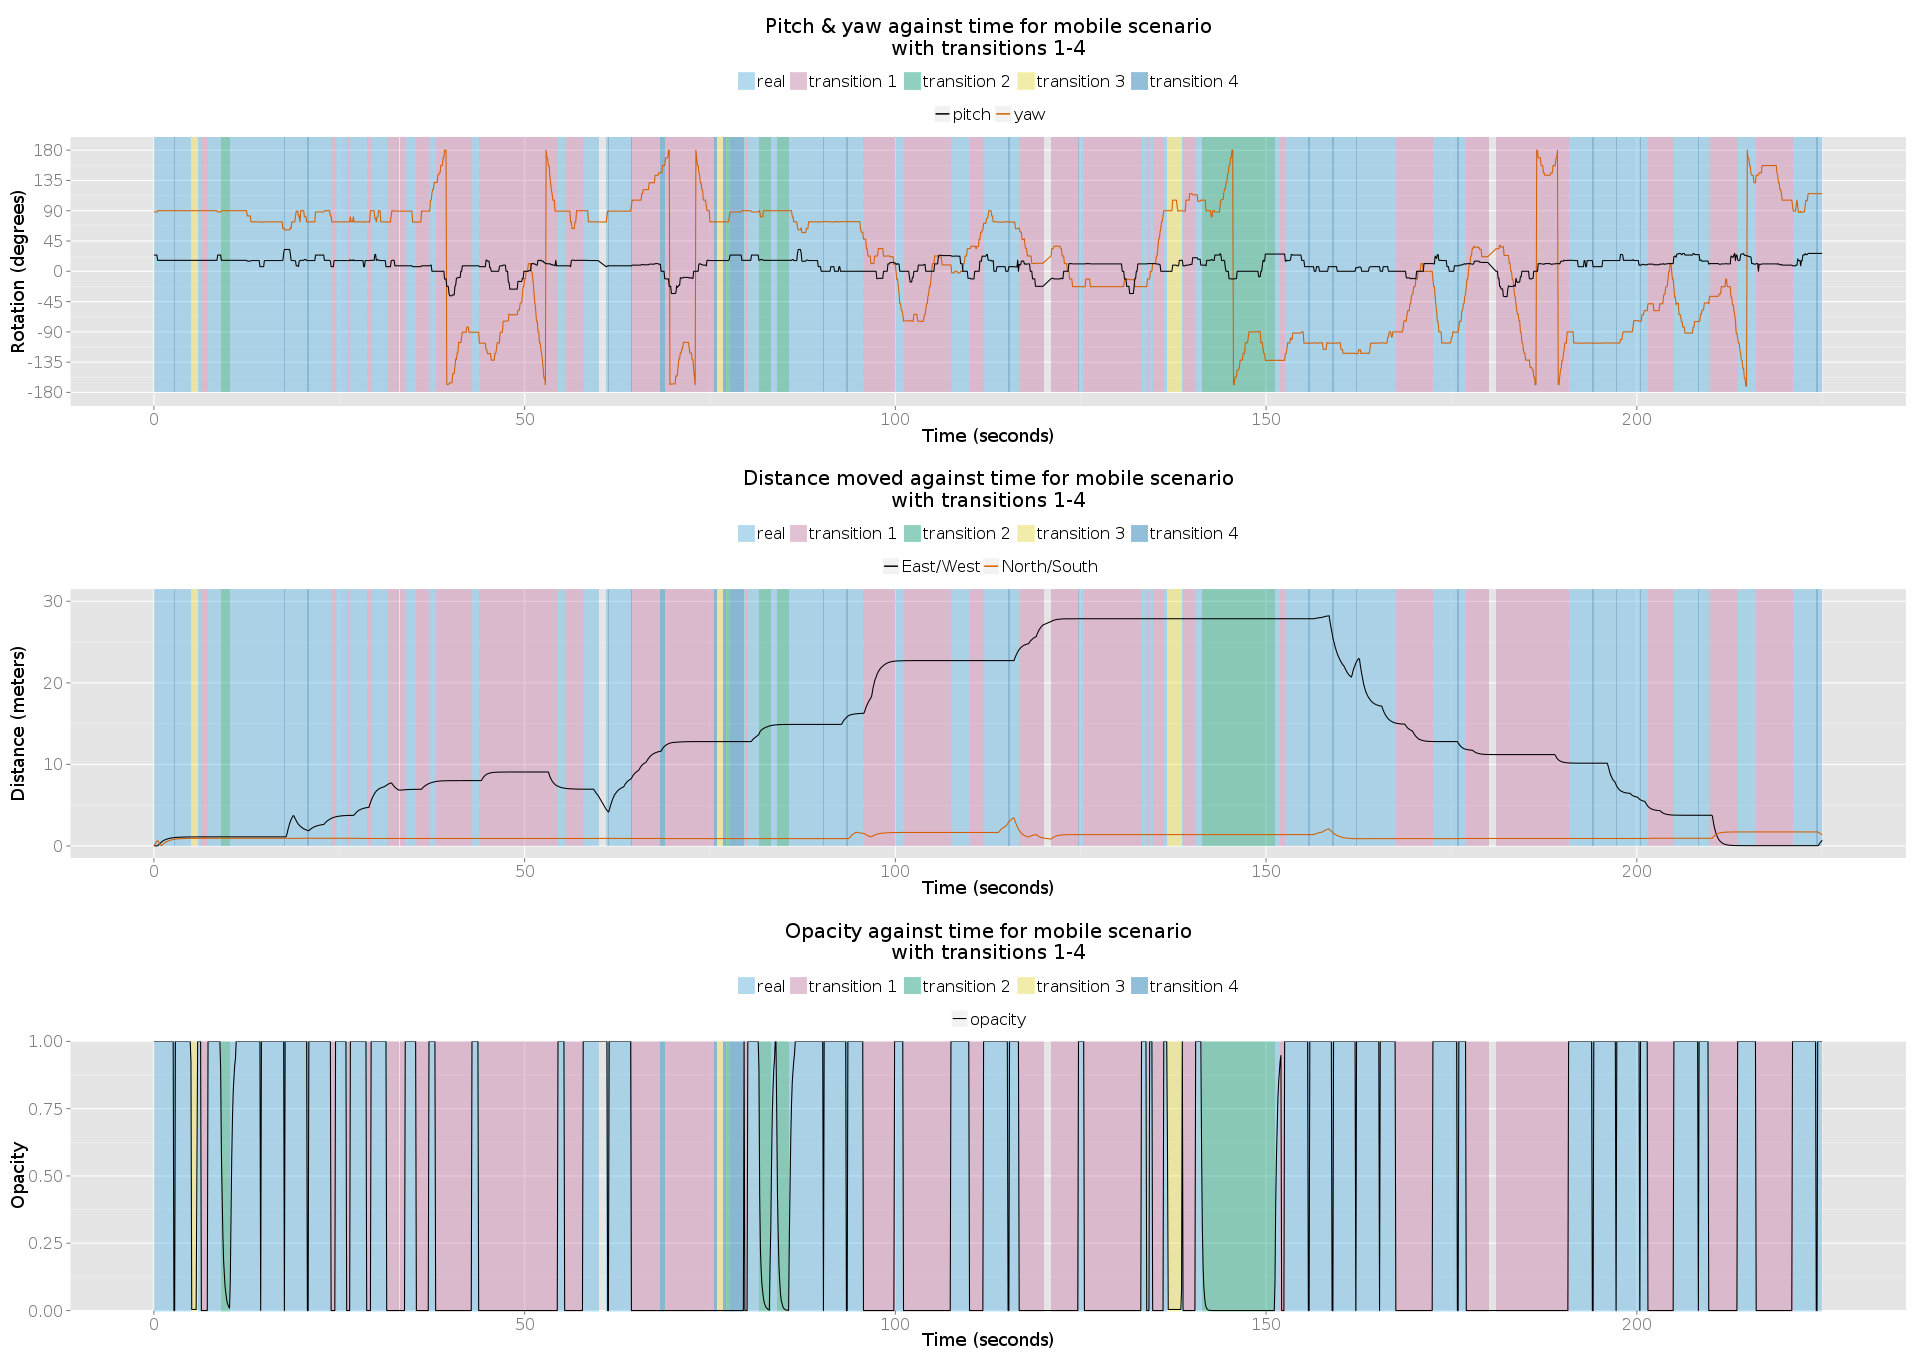
\includegraphics[width=\textwidth]{2.1/8_1-4_3up.png}
	\caption{Some images, yah.}
	\end{center}
\end{figure}

%=========================================================================================================

\clearpage

\subsection{Participant 9}

\begin{figure}[h]
	\begin{center}
	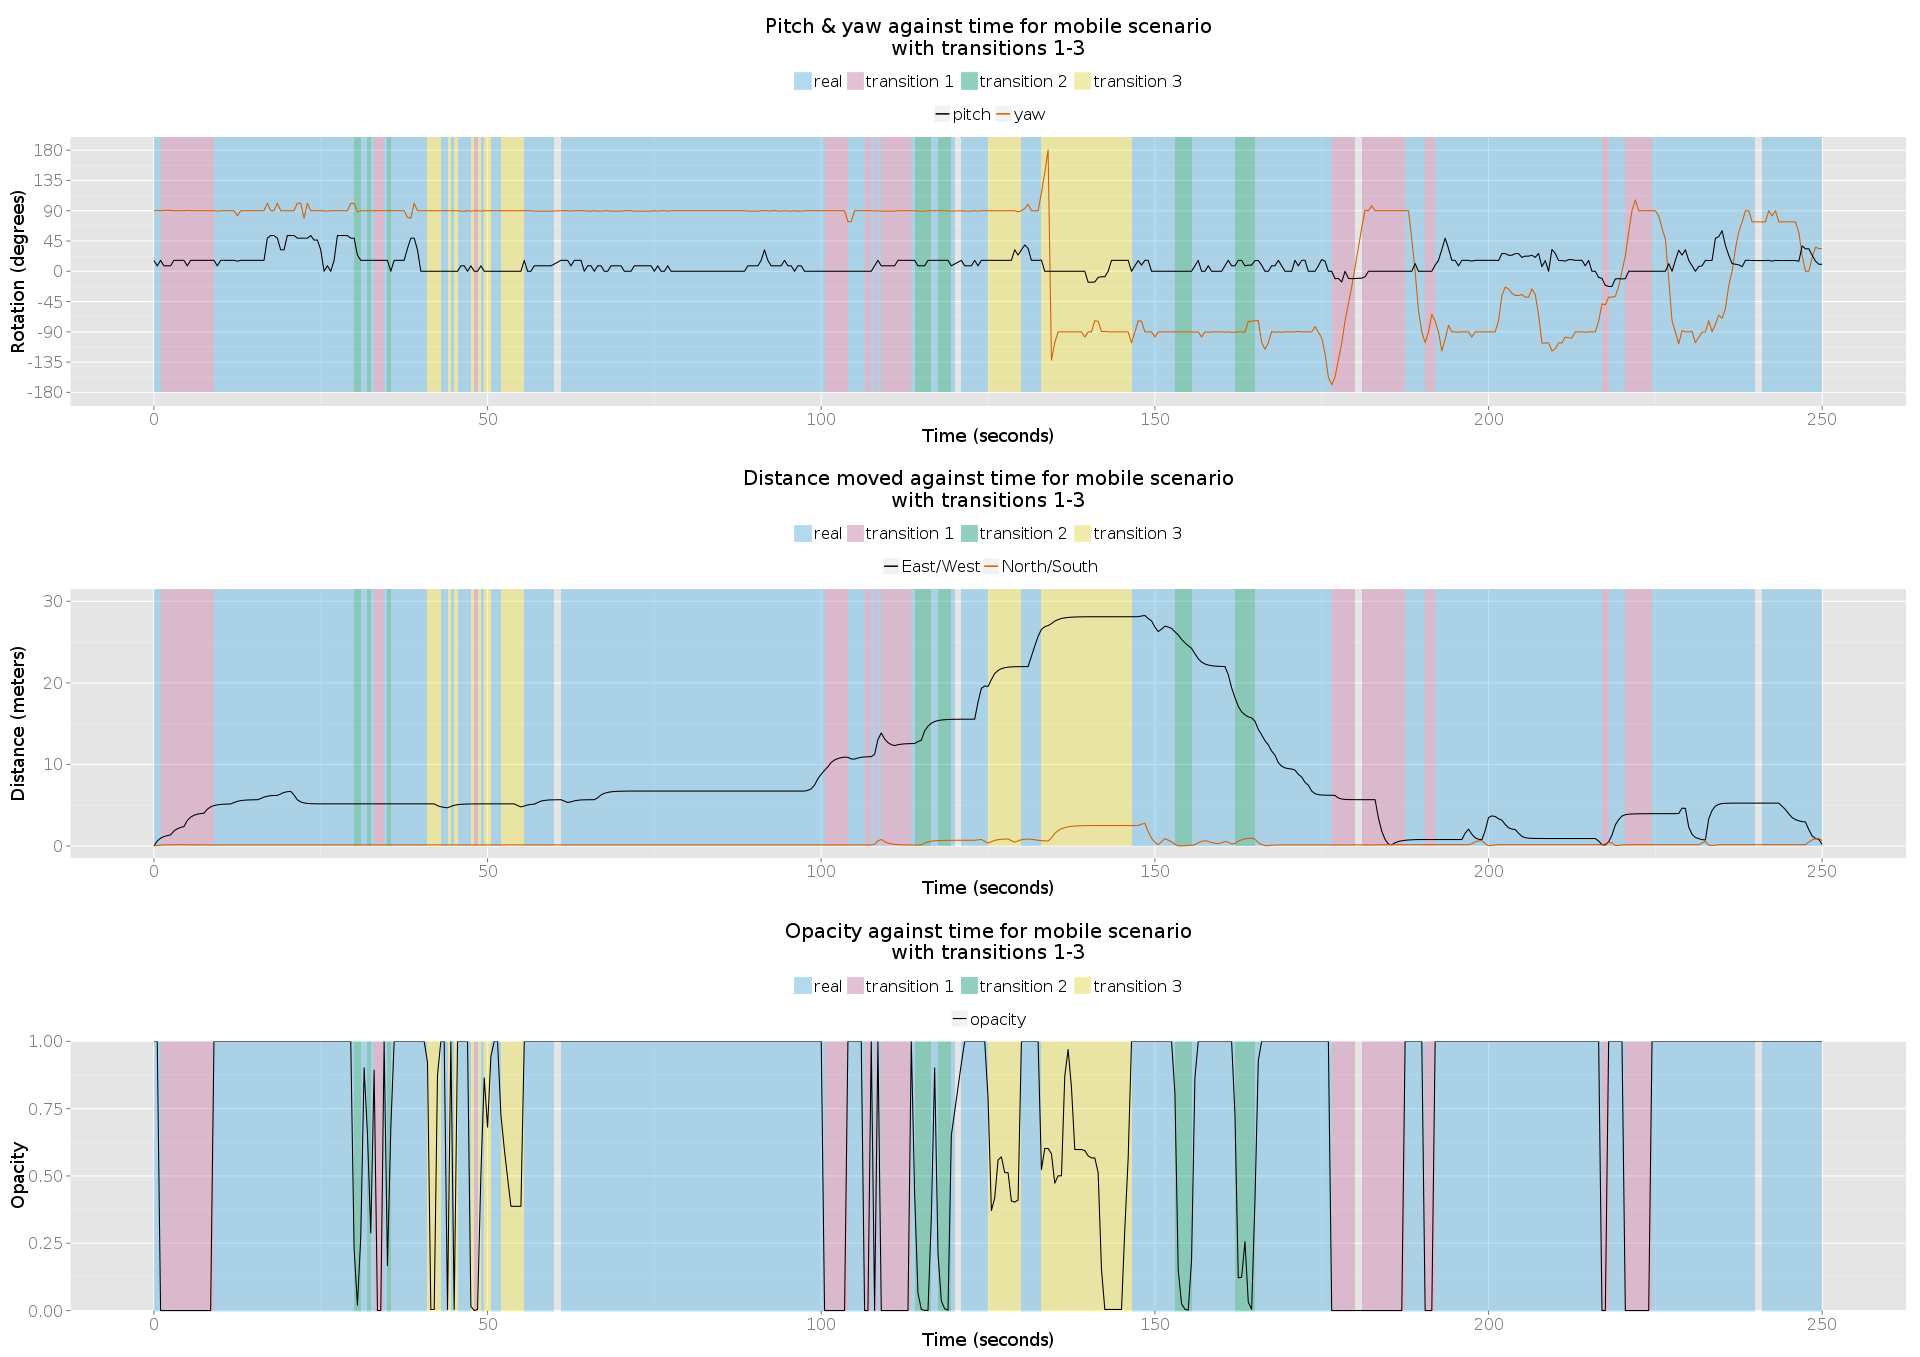
\includegraphics[width=\textwidth]{2.1/9_1-3_3up.png}
	\caption{Some images, yah.}
	\end{center}
\end{figure}

\clearpage

\begin{figure}[h]
	\begin{center}
	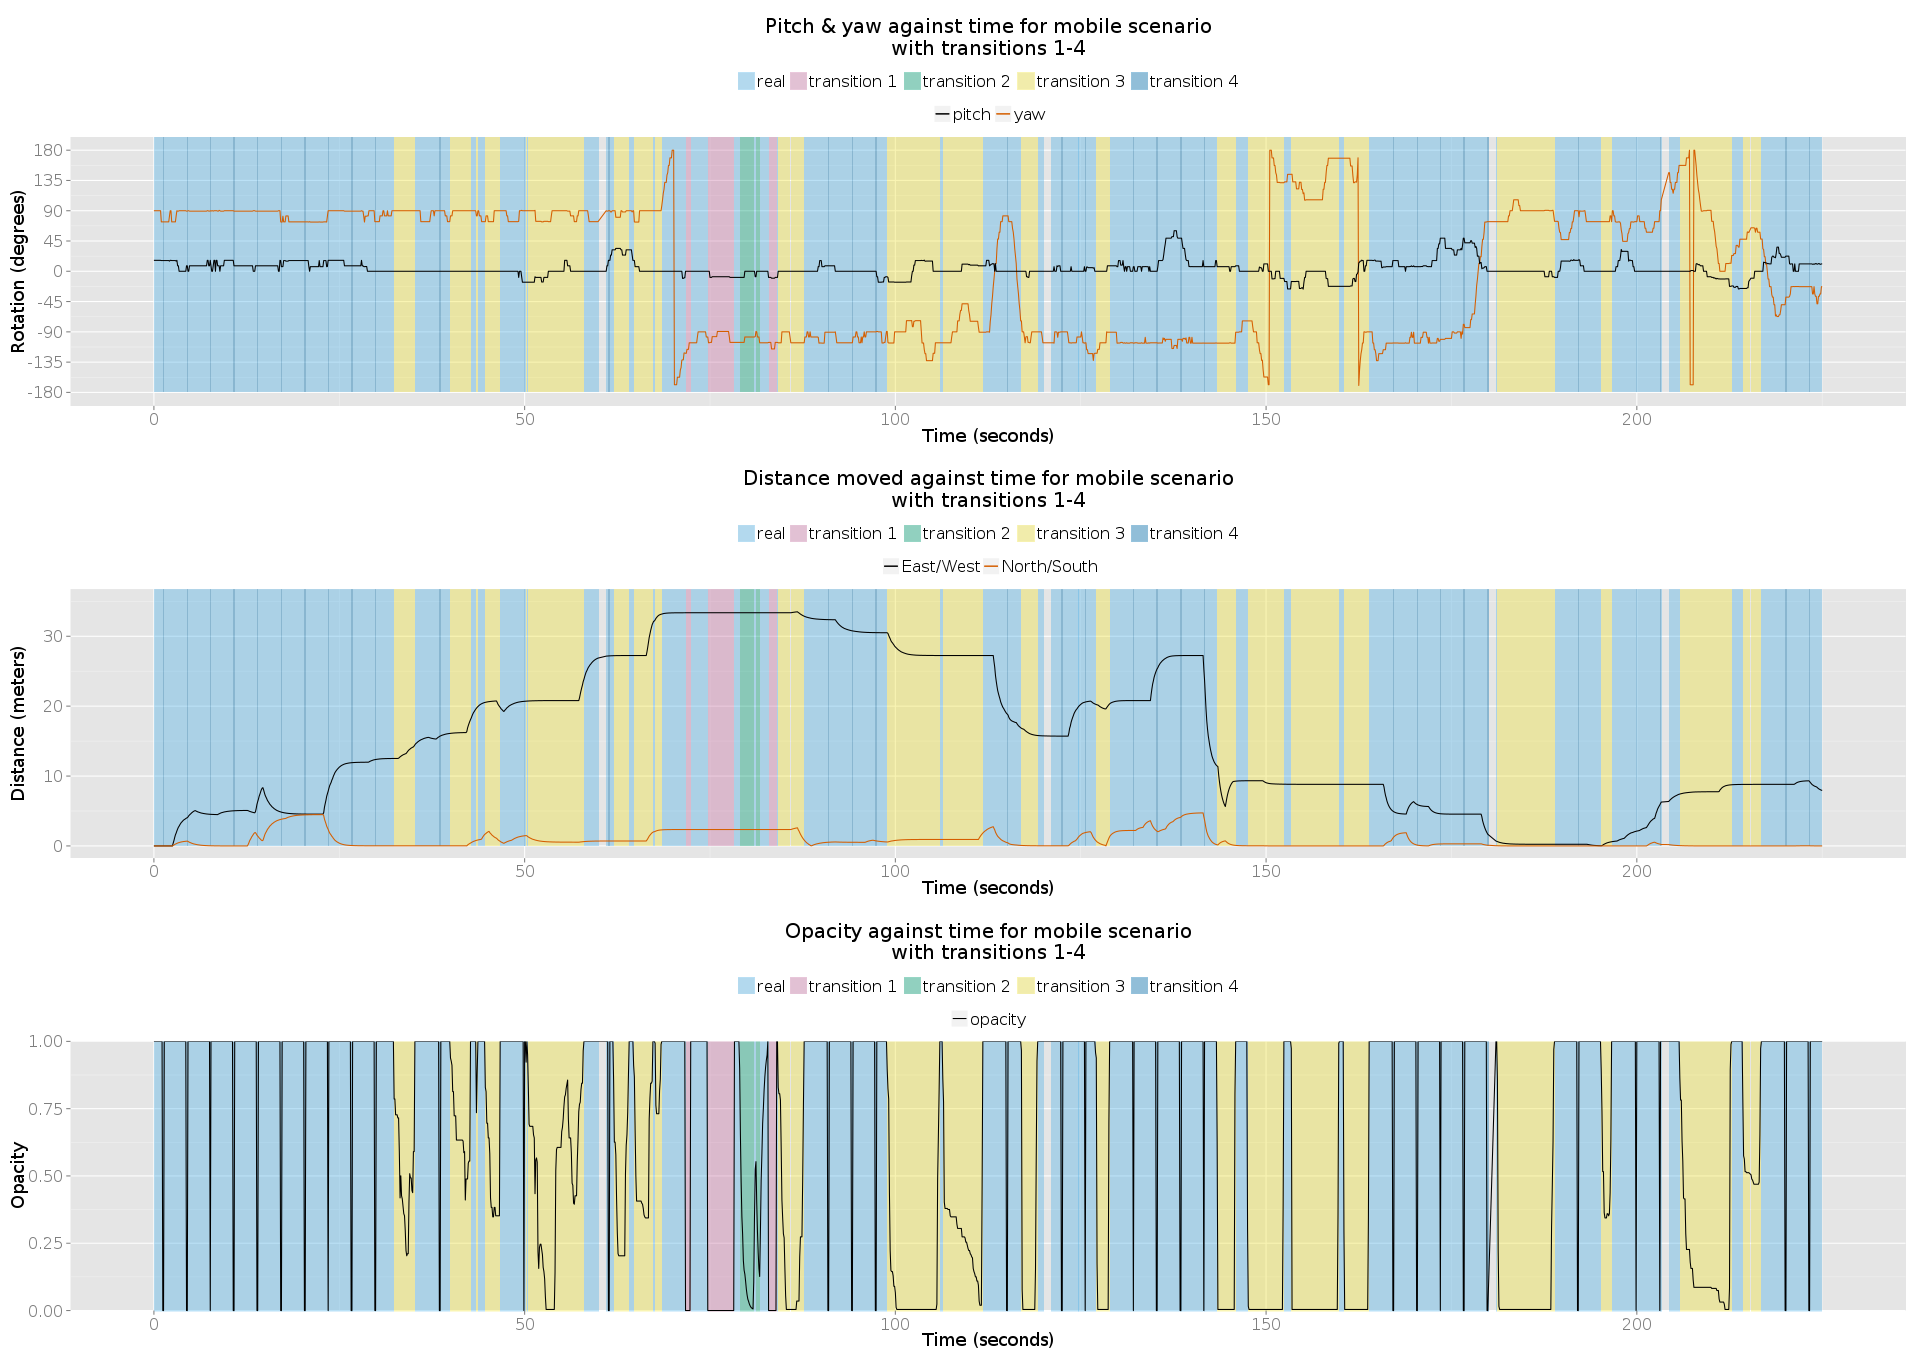
\includegraphics[width=\textwidth]{2.1/9_1-4_3up.png}
	\caption{Some images, yah.}
	\end{center}
\end{figure}

%=========================================================================================================

\clearpage

\subsection{Participant 10}

\begin{figure}[h]
	\begin{center}
	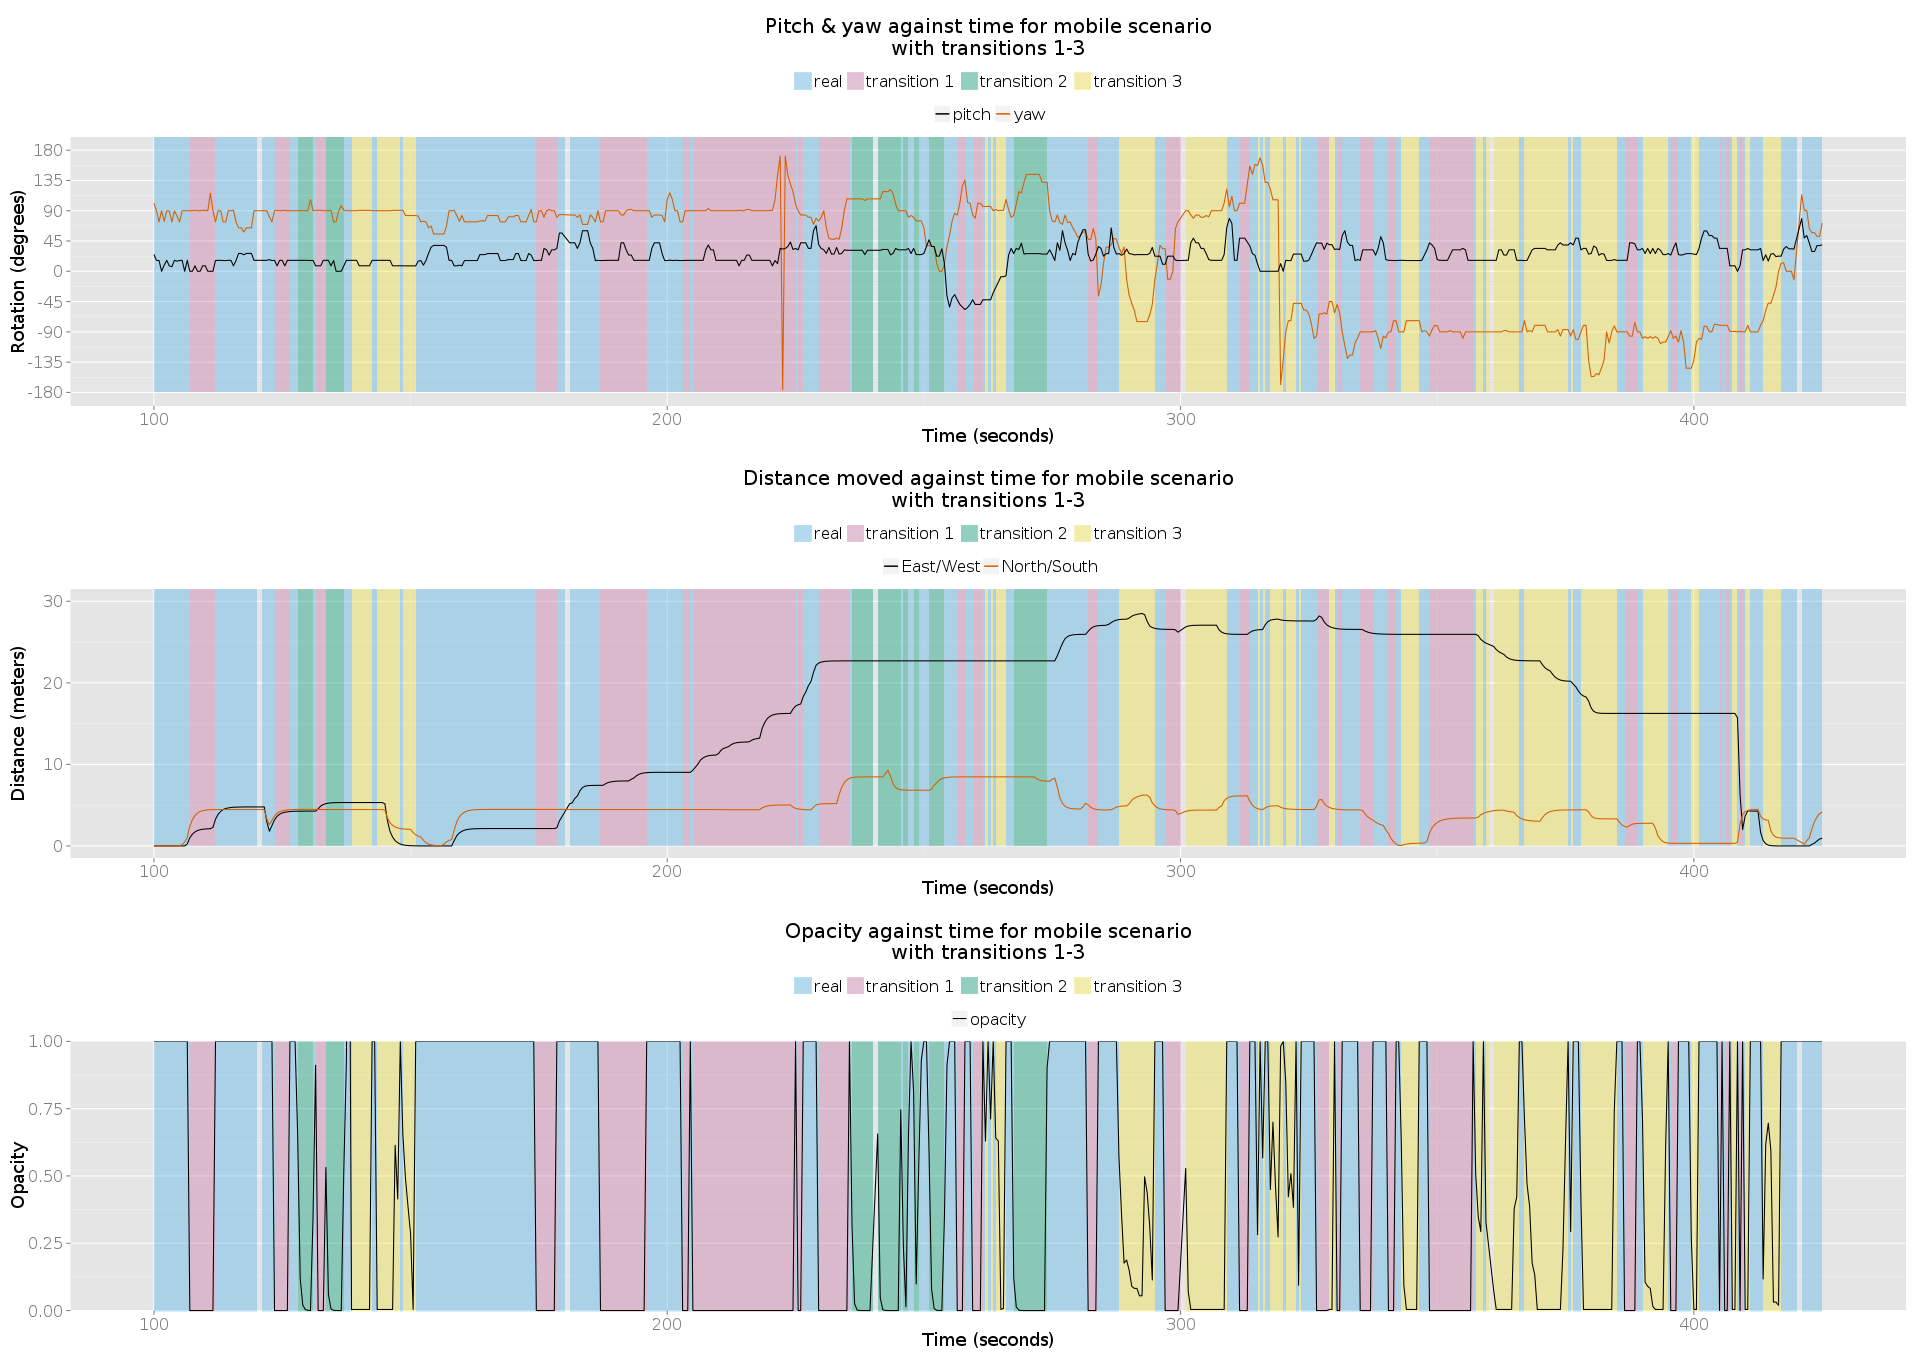
\includegraphics[width=\textwidth]{2.1/10_1-3_3up.png}
	\caption{Some images, yah.}
	\end{center}
\end{figure}

\clearpage

\begin{figure}[h]
	\begin{center}
	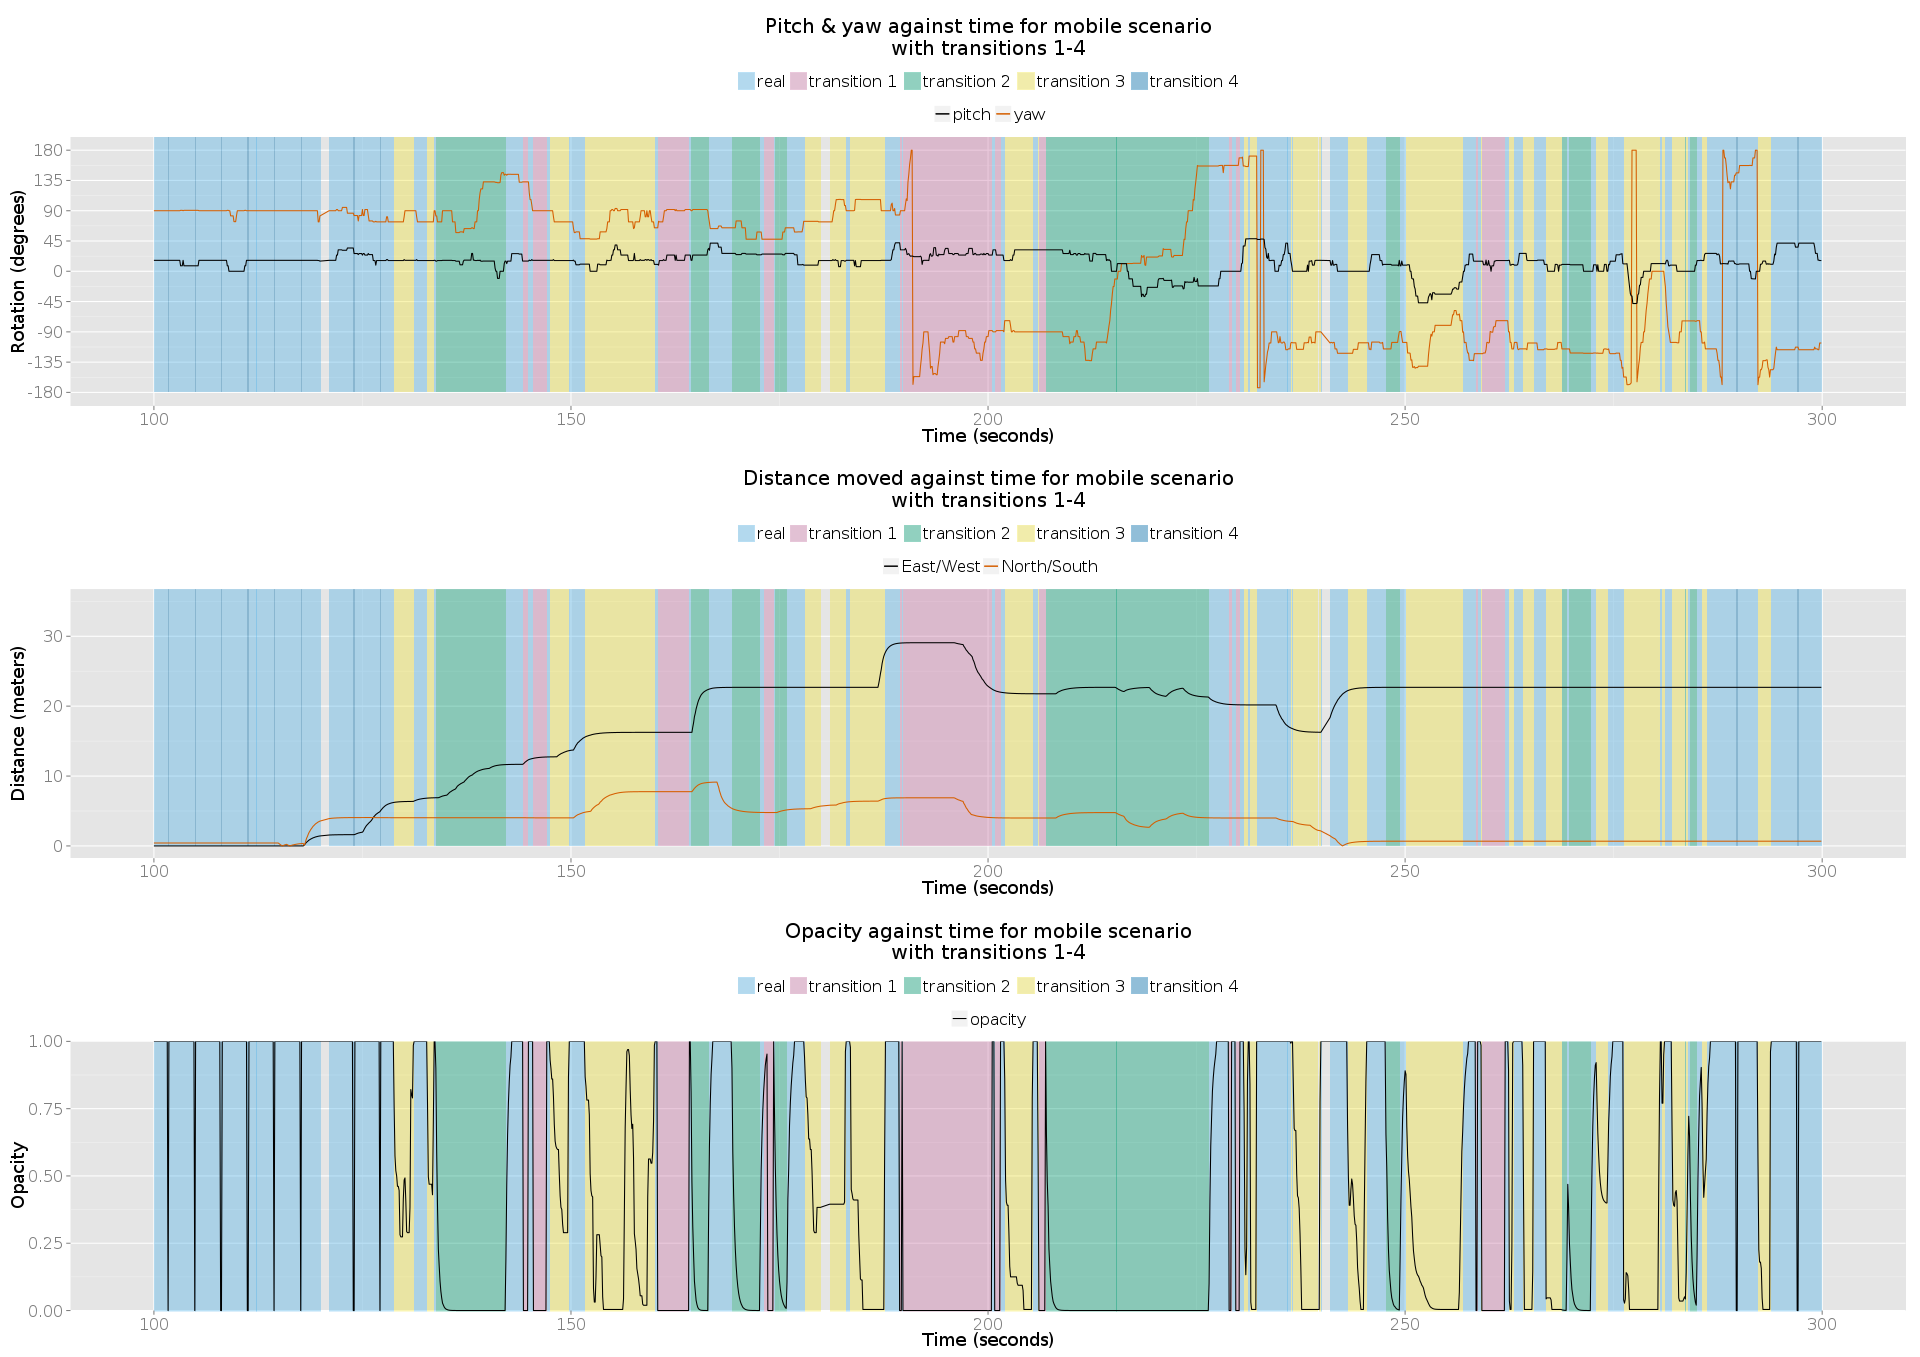
\includegraphics[width=\textwidth]{2.1/10_1-4_3up.png}
	\caption{Some images, yah.}
	\end{center}
\end{figure}

%=========================================================================================================

\clearpage

\subsection{Participant 11}

\begin{figure}[h]
	\begin{center}
	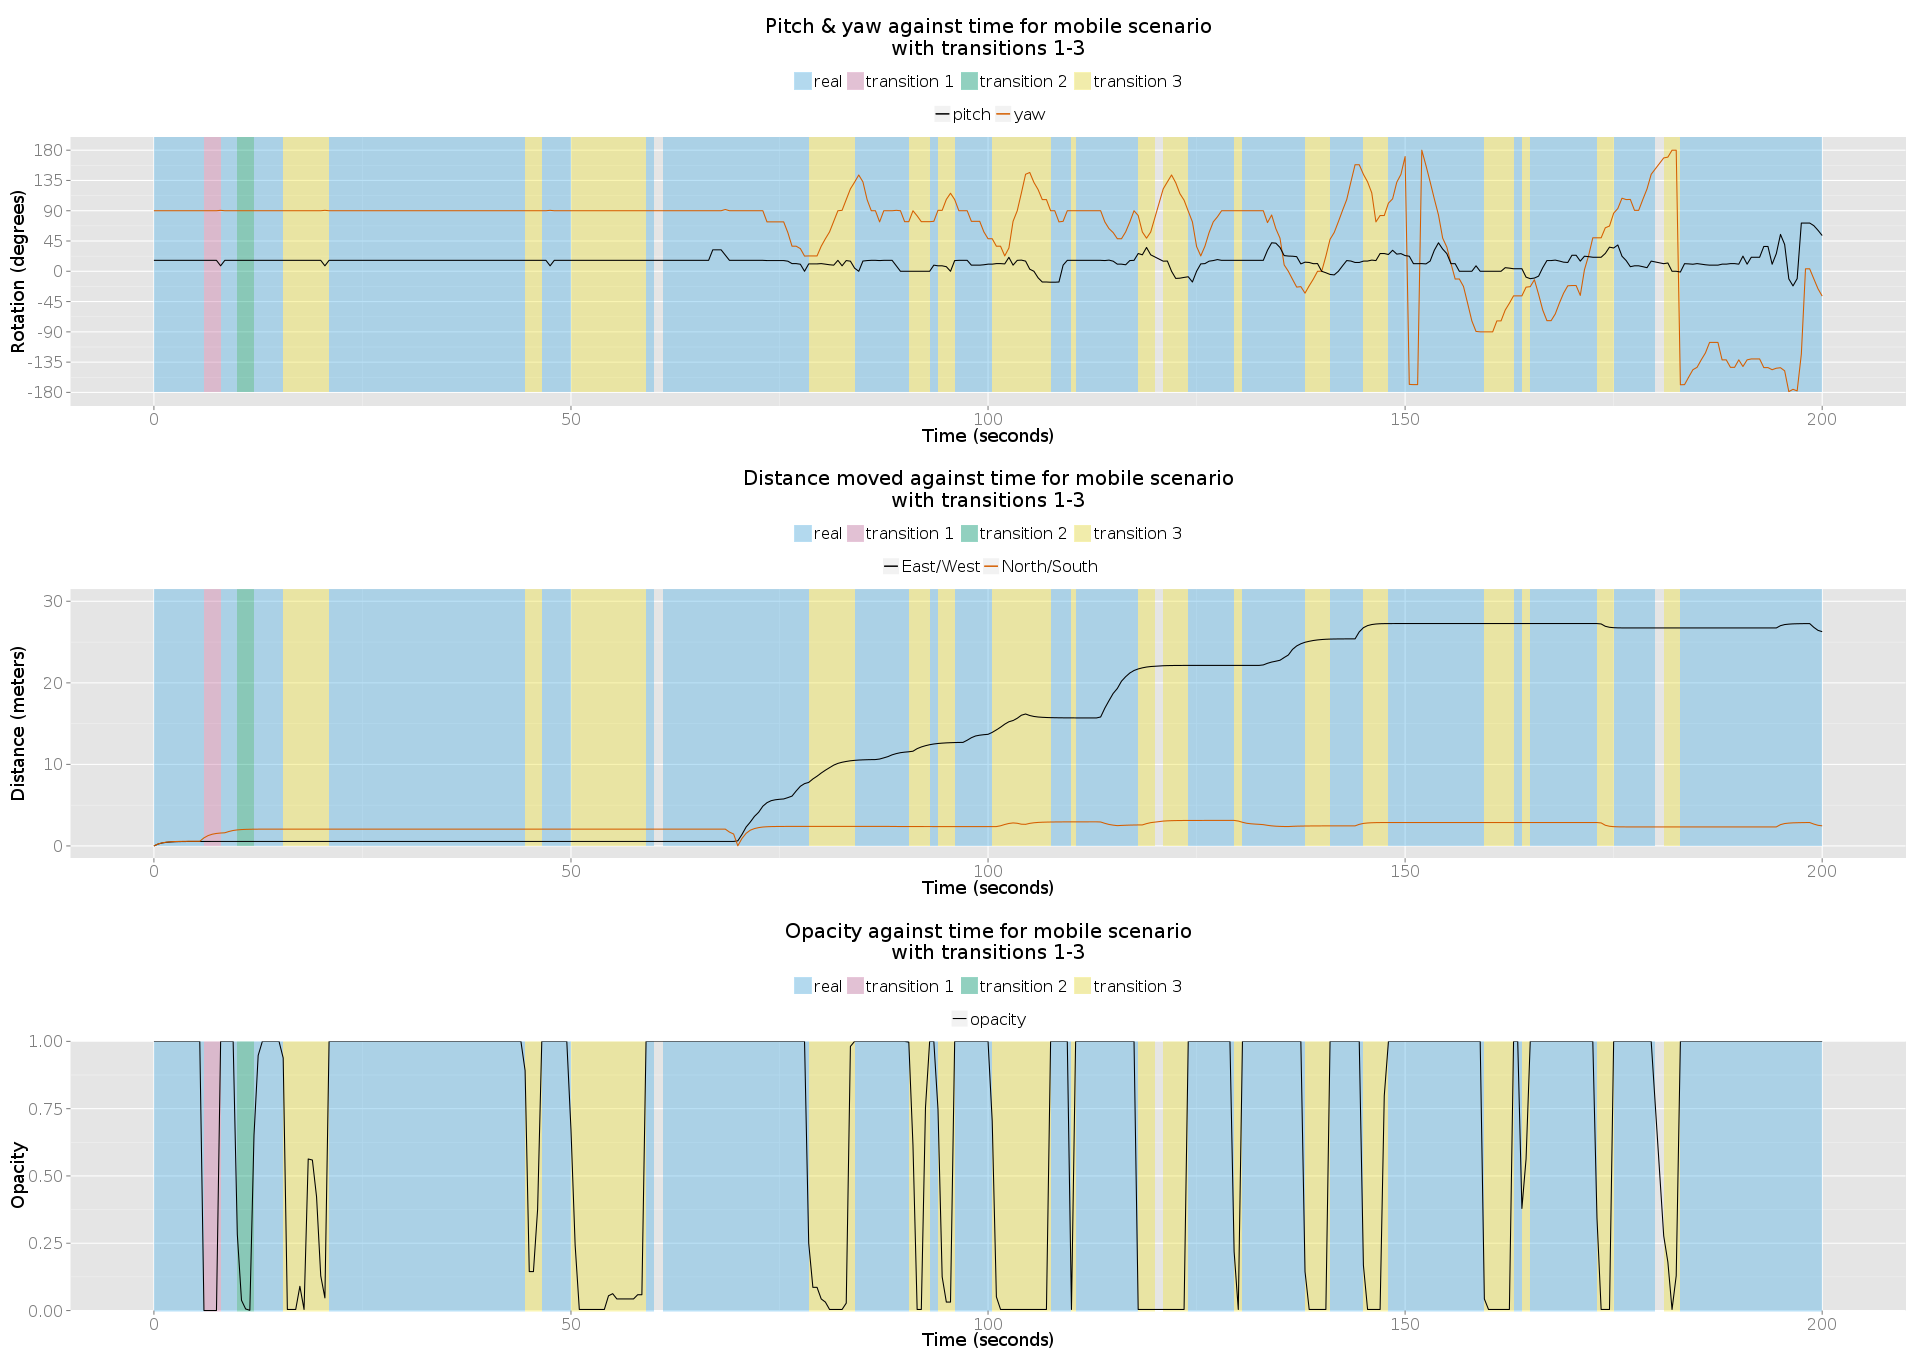
\includegraphics[width=\textwidth]{2.1/11_1-3_3up.png}
	\caption{Some images, yah.}
	\end{center}
\end{figure}

\clearpage

\begin{figure}[h]
	\begin{center}
	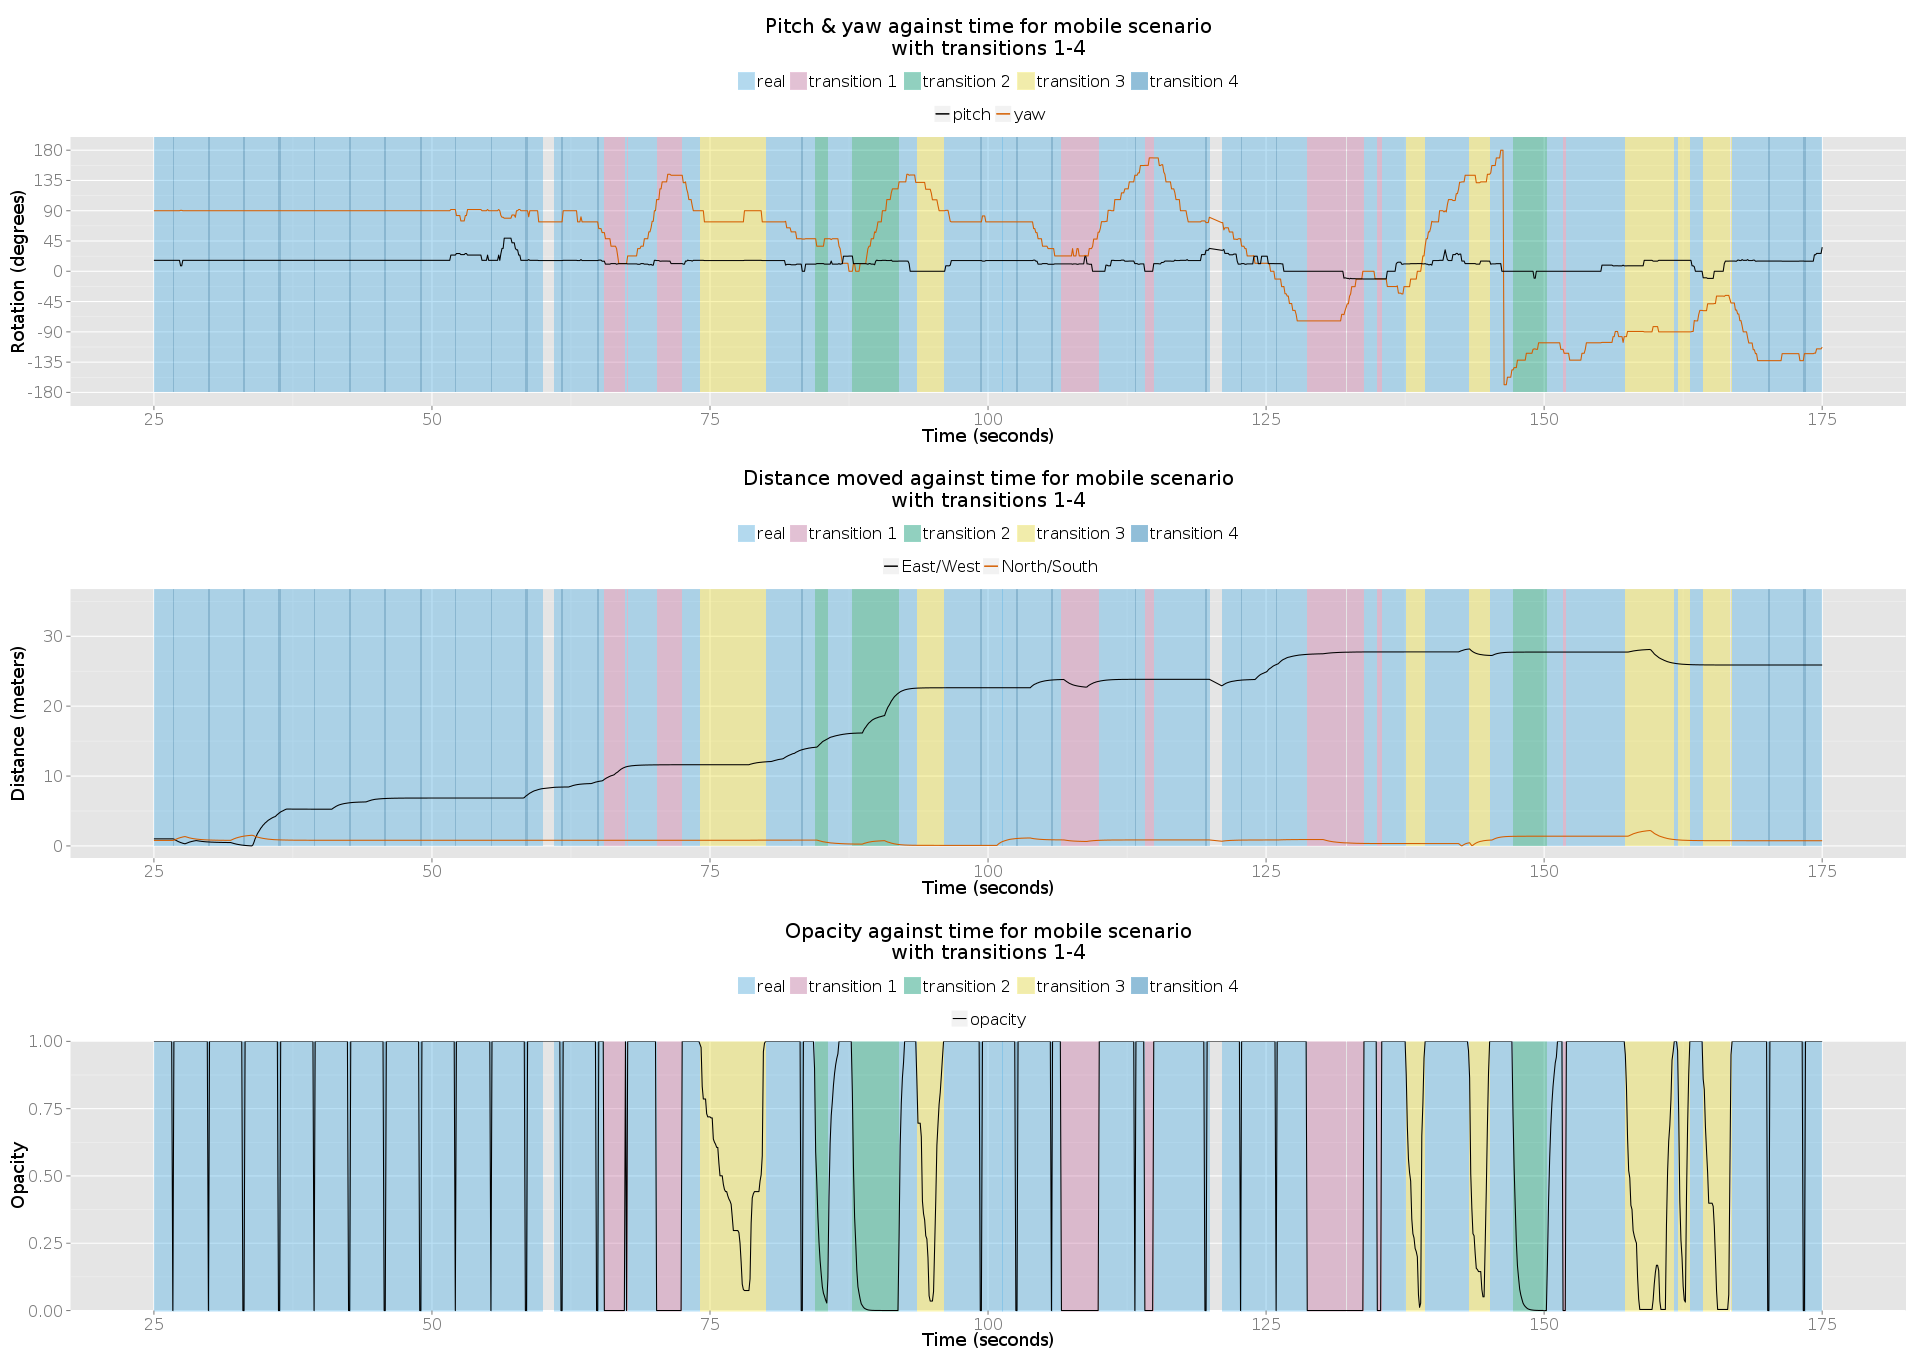
\includegraphics[width=\textwidth]{2.1/11_1-4_3up.png}
	\caption{Some images, yah.}
	\end{center}
\end{figure}

%=========================================================================================================

\clearpage

\subsection{Participant 12}

\begin{figure}[h]
	\begin{center}
	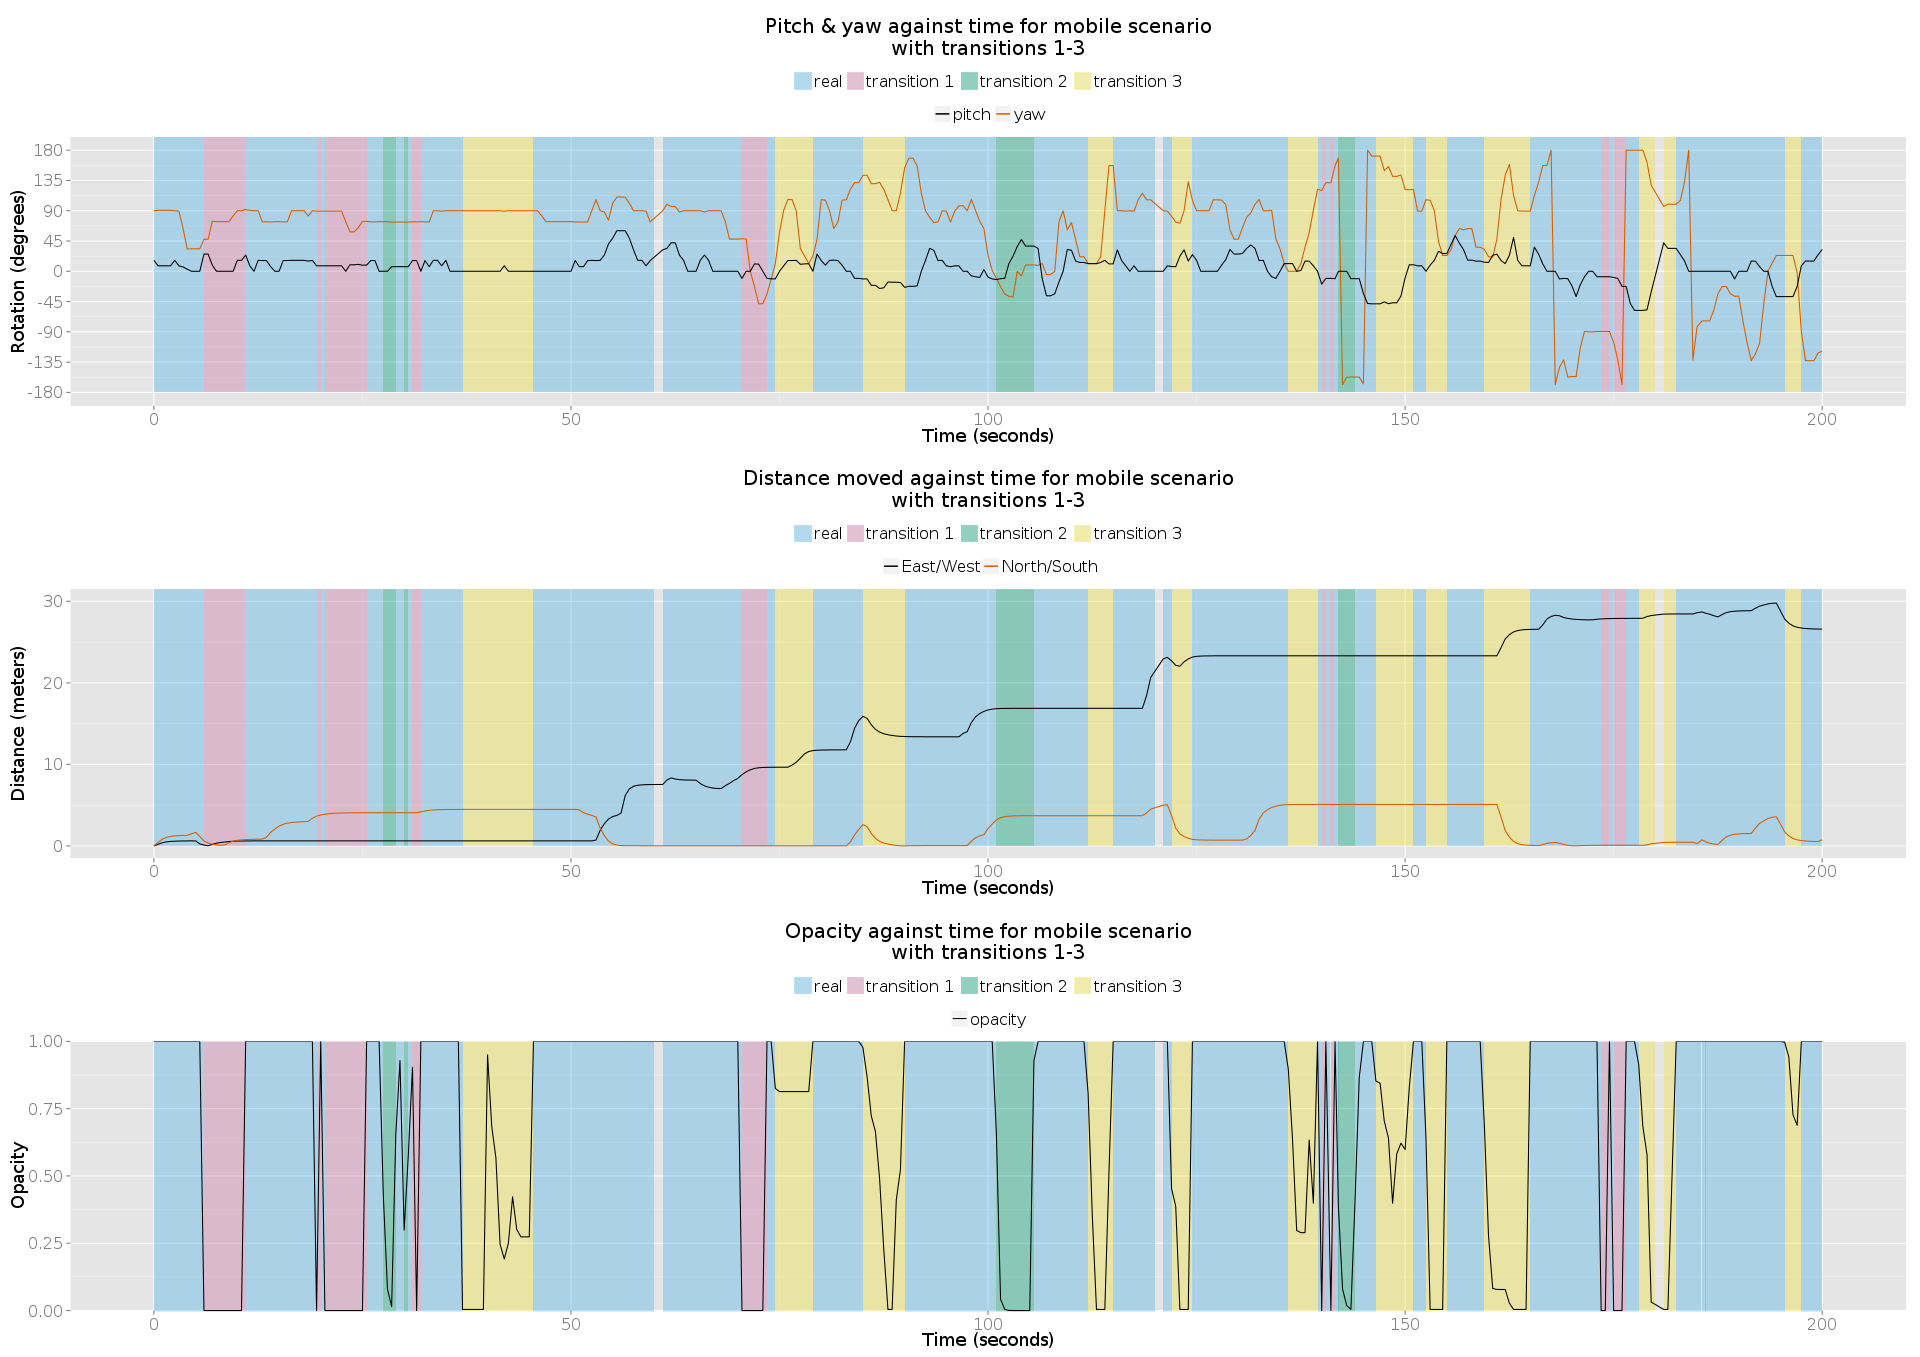
\includegraphics[width=\textwidth]{2.1/12_1-3_3up.png}
	\caption{Some images, yah.}
	\end{center}
\end{figure}

\clearpage

\begin{figure}[h]
	\begin{center}
	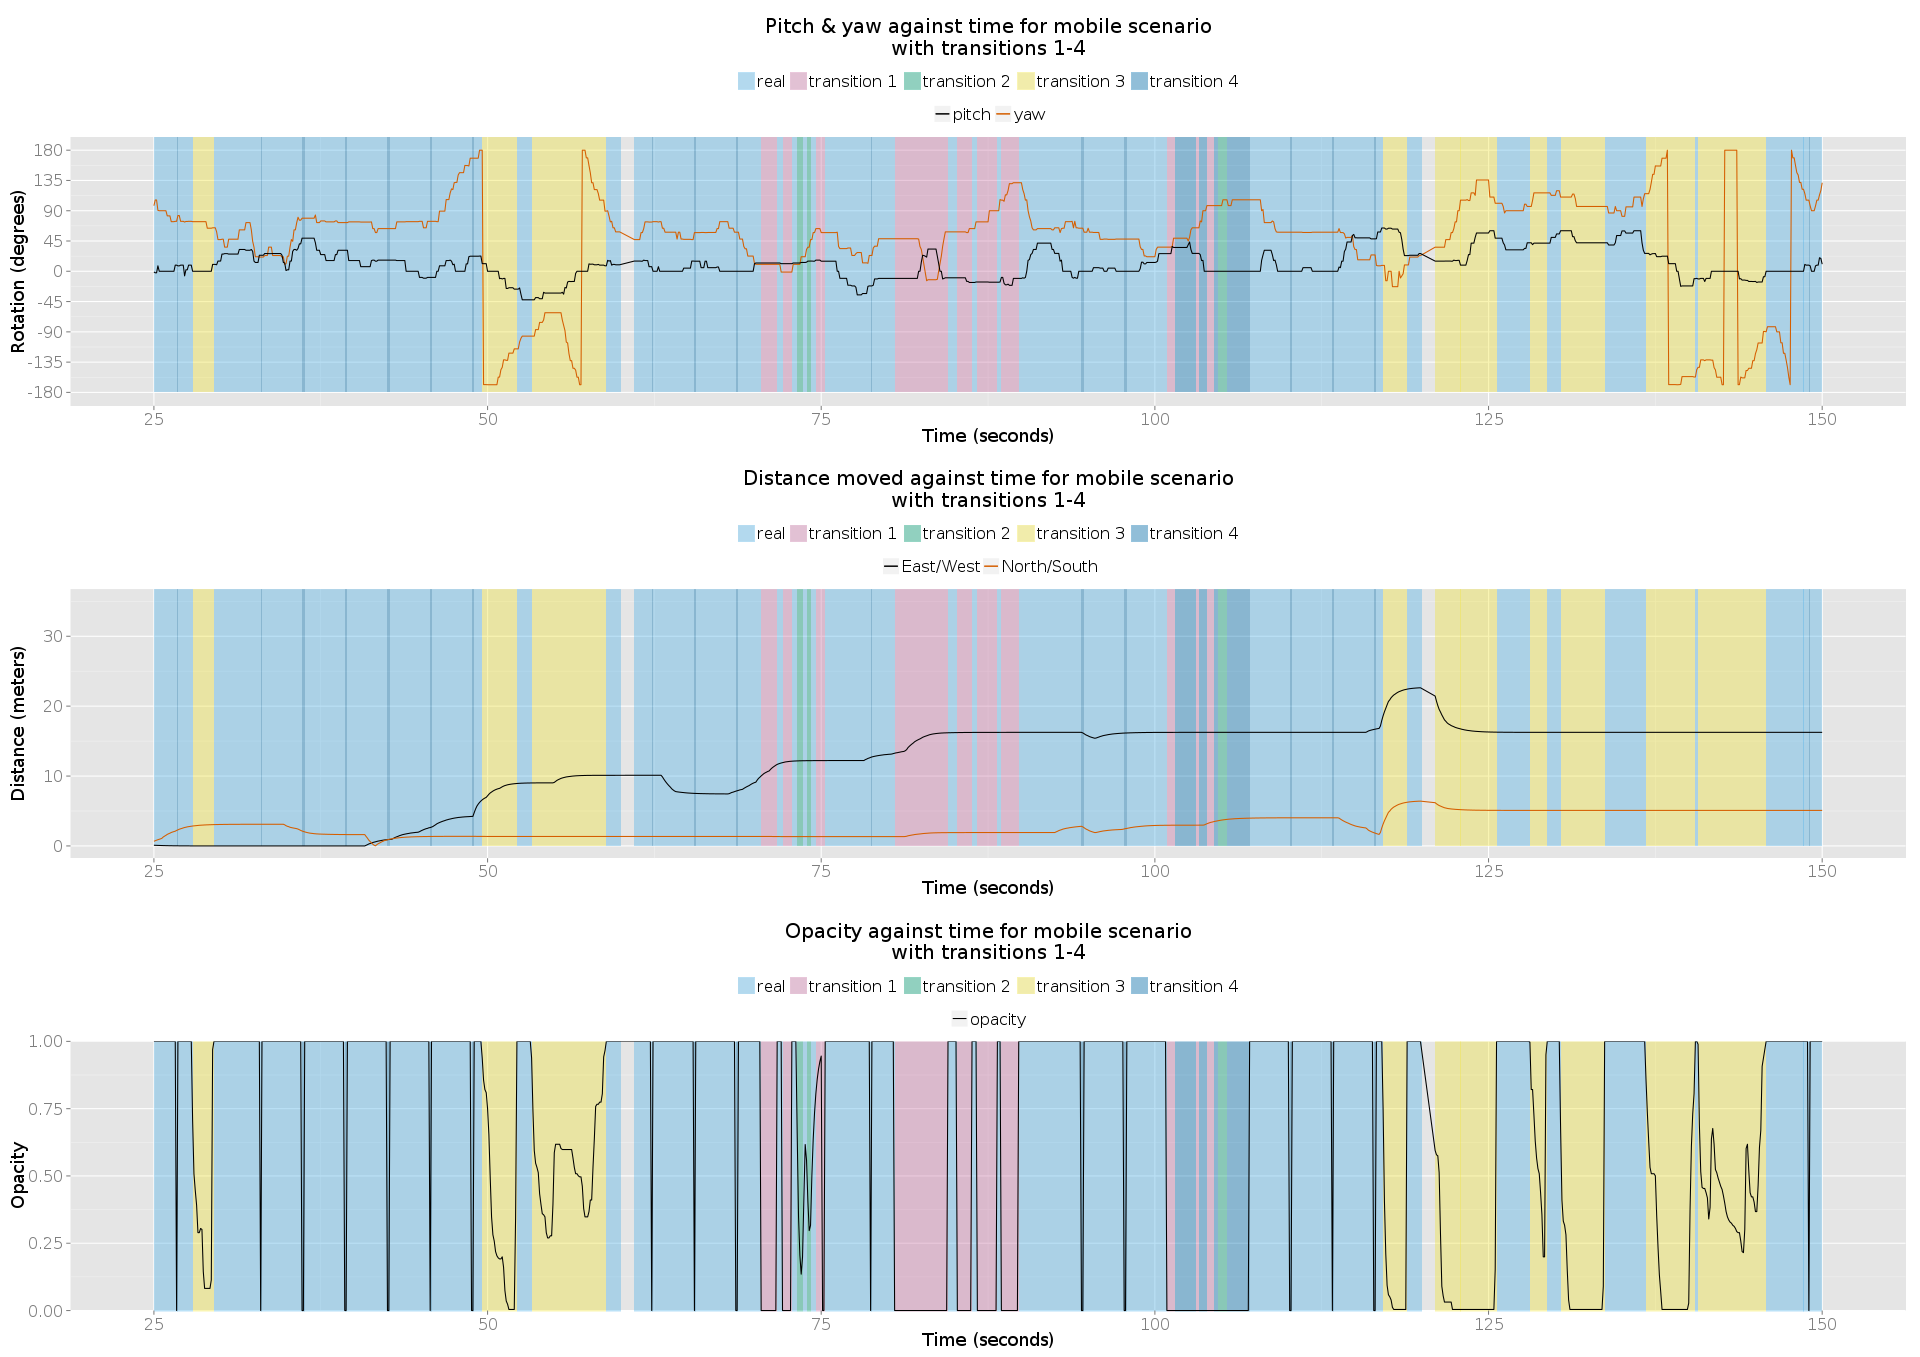
\includegraphics[width=\textwidth]{2.1/12_1-4_3up.png}
	\caption{Some images, yah.}
	\end{center}
\end{figure}

%=========================================================================================================

\clearpage

\subsection{Participant 13}

\begin{figure}[h]
	\begin{center}
	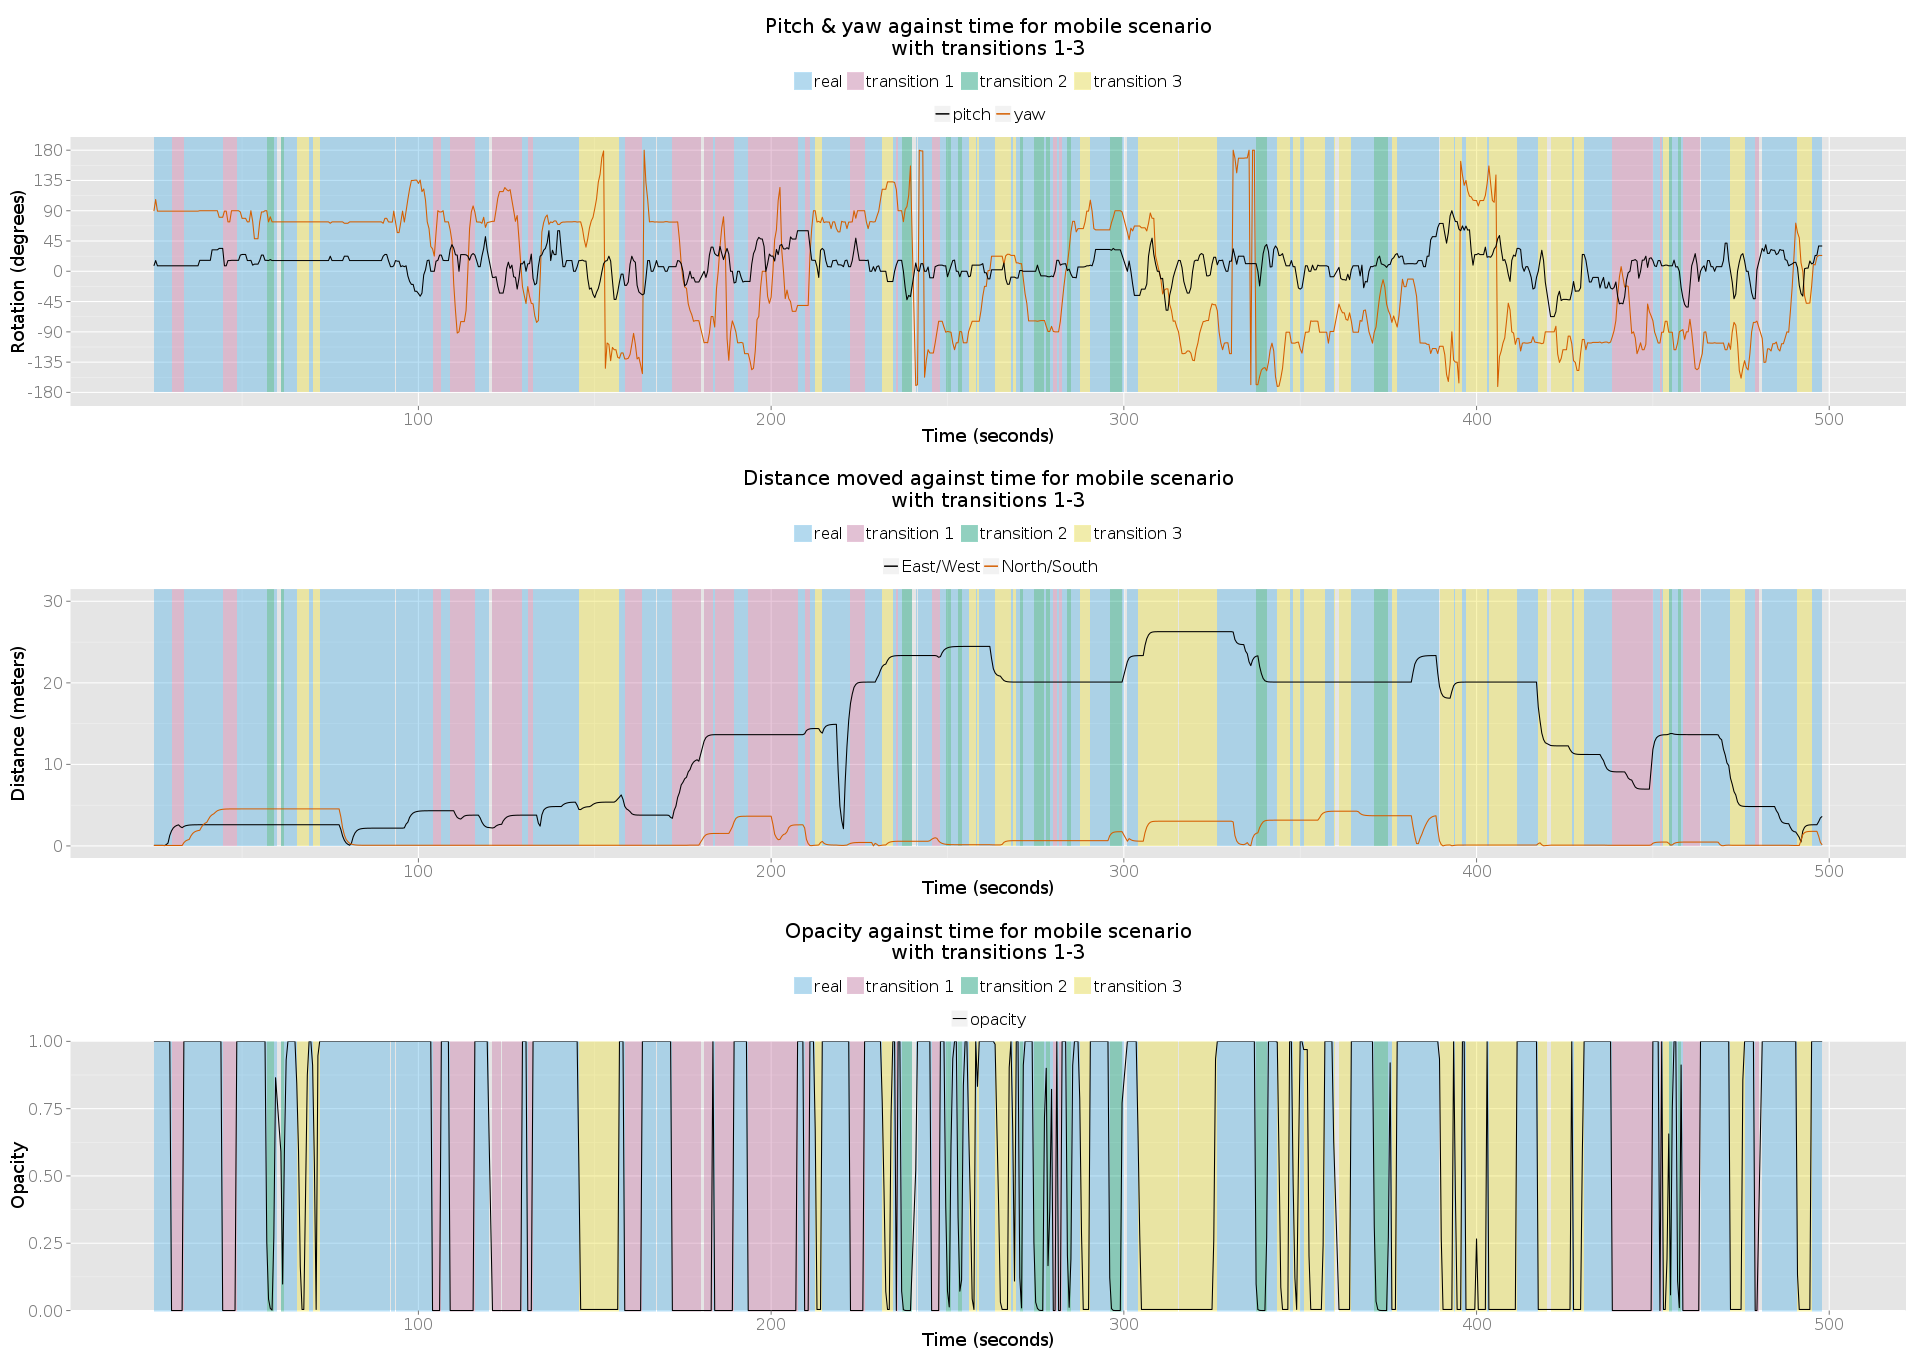
\includegraphics[width=\textwidth]{2.1/13_1-3_3up.png}
	\caption{Some images, yah.}
	\end{center}
\end{figure}

\clearpage

\begin{figure}[h]
	\begin{center}
	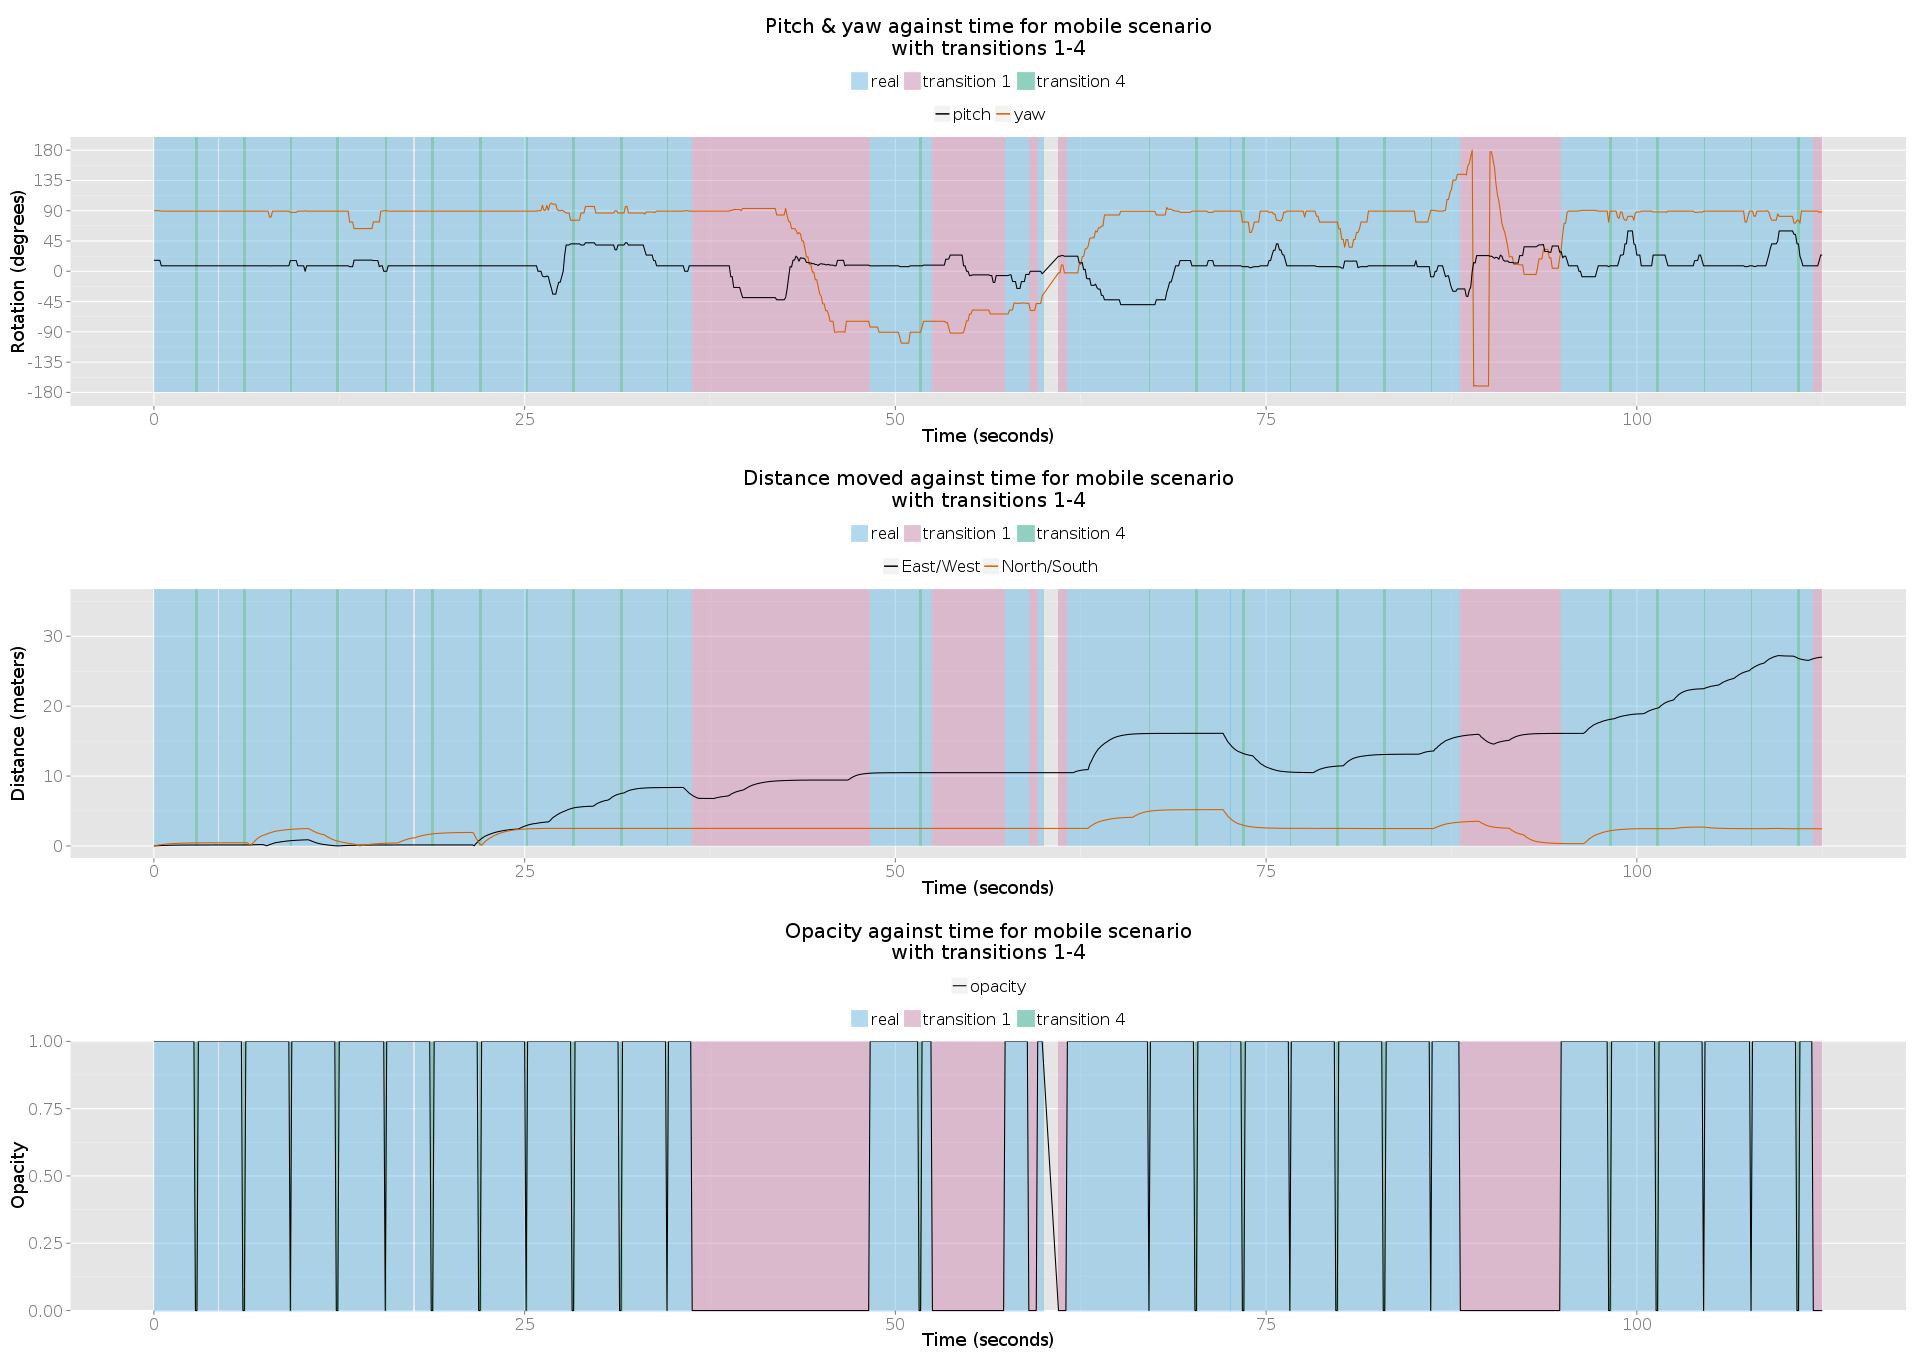
\includegraphics[width=\textwidth]{2.1/13_1-4_3up.png}
	\caption{Some images, yah.}
	\end{center}
\end{figure}

%=========================================================================================================

\clearpage

\section{Phase 2.2 Results}

%=========================================================================================================

\clearpage

\subsection{Participant 14}

\begin{figure}[h]
	\begin{center}
	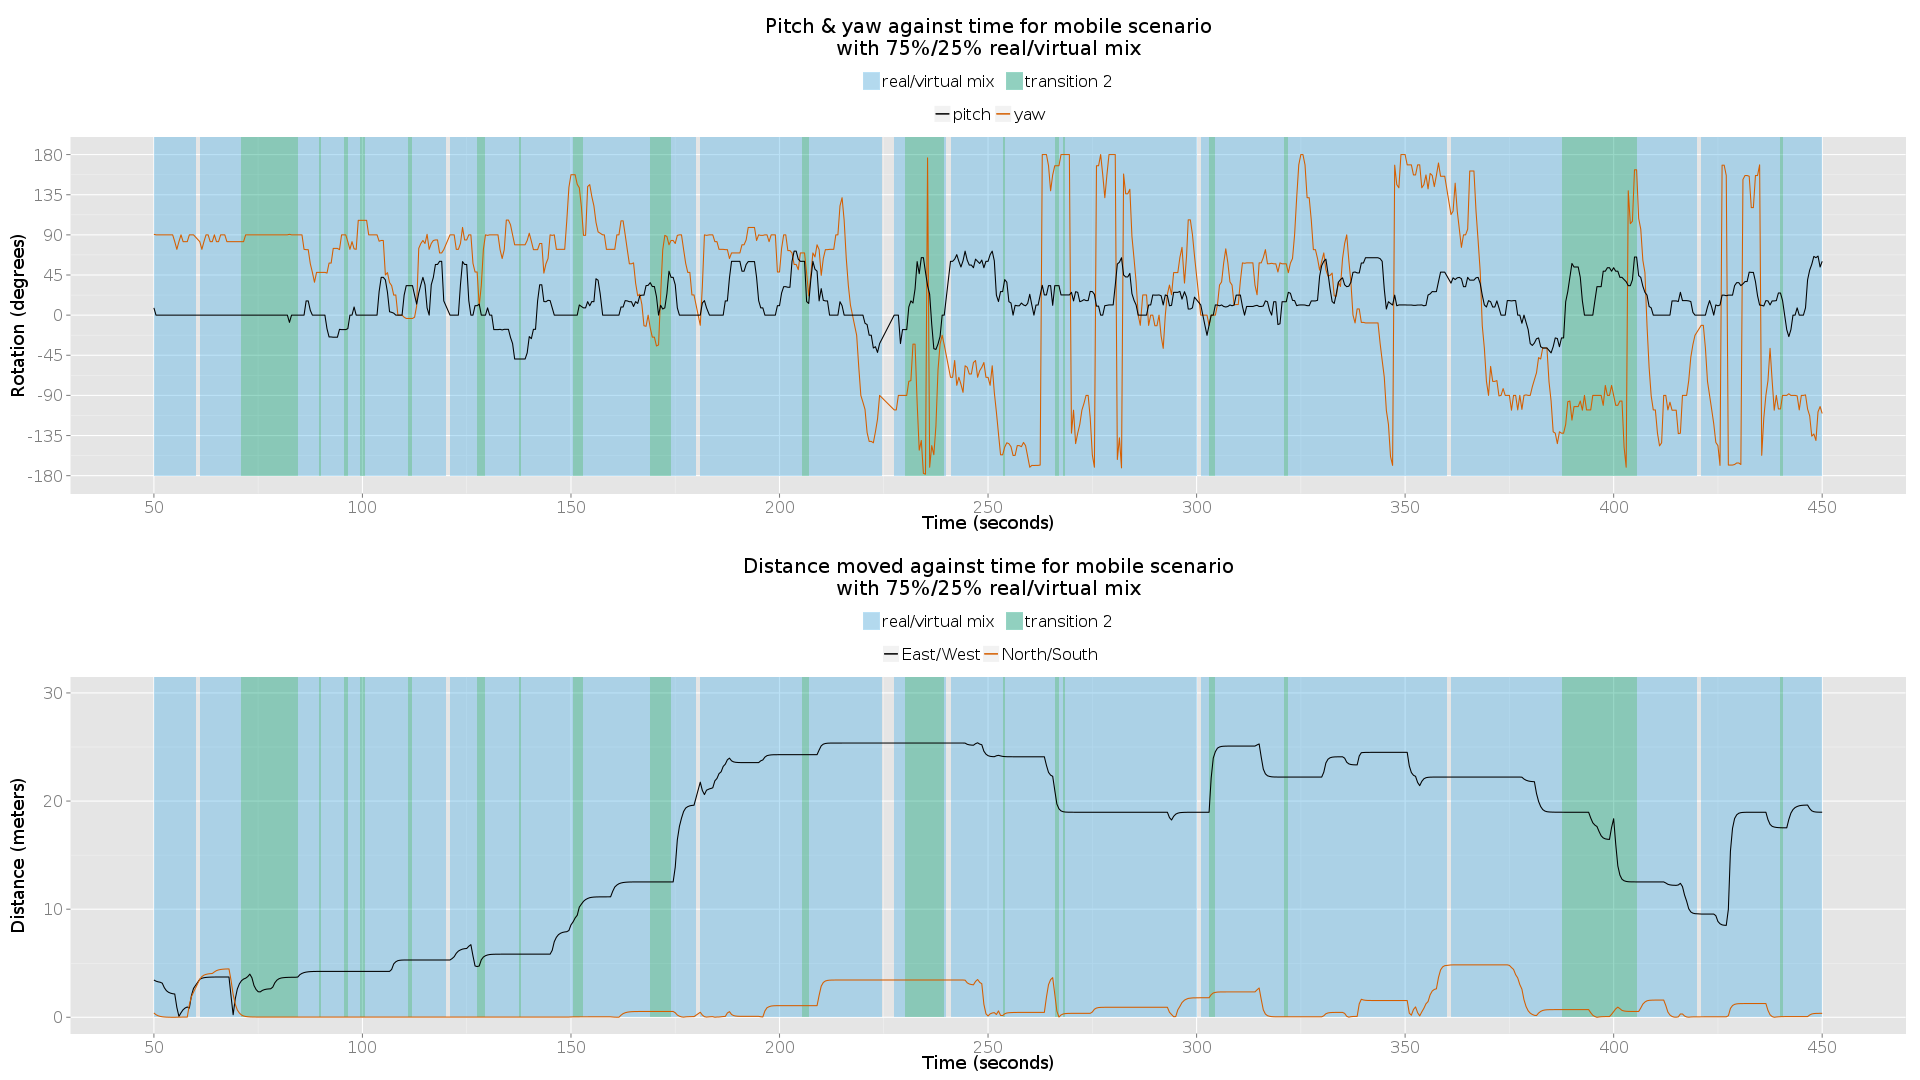
\includegraphics[width=\textwidth]{2.2/14_75_2up.png}
	\caption{Some images, yah.}
	\end{center}
\end{figure}

\clearpage

\begin{figure}[h]
	\begin{center}
	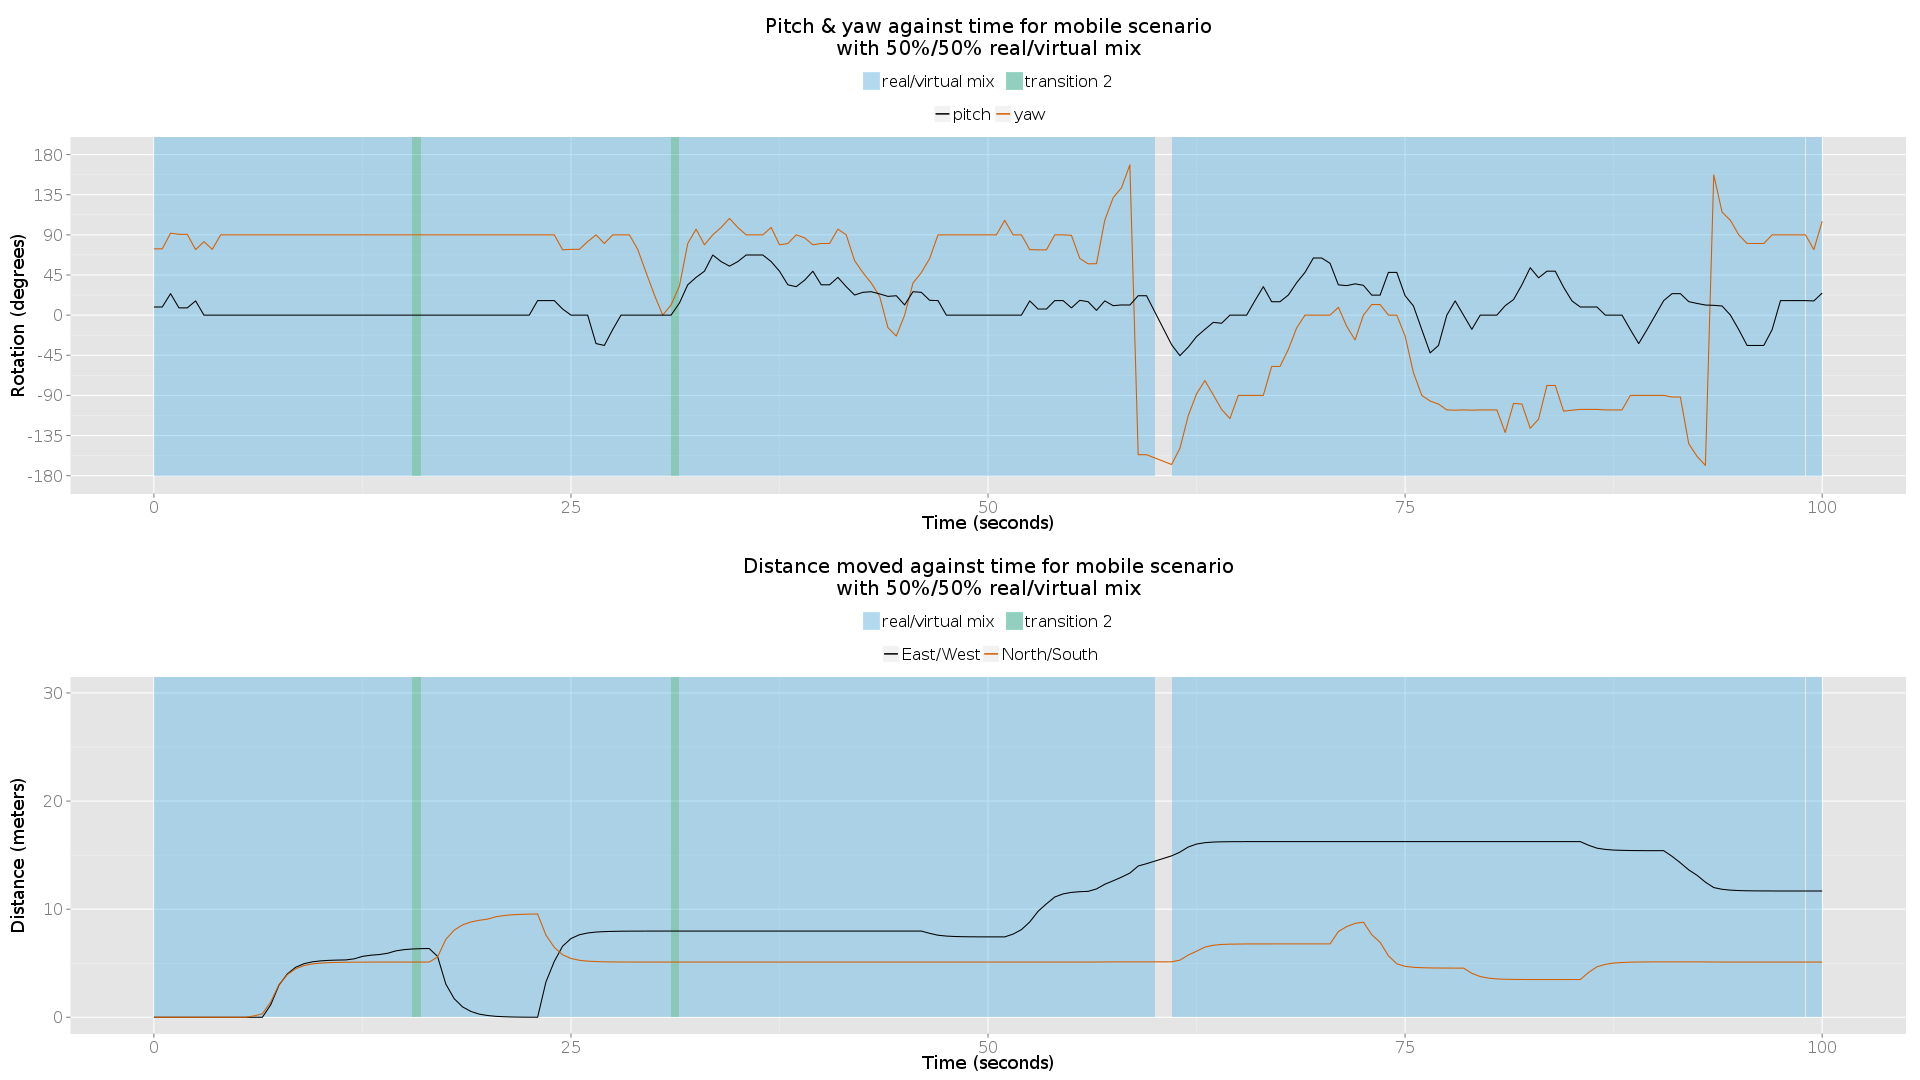
\includegraphics[width=\textwidth]{2.2/14_50_2up.png}
	\caption{Some images, yah.}
	\end{center}
\end{figure}

%=========================================================================================================

\clearpage

\subsection{Participant 15}

\begin{figure}[h]
	\begin{center}
	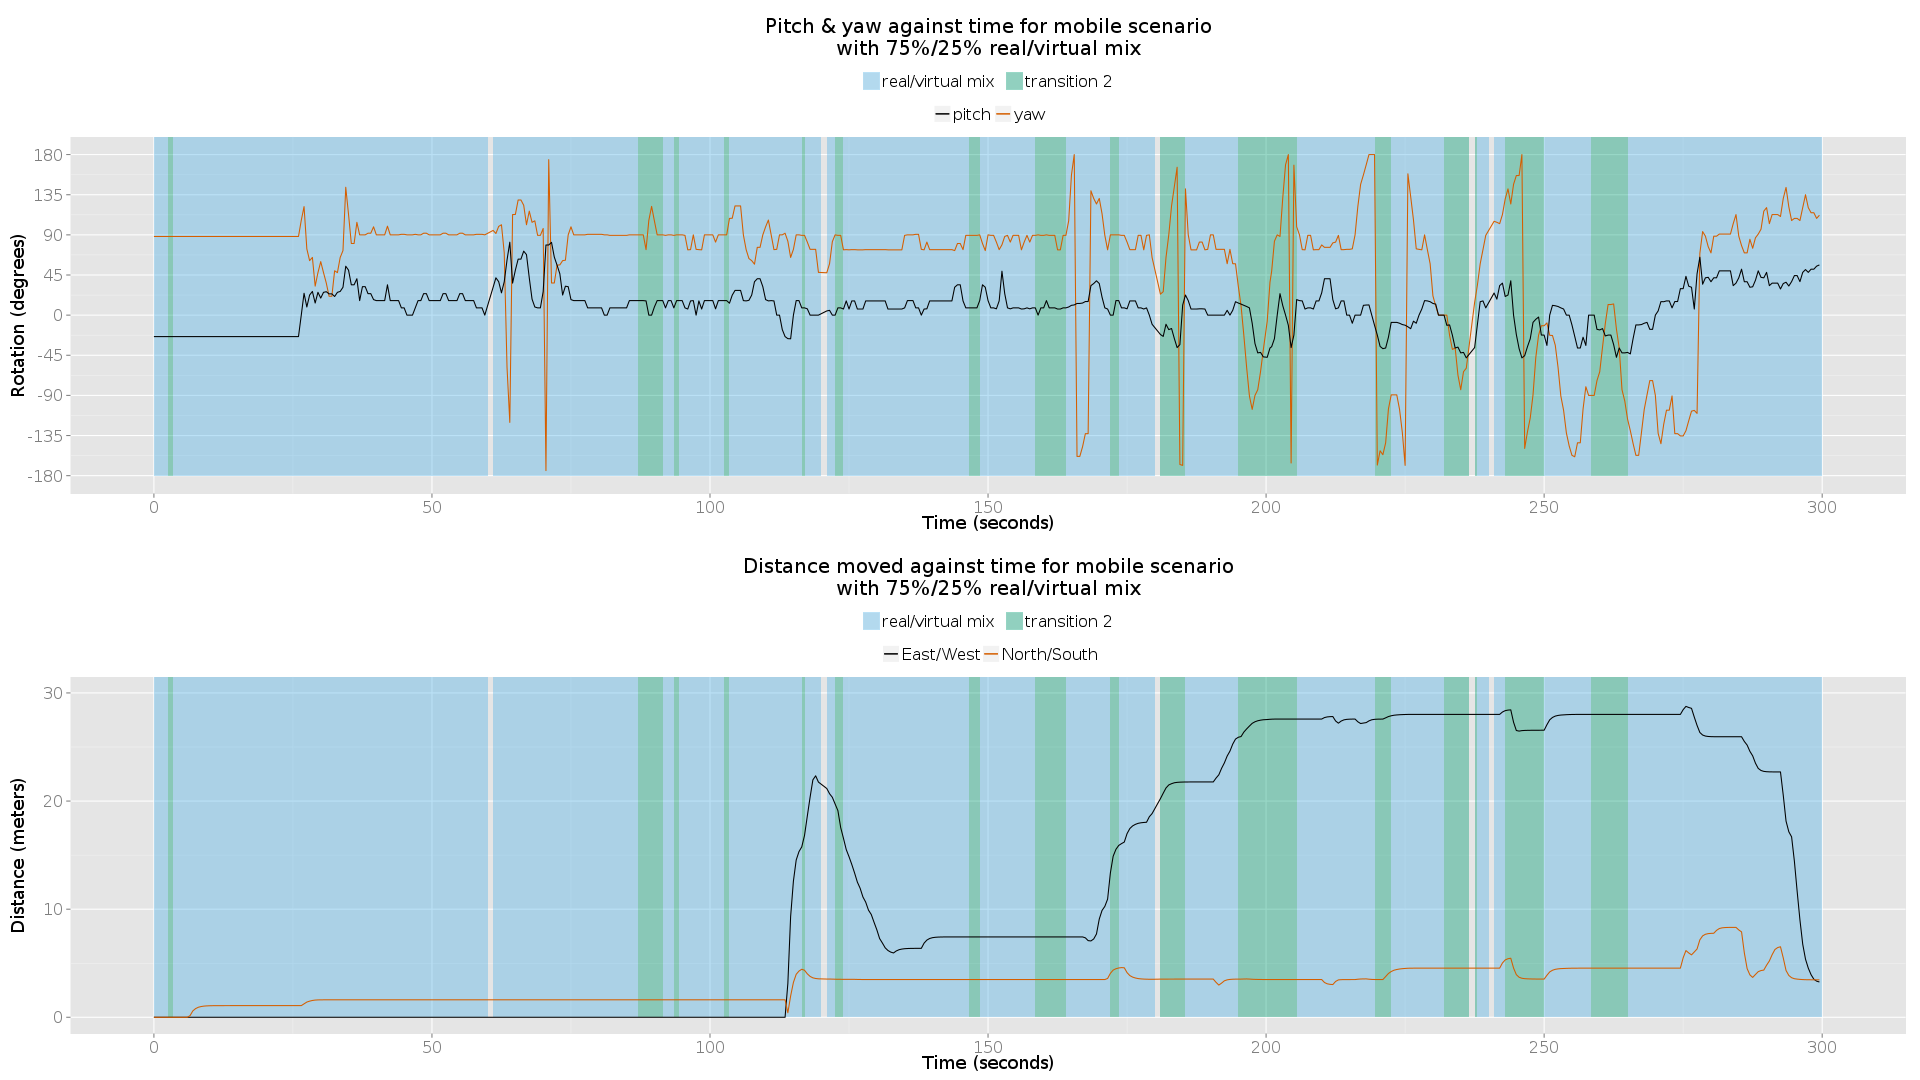
\includegraphics[width=\textwidth]{2.2/15_75_2up.png}
	\caption{Some images, yah.}
	\end{center}
\end{figure}

\clearpage

\begin{figure}[h]
	\begin{center}
	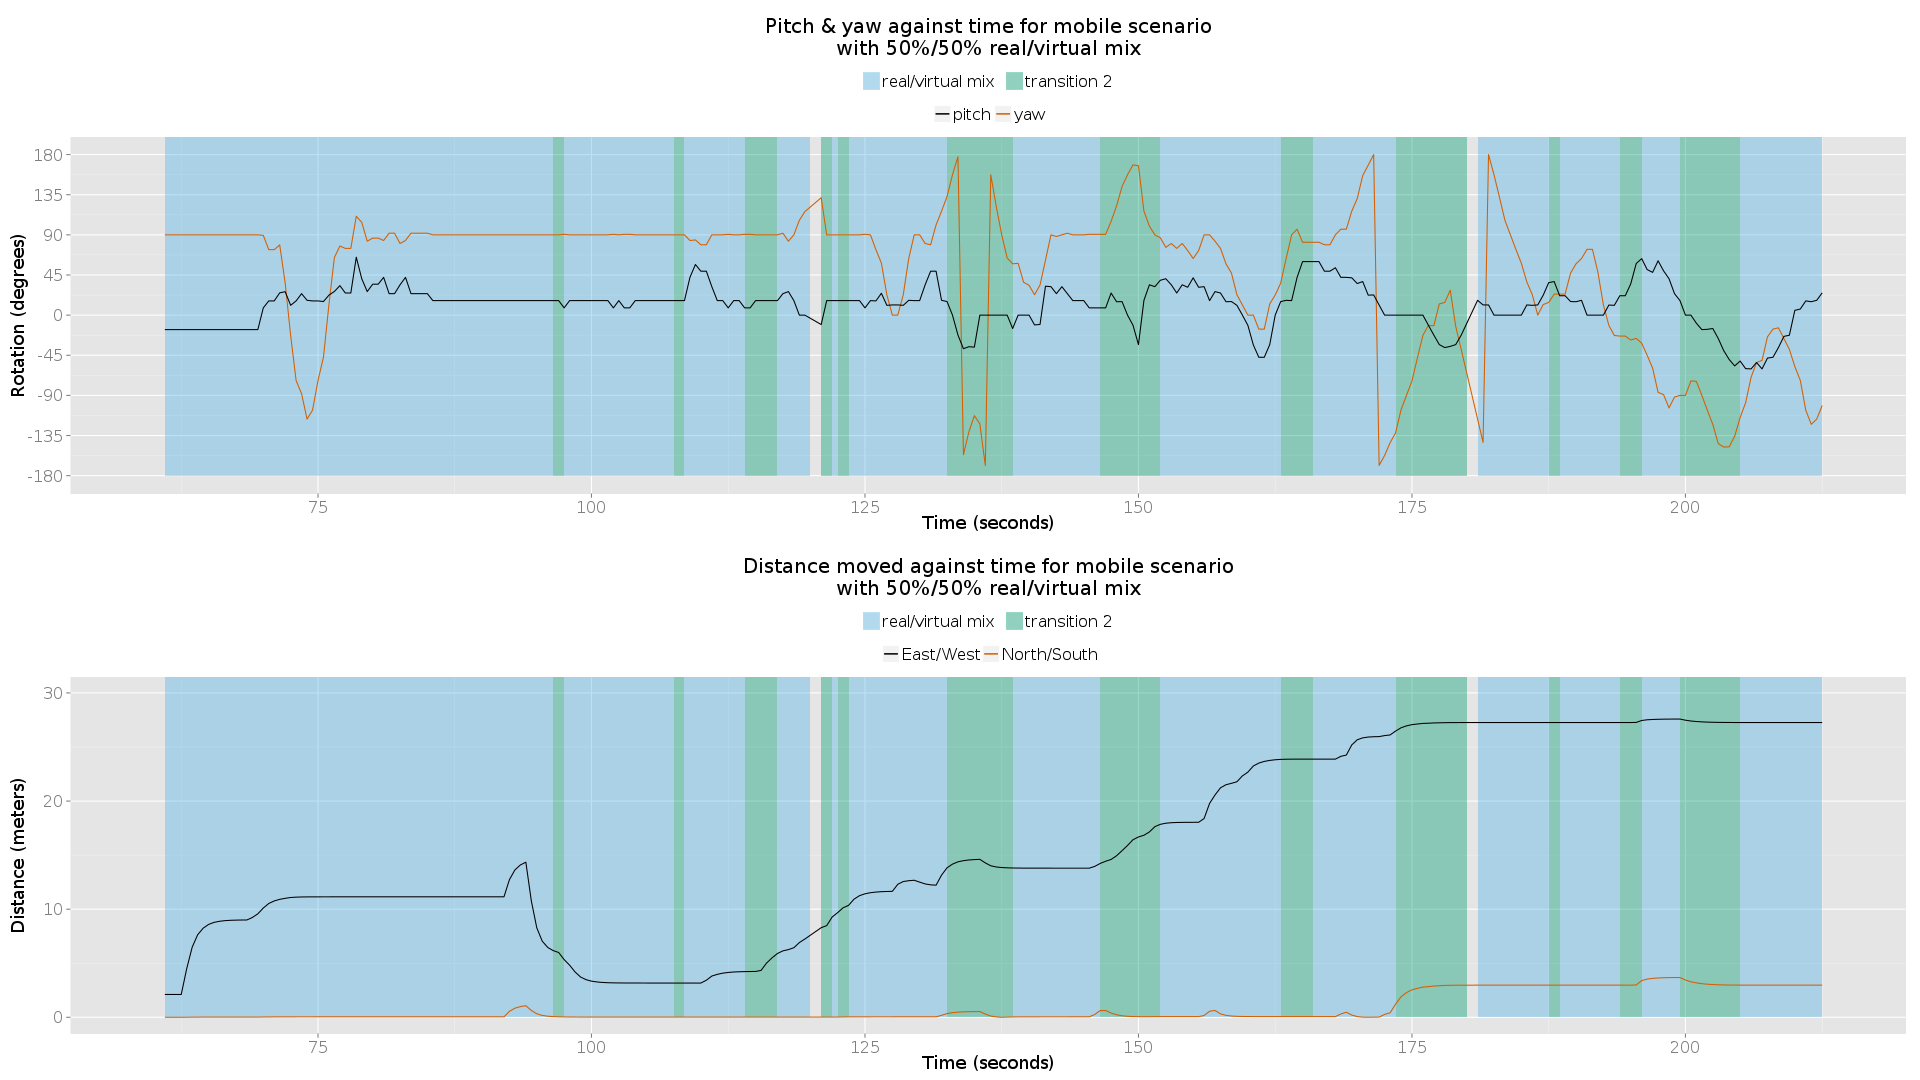
\includegraphics[width=\textwidth]{2.2/15_50_2up.png}
	\caption{Some images, yah.}
	\end{center}
\end{figure}

%=========================================================================================================

\clearpage

\subsection{Participant 16}

\begin{figure}[h]
	\begin{center}
	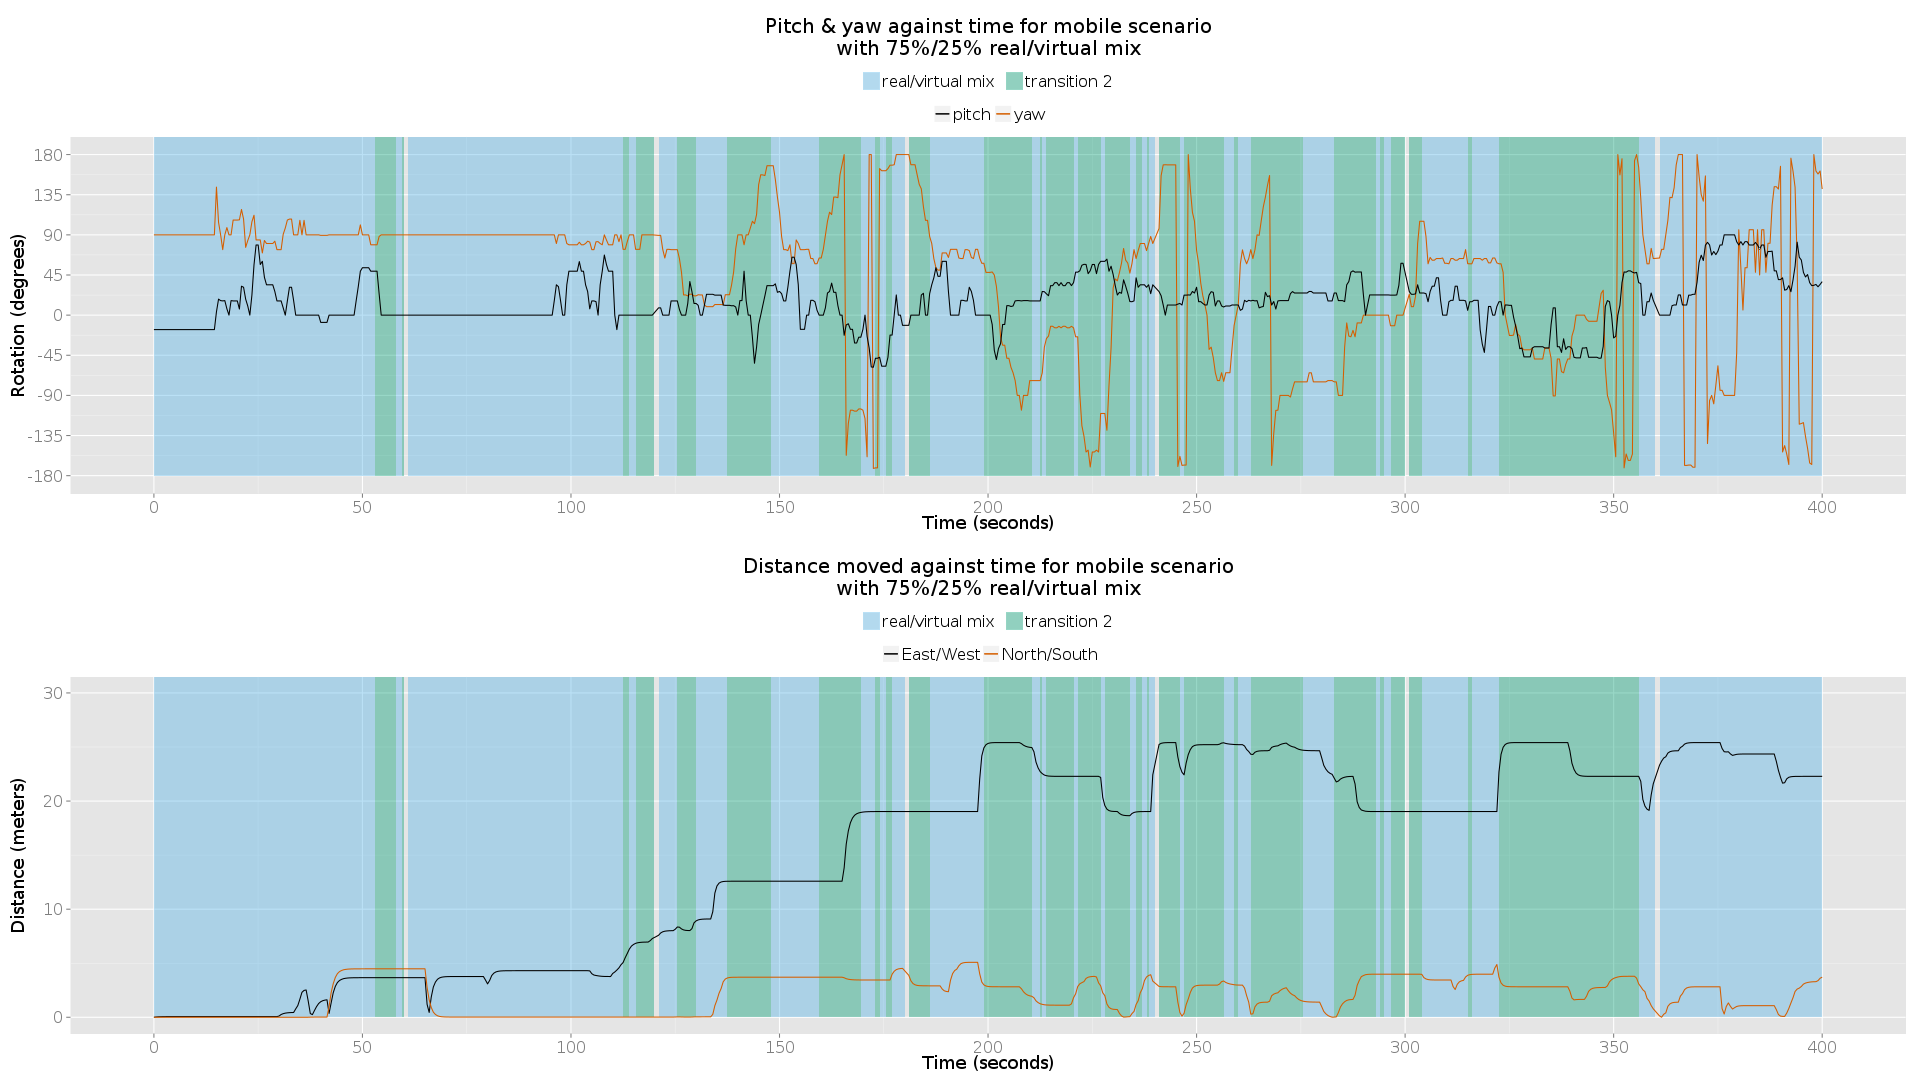
\includegraphics[width=\textwidth]{2.2/16_75_2up.png}
	\caption{Some images, yah.}
	\end{center}
\end{figure}

\clearpage

\begin{figure}[h]
	\begin{center}
	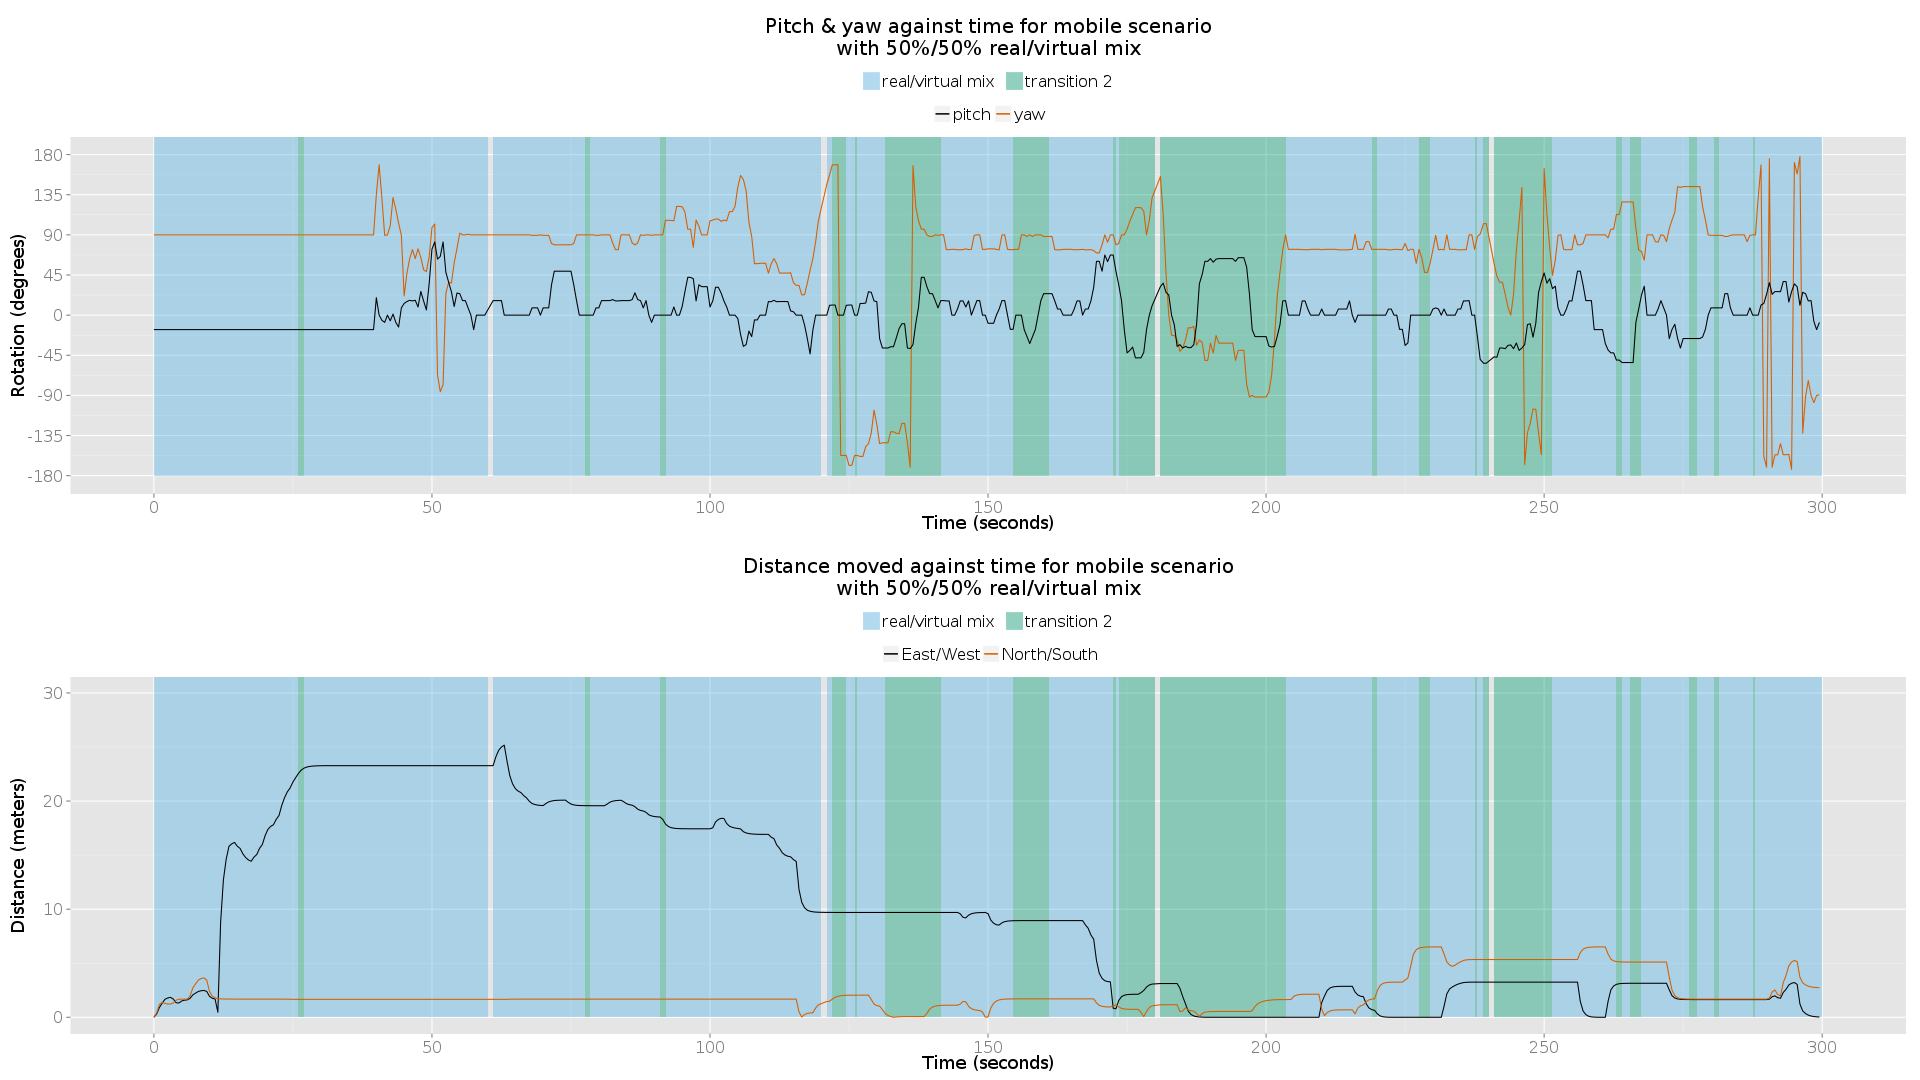
\includegraphics[width=\textwidth]{2.2/16_50_2up.png}
	\caption{Some images, yah.}
	\end{center}
\end{figure}

%=========================================================================================================

\clearpage

\subsection{Participant 17}

\begin{figure}[h]
	\begin{center}
	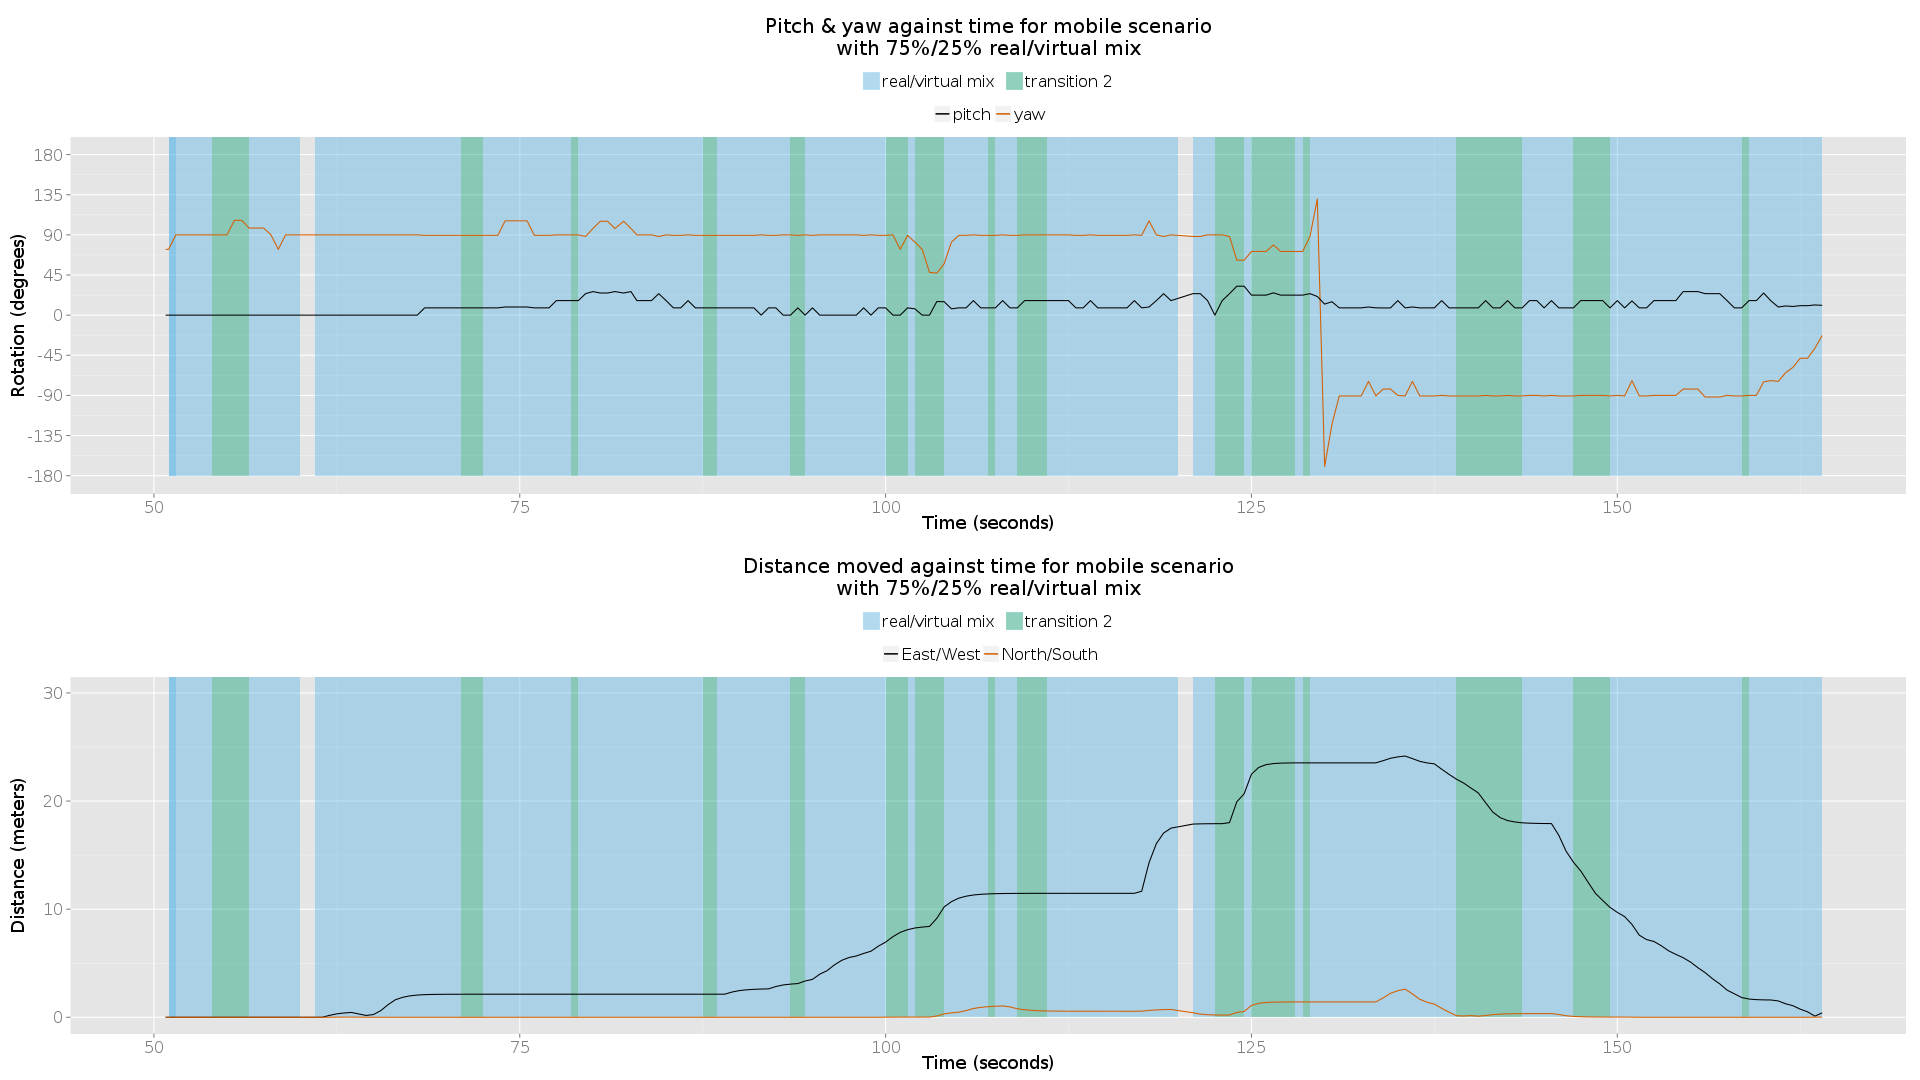
\includegraphics[width=\textwidth]{2.2/17_75_2up.png}
	\caption{Some images, yah.}
	\end{center}
\end{figure}

\clearpage

\begin{figure}[h]
	\begin{center}
	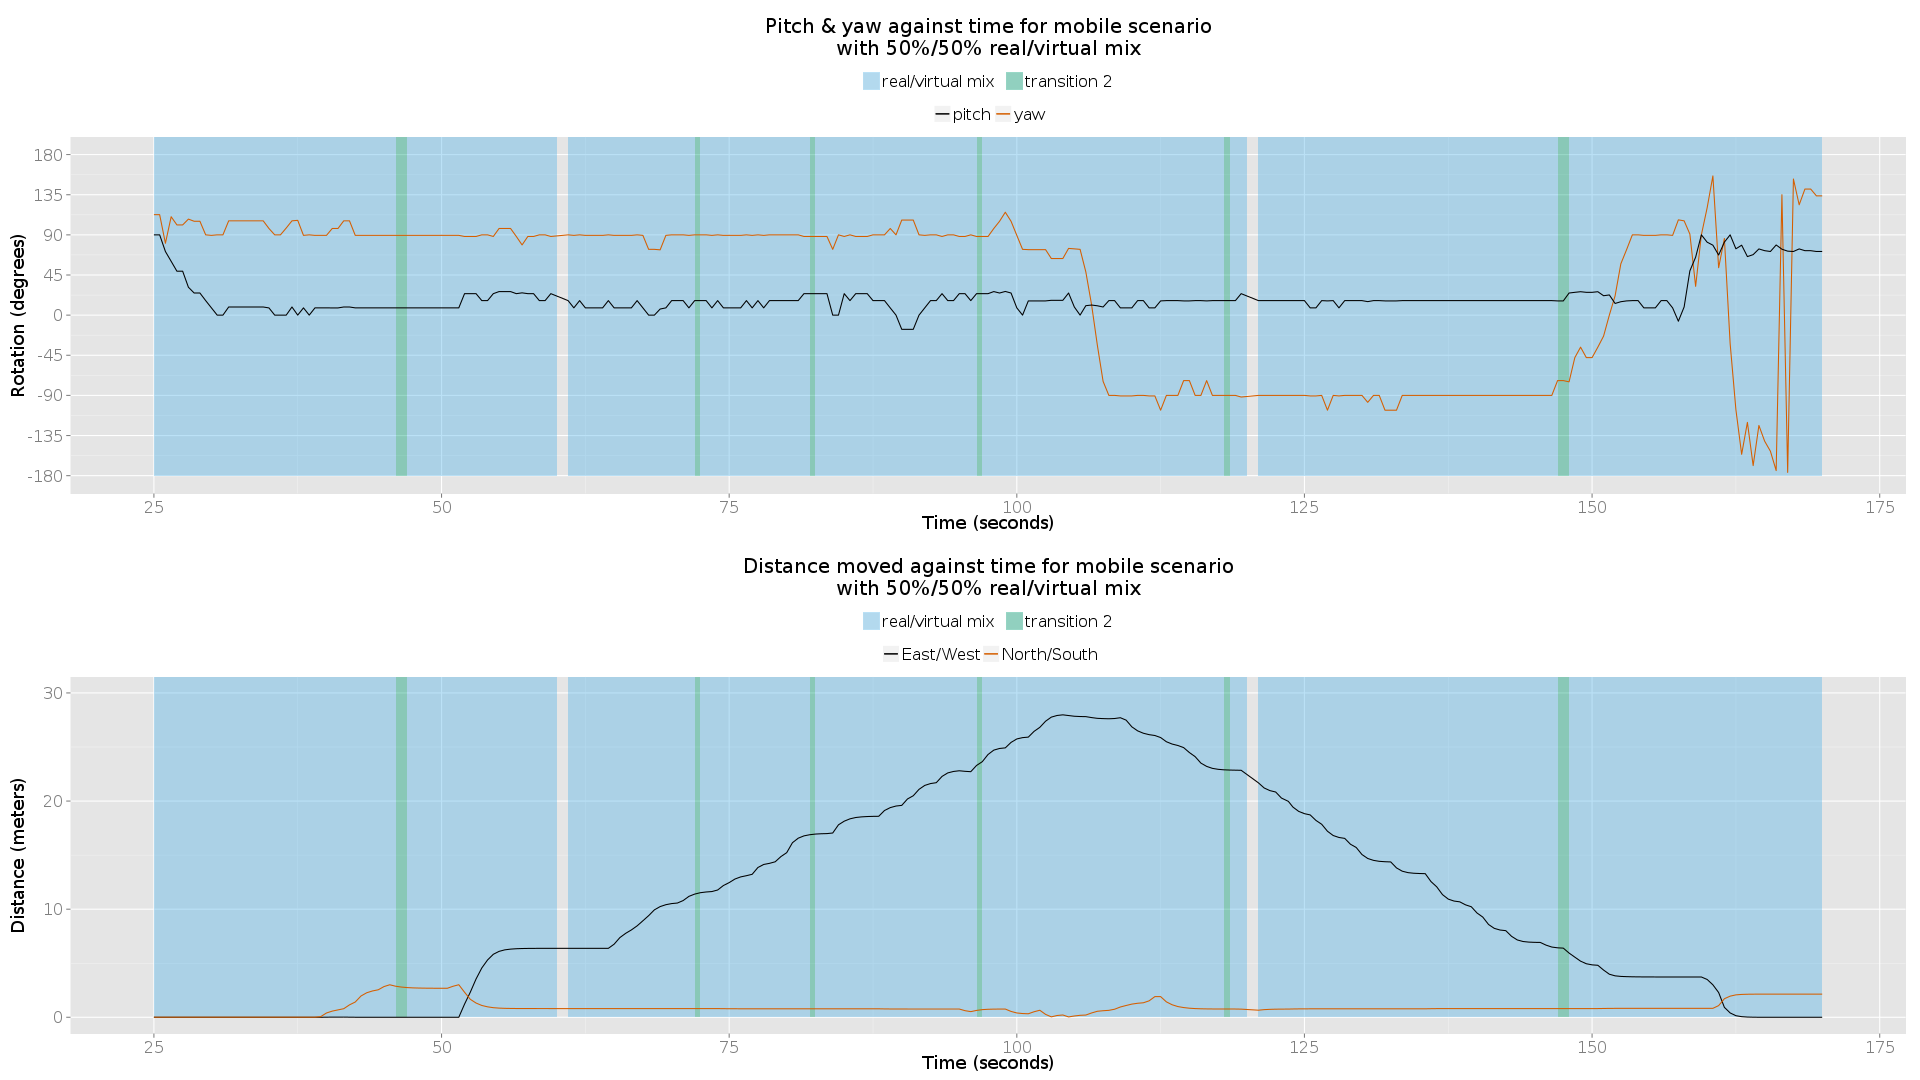
\includegraphics[width=\textwidth]{2.2/17_50_2up.png}
	\caption{Some images, yah.}
	\end{center}
\end{figure}

%=========================================================================================================